\documentclass[11pt]{article}

% ── Math (load BEFORE unicode-math per mathtools warning) ─────────────
\usepackage{mathtools}  % extends amsmath
\usepackage{amsthm}
\usepackage{xfrac}

% ── Fonts & encoding ─────────────────────────────────────────────────
\usepackage{fontspec}
\usepackage{unicode-math}
\setmainfont{Latin Modern Roman}
\setmathfont{Latin Modern Math}

% ── Layout ────────────────────────────────────────────────────────────
\usepackage[margin=1in]{geometry}
\usepackage{setspace}
\onehalfspacing
\setlength{\parskip}{3pt plus 1pt minus 1pt}

% ── Structure ─────────────────────────────────────────────────────────
\usepackage{enumitem}
\usepackage{booktabs}
\usepackage{array}
\usepackage{longtable}
\usepackage[most]{tcolorbox}
\tcbuselibrary{skins,breakable}

% ── B&W boxes ─────────────────────────────────────────────────────────
\newtcolorbox{axiombox}{
  colback=white, colframe=black,
  sharp corners, boxrule=0.8pt,
  left=8pt, right=8pt, top=6pt, bottom=6pt
}

\newtcolorbox{lemmabox}{
  colback=black!3, colframe=black,
  sharp corners, boxrule=0.8pt,
  left=8pt, right=8pt, top=6pt, bottom=6pt
}

\newtcolorbox{resultbox}[1][]{
  colback=black!3, colframe=black!60,
  fonttitle=\bfseries\sffamily\small, title={#1},
  sharp corners, boxrule=0.6pt,
  left=8pt, right=8pt, top=5pt, bottom=5pt
}

\newtcolorbox{tensionbox}[1][]{
  colback=black!3, colframe=black!60,
  fonttitle=\bfseries\sffamily\small, title={#1},
  sharp corners, boxrule=0.6pt,
  left=8pt, right=8pt, top=5pt, bottom=5pt
}

\newtcolorbox{layerbox}[2][]{
  colback=black!3, colframe=black!60,
  fonttitle=\bfseries\sffamily\small, title={#1},
  sharp corners, boxrule=0.6pt,
  left=8pt, right=8pt, top=5pt, bottom=5pt
}

% ── apfbox style (used in body) ───────────────────────────────────────
\tcbset{
    apfbox/.style={
        enhanced,
        colback=black!3,
        frame hidden,
        borderline={0.5pt}{0pt}{black},
        arc=0pt,
        left=8pt, right=8pt, top=8pt, bottom=8pt,
        fonttitle=\bfseries\color{black},
        coltitle=black,
        detach title,
        before upper={\tcbtitle.\enspace},
        before skip=14pt,
        after skip=14pt,
        grow to left by=-8pt,
        grow to right by=-8pt,
        sharp corners,
        breakable,
    }
}

% ── Section formatting ────────────────────────────────────────────────
\usepackage{tikz}
\usetikzlibrary{shapes,arrows.meta,positioning}
\usepackage{titlesec}
\titleformat{\section}{\Large\bfseries}{\thesection.}{0.5em}{}
\titleformat{\subsection}{\large\bfseries}{\thesubsection}{0.5em}{}
\titleformat{\subsubsection}{\normalsize\bfseries}{\thesubsubsection}{0.5em}{}

% ── Headers ───────────────────────────────────────────────────────────
\usepackage{fancyhdr}
\pagestyle{fancy}
\fancyhf{}
\fancyhead[L]{\small\itshape Paper 13: The Minimal Admissibility Core \textnormal{v8.1}}
\fancyhead[R]{\small\itshape E.\,Brooke}
\fancyfoot[C]{\thepage}
\renewcommand{\headrulewidth}{0.4pt}

% ── Hyperlinks (all black) ───────────────────────────────────────────
\usepackage[colorlinks=true,linkcolor=black,citecolor=black,urlcolor=black]{hyperref}

% ── Shorthand ─────────────────────────────────────────────────────────
\providecommand{\square}{\ensuremath{\mdlgwhtsquare}}
\newcommand{\A}{\mathrm{A1}}
\newtheorem{proposition}{Proposition}[section]
\newcommand{\Ctot}{C_{\mathrm{total}}}
\newcommand{\deff}{d_{\mathrm{eff}}}
\newcommand{\Adm}{\mathrm{Adm}}
\newcommand{\OmL}{\Omega_\Lambda}
\newcommand{\Omm}{\Omega_m}
\newcommand{\Omb}{\Omega_b}
\newcommand{\OmDM}{\Omega_{\mathrm{DM}}}
\newcommand{\sw}{\sin^2\!\theta_W}
\newcommand{\fb}{f_b}
\newcommand{\Ngen}{N_{\mathrm{gen}}}
\newcommand{\LG}{\Lambda \cdot G}
\newcommand{\eps}{\varepsilon}
\newcommand{\Lnc}{L_{\mathrm{nc}}}
\newcommand{\Lloc}{L_{\mathrm{loc}}}
\newcommand{\Lirr}{L_{\mathrm{irr}}}
\newcommand{\Lcol}{L_{\mathrm{col}}}
\newcommand{\Leps}{L_{\eps^*}}
% ── Extra macros from V2 body ─────────────────────────────────────────
\newcommand{\Aut}{\mathrm{Aut}}
\newcommand{\tr}{\mathrm{tr}}
\newcommand{\SU}{\mathrm{SU}}
\newcommand{\U}{\mathrm{U}}
\newcommand{\nats}{\;\mathrm{nats}}
\DeclareMathOperator*{\argmin}{arg\,min}

\begin{document}

% ── Title ─────────────────────────────────────────────────────────────
\thispagestyle{empty}
\begin{center}
  {\LARGE\bfseries Paper 13: The Minimal Admissibility Core}\\[6pt]
  {\Large Version 8.1}\\[14pt]
  {\large E.\,S.\,Brooke}\\[4pt]
  {\normalsize February 2026}\\[16pt]
  {\small\sffamily APF codebase \quad$\cdot$\quad 129 theorems \quad$\cdot$\quad 8 modules \quad$\cdot$\quad 827 assertions \quad$\cdot$\quad 0 free parameters}
\end{center}

\vspace{10pt}

\begin{abstract}
\noindent
Nature cannot maintain an infinite number of distinctions simultaneously.  This single constraint---that the universe's capacity to enforce observable differences is finite---turns out to be extraordinarily powerful.  We show that from this axiom alone (which we call A1: finite enforcement capacity), the entire architecture of modern physics is logically forced: Hilbert space and quantum mechanics, the gauge symmetries of the Standard Model, four-dimensional spacetime, Einstein's equations, and the specific numerical values of constants that standard physics treats as unexplained inputs.  The framework does not model physics---it derives it, from one axiom and zero free parameters.

This paper presents the complete derivation in self-contained form.  Detailed proofs are developed across the companion papers: Paper~1 (\textit{SPINE}) through Paper~7 (\textit{ACTION}) and \textit{Gauge Theory from Finite Distinguishability}, each treating one layer of the derivation chain; cross-references are given throughout, with key derivations included in this paper's appendices.

The framework makes contact with reality at three distinct layers: (I)~structural necessities forced by the axiom (Hilbert space, gauge symmetry, $d{=}4$ spacetime); (II)~exact rational predictions from capacity counting ($\sin^2\!\theta_W = 3/13$, $\Omega_\Lambda = 42/61$, $f_b = 3/19$, $\Lambda\cdot G = 3\pi/102^{61}$); and (III)~model-dependent estimates using framework-derived inputs ($n_s$, $\eta_B$, BBN abundances).  We present the full observational concordance---12 predictions, 0 free parameters---with honest epistemic stratification and explicit identification of tensions and attack surfaces.

The derivation chain is: one axiom produces four lemmas (locality, non-closure, irreversibility, minimality), which produce 129 machine-verifiable theorems across 8 physics modules, which produce 25 quantitative predictions (including cosmological densities, the Weinberg angle, all three PMNS neutrino mixing angles, all CKM quark mixing parameters, and six fermion mass ratios), 6 qualitative predictions, and 11 principles normally assumed as axioms---all from zero free parameters (Appendix~F).  The APF codebase (827 assertions, all passing, zero empirical imports in the derivation chain) serves as the authoritative specification: every claim in this paper can be checked against running code.
\end{abstract}

\tableofcontents
\newpage

% ══════════════════════════════════════════════════════════════════
% PART I: FOUNDATIONS
% ══════════════════════════════════════════════════════════════════

{\centering\Large\bfseries Part I: Foundations\par}
\addcontentsline{toc}{part}{Part I: Foundations}
\vspace{8pt}

% ── Section 1 ────────────────────────────────────────────────────
\section{Introduction}

\subsection{The Central Claim}

Physical theories are conventionally presented as dynamical frameworks: they specify a space of states and laws governing their evolution.  Those laws are written based on what we observe---particles, forces, fields---and describe their interactions.  But the particles and forces themselves are inputs to the theory, not outputs.  The Standard Model does not explain why there are three generations of fermions, or why the gauge group is $\SU(3)\times\SU(2)\times\U(1)$.  It assumes them.

This paper starts from a different place.  Rather than assuming what exists and writing laws to describe it, we treat the universe as a finite system and ask what that finiteness alone requires.  The answer is surprisingly specific: finiteness does not merely constrain the theory---it determines it.

The key insight is that distinctions are not free.  A physical distinction---between two states, two outcomes, two histories---is meaningful only if something actively prevents it from washing out.  If two alternatives can merge back together at no cost, the distinction between them was never physical.  Maintaining a distinction requires enforcement, and enforcement costs resources.  If those resources were unlimited, every conceivable distinction would be real---there would be no structure, no selection, no physics.  That is not the universe we observe.  Ours has specific particles, specific forces, specific constants---which means enforcement is finite, and the budget is what determines the inventory.

This leads to a single axiom: the total enforcement capacity is finite.  From this axiom alone---with no choice of particles, gauge groups, or spacetime dimension---the Standard Model emerges as the unique theory compatible with finite enforceability.

\subsection{Roadmap}

Part~I (Sections 1--7) establishes the mathematical structure: the axiom, its formal consequences, the derivation chain from axiom to derived lemmas, the canonical mathematical object, and its computational applications.  Part~II (Sections 8--12) maps that structure onto physical reality, presenting the three-layer epistemic architecture, the complete derivation chain from axiom to observables, the full concordance scorecard, and an honest accounting of tensions and attack surfaces.

% ── EDIT 3: APF engine discussion and file references ────────────
\medskip
\noindent\textit{The APF codebase as specification.}\quad Throughout this paper we reference specific verification functions by name---for example, \texttt{check\_T22} in \texttt{generations.py}.  These refer to the Admissibility Physics Framework (APF) codebase, which serves as the executable specification of every theorem presented here.  The APF is organized as a modular Python package with eight physics modules, each corresponding to a layer of the derivation chain (see Appendix~E for the full module table and theorem index).  When this paper states ``(check\_T22, generations.py)'', it means: the claim can be verified by running the corresponding function.  The code is the authoritative specification; the prose is a guide to reading it.

\medskip
\noindent\textit{Companion papers.}\quad This paper is self-contained but draws on detailed derivations developed in the companion series.  The key references are:

\smallskip
\begin{itemize}[nosep,leftmargin=2em]
\item \textbf{Paper~1} --- SPINE: The Enforceability of Distinction---the foundational axiom, four lemmas, and the complete structural backbone~\cite{P1}.
\item \textbf{Paper~2} --- STRUCTURE: Non-Closure Under Composition---the formal development of $L_{\mathrm{nc}}$ and its constructive witnesses~\cite{P2}.
\item \textbf{Paper~3} --- LEDGERS: Entropy, Time, and Accumulated Cost as Capacity Accounting~\cite{P3}.
\item \textbf{Paper~4} --- CONSTRAINTS: Admissibility Constraints and Structural Saturation---monogamy, horizons, area laws, and the first derivations of $N_{\mathrm{gen}}=3$ and $\sin^2\!\theta_W = 3/13$~\cite{P4}.
\item \textbf{Paper~5} --- QUANTUM: Structure from Finite Enforceability---Hilbert space, Born rule, and CPTP maps from non-closure~\cite{P5}.
\item \textbf{Paper~6} --- DYNAMICS \& GEOMETRY as Optimal Admissible Reallocation---Einstein equations, $d=4$ spacetime, Lorentzian signature from smooth enforcement redistribution~\cite{P6}.
\item \textbf{Paper~7} --- A Minimal Quantum of ACTION from Finite Admissibility---structural necessity of quantization~\cite{P7}.
\item \textbf{Gauge Theory} --- Gauge Theory from Finite Distinguishability: A Reconstruction of the Standard Model from a Single Constraint---the Standard Model gauge group, complete field content, and cost closure~\cite{PGT}.
\end{itemize}
\smallskip

\noindent Where a derivation in this paper is presented in sketch form, the corresponding companion paper contains the full proof.  Cross-references are given throughout.


% ── Section 2 ────────────────────────────────────────────────────
\section{The Axiom: Finite Enforcement Capacity}

\subsection{What it says: every distinction costs something}

Consider any region of the universe.  Within that region, certain distinctions are being maintained: this particle is here, not there; this field has this value, not that one; this outcome occurred, not the alternative.  Each such distinction requires the universe to actively enforce it---to commit resources that prevent the distinction from washing out.

The axiom says: those resources are finite.  If each distinction~$d$ carries an enforcement cost $\varepsilon(d) > 0$, then the total cost of all distinctions maintained simultaneously cannot exceed some finite bound:
\begin{equation}
\sum_d \varepsilon(d) \;\le\; C < \infty
\end{equation}
We call $C$ the enforcement capacity of the region.

That is the entire physical input.  We do not specify what the distinctions are, how the enforcement works, or how much capacity is available.  The specific value of $C$ never matters; only finiteness and positivity enter any derivation.

\begin{figure}[ht]
\centering
\begin{tcolorbox}[
  enhanced, colback=white, colframe=black,
  boxrule=0.5pt, arc=0pt,
  left=6pt, right=6pt, top=6pt, bottom=6pt,
  sharp corners,
]
\centering
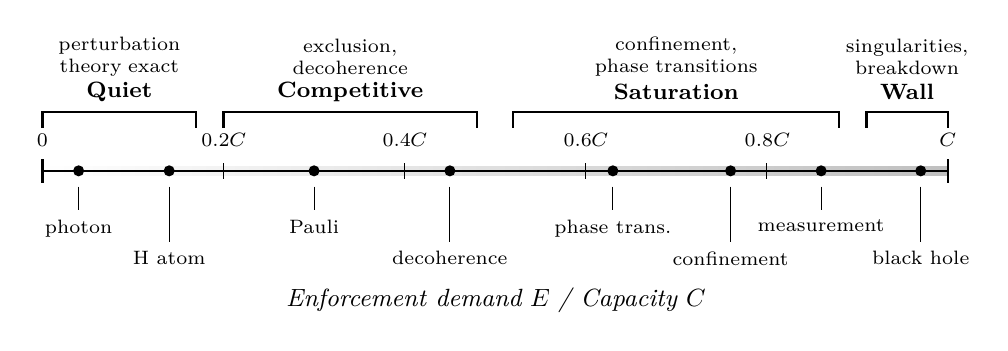
\begin{tikzpicture}[x=11.5cm, y=1cm]

% Gradient shading
\shade[left color=white, right color=black!25] (0,-0.06) rectangle (1,0.06);

% Main axis
\draw[thick] (0,0) -- (1,0);
\draw[thick] (0,-0.15) -- (0,0.15);
\draw[thick] (1,-0.15) -- (1,0.15);

% Tick marks and labels above axis
\foreach \x/\lab in {0/{0}, 0.2/{0.2$C$}, 0.4/{0.4$C$}, 0.6/{0.6$C$}, 0.8/{0.8$C$}, 1.0/{$C$}} {
  \draw (\x,-0.1) -- (\x,0.1);
  \node[above, font=\scriptsize] at (\x,0.18) {\lab};
}

% Regime brackets
\draw[thick] (0,0.55) -- (0,0.75) -- (0.17,0.75) -- (0.17,0.55);
\node[font=\footnotesize\bfseries] at (0.085,1.0) {Quiet};
\node[font=\scriptsize, text width=2cm, align=center] at (0.085,1.45) {perturbation\\theory exact};

\draw[thick] (0.20,0.55) -- (0.20,0.75) -- (0.48,0.75) -- (0.48,0.55);
\node[font=\footnotesize\bfseries] at (0.34,1.0) {Competitive};
\node[font=\scriptsize, text width=2.6cm, align=center] at (0.34,1.45) {exclusion,\\decoherence};

\draw[thick] (0.52,0.55) -- (0.52,0.75) -- (0.88,0.75) -- (0.88,0.55);
\node[font=\footnotesize\bfseries] at (0.70,1.0) {Saturation};
\node[font=\scriptsize, text width=2.6cm, align=center] at (0.70,1.45) {confinement,\\phase transitions};

\draw[thick] (0.91,0.55) -- (0.91,0.75) -- (1.0,0.75) -- (1.0,0.55);
\node[font=\footnotesize\bfseries] at (0.955,1.0) {Wall};
\node[font=\scriptsize, text width=1.6cm, align=center] at (0.955,1.45) {singularities,\\breakdown};

% System markers: staggered rows
\fill (0.04,0) circle (2pt);
\draw (0.04,-0.2) -- (0.04,-0.5);
\node[below, font=\scriptsize, anchor=north] at (0.04,-0.5) {photon};

\fill (0.30,0) circle (2pt);
\draw (0.30,-0.2) -- (0.30,-0.5);
\node[below, font=\scriptsize, anchor=north] at (0.30,-0.5) {Pauli};

\fill (0.63,0) circle (2pt);
\draw (0.63,-0.2) -- (0.63,-0.5);
\node[below, font=\scriptsize, anchor=north] at (0.63,-0.5) {phase trans.};

\fill (0.86,0) circle (2pt);
\draw (0.86,-0.2) -- (0.86,-0.5);
\node[below, font=\scriptsize, anchor=north] at (0.86,-0.5) {measurement};

\fill (0.14,0) circle (2pt);
\draw (0.14,-0.2) -- (0.14,-0.9);
\node[below, font=\scriptsize, anchor=north] at (0.14,-0.9) {H atom};

\fill (0.45,0) circle (2pt);
\draw (0.45,-0.2) -- (0.45,-0.9);
\node[below, font=\scriptsize, anchor=north] at (0.45,-0.9) {decoherence};

\fill (0.76,0) circle (2pt);
\draw (0.76,-0.2) -- (0.76,-0.9);
\node[below, font=\scriptsize, anchor=north] at (0.76,-0.9) {confinement};

\fill (0.97,0) circle (2pt);
\draw (0.97,-0.2) -- (0.97,-0.9);
\node[below, font=\scriptsize, anchor=north] at (0.97,-0.9) {black hole};

% Axis label
\node[font=\small\itshape] at (0.5,-1.65) {Enforcement demand $E$ / Capacity $C$};

\draw[thick] (0,-0.15) -- (0,0.15);
\draw[thick] (1,-0.15) -- (1,0.15);
\end{tikzpicture}
\medskip
\end{tcolorbox}
\caption{The enforcement spectrum.  Physical systems arranged by the ratio of enforcement demand $E$ to capacity $C$.  Standard physics works exactly in the quiet regime ($E/C \ll 1$); requires approximations in the competitive regime ($E/C$ of order unity); and breaks down at the capacity wall ($E/C \to 1$).  The hard problems of physics --- the measurement problem, confinement, the information paradox, singularities --- all cluster where $E/C \to 1$.  (Figure adapted from Paper~1~\cite{P1}.)}
\label{fig:spectrum}
\end{figure}

\subsection{What ``meaningful'' means: robustness under perturbation}

Before stating the axiom formally, we need one definition.  A distinction is physically meaningful if and only if it is robust under admissible perturbation:

% ── EDIT 1: Consistent box shade; EDIT 2: Define ε(ρ→ρ') ────────
\begin{tcolorbox}[apfbox, title={Definition (Robustness Under Perturbation)}]
A distinction $d$ in state $\rho$ on region $R$ is \emph{meaningful} if and only if no admissible perturbation can erase it at zero cost:
\[
d \text{ meaningful} \;\iff\; \inf_{\substack{\rho' \in \Adm(R) \\ d \text{ absent in } \rho'}} \bigl[\, \varepsilon(\rho \to \rho') \,\bigr] > 0
\]

\smallskip\noindent\textit{Variables:}
\begin{itemize}[nosep,leftmargin=2em]
\item $d$ --- a physical distinction (e.g., between two states, two outcomes, two field values).
\item $\rho$ --- the current physical state of region $R$.
\item $R$ --- a causally connected spatial region over which enforcement is evaluated.
\item $\Adm(R)$ --- the set of admissible states on $R$: those whose total enforcement cost does not exceed the capacity bound $C(R)$.
\item $\rho'$ --- a candidate target state in which distinction $d$ is absent.
\item $\varepsilon(\rho \to \rho')$ --- the enforcement cost of the transition: the minimum capacity that must be expended to reach $\rho'$ from $\rho$ along a path that remains within $\Adm(R)$ at every intermediate step.
\end{itemize}

\smallskip\noindent
The infimum is taken over all admissible target states in which $d$ has been erased.  If this infimum is strictly positive, no admissible perturbation can remove $d$ for free, and the distinction is physically real.  If the infimum is zero, the distinction can be erased at arbitrarily small cost and carries no physical content.
\end{tcolorbox}

This is not an interpretation layered onto the formalism.  It is a definition of what counts as physical, and it is the only definition the framework uses.  The chain is: meaning $\to$ robustness $\to$ enforcement $\to$ finite cost.

An immediate consequence ($L_{\varepsilon^*}$, the minimum-distinction lemma): every meaningful distinction costs at least $\varepsilon^* > 0$ to enforce.  If the cost could be zero, admissible perturbations could erase the distinction for free, violating robustness.  If the cost could be made arbitrarily small (but never zero), a compactness argument shows you could pack infinitely many ``meaningful'' distinctions into finite capacity, each erasable at negligible cost---again contradicting robustness.  Therefore the spectrum of enforcement costs is bounded away from zero: $\varepsilon(d) \ge \varepsilon^* > 0$ for all meaningful~$d$.  The full development of robustness and non-closure is in Paper~2~\cite{P2}.


\subsection{The formal statement: Axiom A1}

% ── EDIT 1: A1 box now has same shade as all other boxes ─────────
\begin{tcolorbox}[apfbox, title={Axiom A1 (Finite Enforcement Capacity)}]
For any admissible state $\rho$ on a causally connected region $R$,
\begin{equation}
\sum_{d \,\in\, \mathcal{D}(\rho,\,R)} \varepsilon(d) \;\le\; C(R) < \infty
\end{equation}

\smallskip\noindent\textit{Variables:}
\begin{itemize}[nosep,leftmargin=2em]
\item $\rho$ --- the physical state of region $R$ (the complete specification of which distinctions are currently enforced).
\item $R$ --- a causally connected region of the universe.
\item $\mathcal{D}(\rho,R)$ --- the set of independently enforceable distinctions maintained in state $\rho$ on region $R$.  Each element is a distinct physical difference (between states, outcomes, or field values) that the universe actively enforces.
\item $\varepsilon(d)$ --- the enforcement cost of distinction $d$: the capacity committed to maintaining $d$ against collapse.  Bounded below: $\varepsilon(d) \ge \varepsilon^* > 0$ for all meaningful $d$.
\item $\varepsilon^*$ --- the minimum enforcement cost per distinction, strictly positive.  Its existence is derived in the robustness definition above.
\item $C(R)$ --- the total enforcement capacity of region $R$: the finite upper bound on how much enforcement can be simultaneously committed within $R$.
\end{itemize}

\medskip
\textit{Sub-clause M} (Multiplicity): At least two distinguishable subsystems exist ($|\mathcal{D}| \ge 2$).

\textit{Sub-clause NT} (Non-Triviality): Not all subsystems are identical (enforcement costs are not all equal).
\end{tcolorbox}

This is a constraint on what nature can do, not on what we can observe.  The specific value of $C$ is never required; only finiteness and positivity matter.

The sub-clauses are not independent physical assumptions; they are boundary conditions on what counts as ``a universe with structure.''  Without $M$, the axiom is trivially satisfied by a single point with capacity $C$---no physics can emerge because there is nothing to distinguish from anything else.  Without $NT$, every subsystem has capacity $C/N$ and no asymmetry develops---no gauge group selection, no generations, no symmetry breaking.

Think of $M$ and $NT$ the way one thinks of the axiom of infinity in set theory: they specify that the universe under discussion has enough structure to be interesting.  They carry no predictive content beyond this definitional role.


\subsection{What A1 does not say: no choices, no specifics}

It does not say how large $C$ is.  It does not say what the distinctions are made of.  It does not say whether the universe is classical or quantum, continuous or discrete, four-dimensional or otherwise.  All of those properties are derived in Sections 3--4 as consequences of the axiom, not written into it.

The axiom is also not a simplifying assumption or an approximation.  It is not ``let's assume resources are finite and see what happens.''  The claim is stronger: the axiom is a necessary truth about physical description.  Follow the logic one step at a time.  If enforcement resources are unlimited, there is no cap on how many distinctions can be maintained.  If there is no cap, then every conceivable pattern can persist---nothing is forced to give way.  If nothing is forced, there are no constraints.  And if there are no constraints, there is no physics: no selection, no structure, no law.  Finite enforceability is the minimum condition for physical law to exist.

\medskip
\noindent\textit{Two additional inputs (not derivable from A1).}  The quantum skeleton derivation (Section~\ref{sec:causal}, Phase~1; Supplement~\cite{Supp}, Part~I) uses two further ingredients beyond A1 that are not derivable from the axiom:

\begin{description}[nosep,leftmargin=2em]
\item[\textbf{MD}] (Minimum cost floor): $\varepsilon(d) \ge \mu^* \cdot n(d)$ with $\mu^* > 0$.  This excludes interfaces where enforcement costs can be made arbitrarily small.  It is strictly weaker than Hardy's ``continuous reversibility'' and CDP's ``purification.''  \textit{Not derivable from A1}: the Supplement~\cite{Supp} (Appendix~B) exhibits an explicit countermodel satisfying A1 where $\varepsilon^* = 0$.
\item[\textbf{BW}] (Budget-window richness): the cost spectrum witnesses a budget-window triple.  Generic for any non-trivial interface with $n_{\max} \ge 3$; enters the derivation only at T1 (order-dependence).  Excluded: pathological cost spectra with zero gap.
\end{description}

These are regularity conditions, not physical postulates.  MD excludes only models with $\varepsilon^* = 0$ (enforcement costs converging to zero); BW excludes only degenerate cost spectra.  Both are satisfied generically.  Their explicit identification follows the Supplement's input inventory exactly.


% ── Section 3 ────────────────────────────────────────────────────
\section{What the Axiom Forces: Four Lemmas from One Constraint}

Four structural lemmas follow from A1.  Each one is derived, not postulated.  Each one eliminates a degree of freedom that conventional physics treats as a separate input.  Together they form the complete derivation chain from axiom to physics.  We state each formally, give the derivation sketch and constructive witness, and point to the full proof in the appendix.

The derivation order is:
\begin{equation}
\text{A1} \;\xrightarrow{+\,M,\,NT}\; L_{\mathrm{loc}} \;\longrightarrow\; L_{\mathrm{nc}} \;\longrightarrow\; L_{\mathrm{irr}} \;\longrightarrow\; L_{\mathrm{col}}
\end{equation}
One axiom, two definitional sub-clauses, four derived lemmas.  Everything else---gauge groups, particle content, spacetime dimension, coupling constants, density fractions---is downstream of these four nodes.

\subsection{\texorpdfstring{$L_{\mathrm{loc}}$}{Lloc}: Locality --- enforcement factorizes across space}

\begin{tcolorbox}[apfbox, title={Lemma $L_{\mathrm{loc}}$ (Locality)}]
Given A1 $+$ $M$ $+$ $NT$, enforcement factorizes across independent interfaces:
\begin{equation}
E(S_1 \cup S_2) \;=\; E_{\Gamma_1}(S_1) \;+\; E_{\Gamma_2}(S_2)
\end{equation}
whenever $S_1$ and $S_2$ are anchored at causally disconnected interfaces $\Gamma_1$, $\Gamma_2$.

\smallskip\noindent\textit{Variables:}
\begin{itemize}[nosep,leftmargin=2em]
\item $S_1, S_2$ --- sets of distinctions localized at their respective interfaces.
\item $\Gamma_1, \Gamma_2$ --- causally disconnected enforcement interfaces (boundaries where enforcement resources are committed).
\item $E(S)$ --- the total enforcement cost of maintaining the set of distinctions $S$.
\item $E_{\Gamma_i}(S_i)$ --- the enforcement cost of $S_i$ evaluated at interface $\Gamma_i$ alone.
\end{itemize}

\smallskip\noindent
The equation states that when interfaces are causally disconnected, the cost of enforcing both sets is the sum of the individual costs---enforcement does not ``leak'' between separated interfaces.
\end{tcolorbox}

\textit{Physics:} enforcement is local.  Distinctions at one place do not consume enforcement resources at another.

\textit{Why this follows from A1:} The axiom bounds each interface to $\lfloor C/\varepsilon^* \rfloor$ distinctions.  The sub-clauses $M + NT$ guarantee that more distinctions exist than any single interface can hold.  Therefore enforcement must distribute over independent loci---which is locality.

\textit{Witness:} 6 distinctions with interaction costs; one interface ($C=10$) cannot host them (cost $= 19.5$), two interfaces can ($8.25$ each).

Full proof: Appendix A.1 (4~steps).  Code: \texttt{check\_L\_loc} in \texttt{core.py}.  Extended development: Paper~2~\cite{P2}, Section~3.


\subsection{\texorpdfstring{$L_{\mathrm{nc}}$}{Lnc}: Non-Closure --- composition is not free}

\begin{tcolorbox}[apfbox, title={Lemma $L_{\mathrm{nc}}$ (Non-Closure Under Composition)}]
Given A1 $+$ $L_{\mathrm{loc}}$, the admissible region is not closed under union.  There exist individually admissible sets $S_1, S_2 \in \Adm_\Gamma$ such that:
\begin{equation}
S_1 \in \Adm_\Gamma, \quad S_2 \in \Adm_\Gamma, \quad S_1 \cup S_2 \notin \Adm_\Gamma
\end{equation}

\smallskip\noindent\textit{Variables:}
\begin{itemize}[nosep,leftmargin=2em]
\item $S_1, S_2$ --- sets of distinctions, each individually enforceable within the capacity budget.
\item $\Adm_\Gamma$ --- the admissible region at interface $\Gamma$: the collection of all sets of distinctions whose total enforcement cost does not exceed the local capacity $C(\Gamma)$.
\item $S_1 \cup S_2$ --- the union of both distinction sets, i.e., the attempt to enforce all distinctions from both sets simultaneously.
\end{itemize}

\smallskip\noindent
The lemma states that individual admissibility does not guarantee joint admissibility.  Two configurations that are each enforceable on their own may, when combined, exceed the capacity bound at a shared interface.
\end{tcolorbox}

\textit{Physics:} composition is not free.  Some things that are individually possible cannot coexist.  This is the structural origin of incompatible observables---the seed of quantum mechanics.

\textit{Why this follows from $L_{\mathrm{loc}}$ + A1:} With enforcement factorized across interfaces and each interface bounded, individually admissible configurations at a shared cut-set can exceed the local budget when composed.

\textit{Witness:} two sectors, each with enforcement cost $E_1 = E_2 = 6$, each admissible with $C=10$, but $E(S_1 \cup S_2) = 12 > C$.  The incompatibility gap $\Delta = E(S_1 \cup S_2) - E(S_1) - E(S_2) > 0$ measures the superadditive cost of composition.

Full proof: Appendix A.2.  Code: \texttt{check\_L\_nc} in \texttt{core.py}.  The full constructive development, including countermodels for additive worlds, is in Paper~2~\cite{P2}.


\subsection{\texorpdfstring{$L_{\mathrm{irr}}$}{Lirr}: Irreversibility --- the arrow of time}

\begin{tcolorbox}[apfbox, title={Lemma $L_{\mathrm{irr}}$ (Irreversibility of Enforcement Commitment)}]
Given A1 $+$ $L_{\mathrm{nc}}$, commitment of enforcement resources is irreversible.  There exist admissible states $\rho$, $\rho'$ such that:
\begin{equation}
\rho \;\xrightarrow{\text{admissible}}\; \rho' \quad\text{but}\quad \rho' \;\overset{\text{admissible}}{\nrightarrow}\; \rho
\end{equation}

\smallskip\noindent\textit{Variables:}
\begin{itemize}[nosep,leftmargin=2em]
\item $\rho, \rho'$ --- admissible states (complete specifications of which distinctions are enforced, each respecting the capacity bound).
\item $\rho \xrightarrow{\text{admissible}} \rho'$ --- there exists a path from $\rho$ to $\rho'$ that passes only through admissible intermediate states.
\item $\rho' \overset{\text{admissible}}{\nrightarrow} \rho$ --- no such admissible return path exists.  Every path from $\rho'$ back to $\rho$ must pass through at least one inadmissible state (one that violates the capacity bound).
\end{itemize}

\smallskip\noindent
The asymmetry arises because non-closure ($L_{\mathrm{nc}}$) makes enforcement costs superadditive: committing to new distinctions locks capacity in a way that cannot be undone without temporarily exceeding the budget.
\end{tcolorbox}

\textit{Physics:} the arrow of time.  Past enforcement decisions create permanent records that cannot be erased within the capacity budget.

\textit{Why this follows from $L_{\mathrm{nc}}$ + A1:} The proof runs in five steps.  Non-closure produces superadditivity ($\Delta > 0$): composing two admissible configurations costs more than the sum of their individual costs.  Superadditivity forces path dependence: the marginal cost of adding distinction~$d$ to set~$S$ depends on what is already in $S$.  Path dependence means that enforcement commits resources that cannot be recovered without exceeding capacity on the return path.  This creates records---persistent traces of past enforcement decisions.  A record is a distinction locked into the state by the topology of the admissible region: removing it would require passing through inadmissible configurations.  Records are the framework's analog of measurement outcomes.

\textit{Witness:} BFS over a 5-distinction witness world (two interfaces, $C=10$ each) finds 21 admissible states, of which 4 have record $r$ locked---removing $r$ would activate a conflict penalty exceeding $C$.  Countermodel: additive worlds ($\Delta = 0$ everywhere) are fully reversible (zero locked states), confirming $L_{\mathrm{nc}}$ is necessary.

Full proof: Appendix A.3 (5~steps).  Code: \texttt{check\_L\_irr} in \texttt{core.py}.  The entropy and time consequences are developed in Paper~3~\cite{P3}.


\subsection{\texorpdfstring{$L_{\mathrm{col}}$}{Lcol}: Minimality --- nature is parsimonious}

\begin{tcolorbox}[apfbox, title={Lemma $L_{\mathrm{col}}$ (Minimality / Capacity Optimization)}]
Among all structures consistent with A1, the realized structure is the one that minimizes total enforcement overhead:
\begin{equation}
G_{\mathrm{realized}} \;=\; \argmin_{G \,\in\, \mathrm{viable}} \dim(G)
\end{equation}

\smallskip\noindent\textit{Variables:}
\begin{itemize}[nosep,leftmargin=2em]
\item $G_{\mathrm{realized}}$ --- the gauge group (symmetry structure) that the universe actually implements.
\item $\mathrm{viable}$ --- the set of all gauge groups $G$ that are consistent with A1, anomaly-free, and capable of mediating the required interactions.
\item $\dim(G)$ --- the dimension of the gauge group (number of independent generators), which measures the enforcement overhead: each generator consumes one unit of enforcement capacity for gauge routing.
\item $\argmin$ --- the structure that achieves the smallest value of $\dim(G)$ among all viable candidates.
\end{itemize}

\smallskip\noindent
Finite capacity means overhead matters.  Every enforcement channel consumed by gauge routing is one fewer channel available for physical distinctions.  The cheapest admissible structure wins.
\end{tcolorbox}

\textit{Physics:} the universe is parsimonious.  When multiple gauge groups, dimensions, or field contents are consistent with A1, the one that wastes the least capacity is the one that exists.

\textit{Why this follows from A1:} $L_{\mathrm{col}}$ is not a separate principle layered on top of the axiom.  It is the statement that the axiom selects the cheapest admissible configuration.  Finite capacity means overhead matters: every enforcement channel consumed by gauge routing is one fewer channel available for physical distinctions.  The cost functional $\dim(G)$ is itself derived (\texttt{L\_cost} proves it is the unique cost measure under A1).

\textit{Consequences:} $\SU(3)$ beats $\SU(5)$ by cost ($\dim G = 12$ vs.\ 28).  $d = 4$ is selected by Lovelock uniqueness.  All ``why this and not that'' questions reduce to capacity optimization.  The full gauge group derivation using minimality is in the Gauge Theory paper~\cite{PGT}.

Full proof: Appendix A.4.  Code: \texttt{check\_L\_cost} in \texttt{core.py}.


\subsection{Immediate consequences: admissibility, saturation, and records}

Three further results follow directly from the four lemmas.

\begin{tcolorbox}[apfbox, title={Definition (Admissibility)}]
The \emph{admissible region} $\Adm_\Gamma$ at interface $\Gamma$ is the set of all distinction sets whose total enforcement cost does not exceed the local capacity:
\begin{equation}
\Adm_\Gamma \;=\; \bigl\{\, S \subseteq \mathcal{D} \;\big|\; E_\Gamma(S) \le C(\Gamma) \,\bigr\}
\end{equation}

\smallskip\noindent\textit{Variables:}
\begin{itemize}[nosep,leftmargin=2em]
\item $\Adm_\Gamma$ --- the admissible region: the collection of all distinction sets that can be simultaneously enforced at interface $\Gamma$.
\item $\mathcal{D}$ --- the set of all conceivable distinctions.
\item $S$ --- a candidate subset of distinctions to be jointly enforced.
\item $E_\Gamma(S)$ --- the total enforcement cost of maintaining all distinctions in $S$ at interface $\Gamma$, including any superadditive interaction costs.
\item $C(\Gamma)$ --- the finite enforcement capacity at interface $\Gamma$.
\end{itemize}

\smallskip\noindent
$\Adm_\Gamma$ is a proper subset of the power set of $\mathcal{D}$---not every combination is enforceable.  It forms a finite order ideal in the power set lattice: if $S \in \Adm_\Gamma$ and $S' \subseteq S$, then $S' \in \Adm_\Gamma$.  Finite $C$ with positive $\varepsilon^*$ means at most $\lfloor C/\varepsilon^* \rfloor$ independent distinctions can coexist (Prop.~6.1).
\end{tcolorbox}

\begin{tcolorbox}[apfbox, title={Definition (Saturation)}]
A state $\rho$ at interface $\Gamma$ is \emph{saturated} when its total enforcement cost reaches the capacity bound:
\begin{equation}
\sum_{d \,\in\, \mathcal{D}(\rho,\,\Gamma)} \varepsilon(d) \;=\; C(\Gamma)
\end{equation}

\smallskip\noindent\textit{Variables:}
\begin{itemize}[nosep,leftmargin=2em]
\item $\rho$ --- the physical state at interface $\Gamma$.
\item $\mathcal{D}(\rho, \Gamma)$ --- the set of distinctions currently enforced in state $\rho$ at interface $\Gamma$.
\item $\varepsilon(d)$ --- the enforcement cost of distinction $d$.
\item $C(\Gamma)$ --- the finite enforcement capacity at $\Gamma$.
\end{itemize}

\smallskip\noindent
At saturation, every unit of enforcement capacity is committed.  No additional distinction can be enforced without first releasing an existing one: $\forall\, d' \notin \mathcal{D}(\rho,\Gamma)$, adding $d'$ would require $\sum \varepsilon(d) + \varepsilon(d') > C(\Gamma)$.  The number of independent distinctions at full commitment is $C_{\mathrm{total}} = 45 + 12 + 4 = 61$ (Section~9.3, Appendix~D).  This is the structural origin of the Bekenstein bound and the horizon entropy $S = C_{\mathrm{total}} \cdot \ln(d_{\mathrm{eff}}) = 282.1\nats$.  Saturation and its consequences are developed in Paper~4~\cite{P4}.
\end{tcolorbox}

\begin{tcolorbox}[apfbox, title={Definition (Record)}]
A distinction $d$ in state $\rho$ is a \emph{record} if it cannot be removed along any admissible path.  Formally:
\begin{equation}
d \text{ is a record in } \rho \;\iff\; \nexists\; \rho \xrightarrow{\text{admissible}} \rho'' \text{ with } d \notin \mathcal{D}(\rho'',\Gamma)
\end{equation}

\smallskip\noindent\textit{Variables:}
\begin{itemize}[nosep,leftmargin=2em]
\item $d$ --- a distinction currently enforced in state $\rho$.
\item $\rho$ --- the current state.
\item $\rho''$ --- any hypothetical target state reachable from $\rho$.
\item $\rho \xrightarrow{\text{admissible}} \rho''$ --- a path from $\rho$ to $\rho''$ that passes only through states respecting the capacity bound at every intermediate step.
\item $\mathcal{D}(\rho'', \Gamma)$ --- the set of distinctions enforced in the target state $\rho''$.
\end{itemize}

\smallskip\noindent
A record is a distinction locked into the state by the topology of the admissible region: every path that would erase it must pass through an inadmissible intermediate state.  Records are the framework's analog of measurement outcomes.  Irreversible commitment ($L_{\mathrm{irr}}$) guarantees that records exist whenever non-closure ($L_{\mathrm{nc}}$) holds.  The record-lock mechanics are detailed in Paper~3~\cite{P3}.
\end{tcolorbox}


\subsection{Summary}

The complete hierarchy is: 1 axiom $\to$ 4 lemmas $\to$ 129 theorems $\to$ 25 quantitative predictions.  Every claim in the remainder of this paper traces back to this chain.


% ── Section 4 ────────────────────────────────────────────────────
\section{Completeness: What the Framework Claims and What It Does Not}

This paper closes the foundational layer of the admissibility program.  All subsequent papers in the series operate strictly within this core.  They introduce no new foundational assumptions.  Apparent novelties---coherence, entropy, gravity, cosmological origin---are regime-specific consequences of finite enforceability and admissibility.

Part~I establishes the mathematical structure.  Part~II demonstrates that the closed foundation makes specific, testable contact with observed physics.

\medskip
\noindent\textit{Explicit inventory of what is not proved from A1 alone.}  The Supplement~\cite{Supp} is frank about its boundaries.  The following results are \emph{not} derivable from A1 alone, and are explicitly flagged at their point of use:

\begin{enumerate}[nosep,label=(\roman*)]
\item \textbf{MD} (minimum cost floor) and \textbf{BW} (budget-window richness) are not derived; explicit countermodels exist (Supplement~\cite{Supp}, Appendix~B).
\item \textbf{$L_{\mathrm{iso}}$} (cost isotropy) is a strengthening of MD's ``regardless'' clause.  $L_{\mathrm{cost}}$'s integrality ($\varepsilon(d) = n(d)\varepsilon^*$) is conditional on $L_{\mathrm{iso}}$.  The core chain ($L_\Delta \to T_{\mathrm{Born}}$) does \emph{not} depend on $L_{\mathrm{iso}}$.
\item \textbf{$P_{\mathrm{tom}}$} (tomographic corroboration route, T2c.1 alternative) is not a standalone theorem; it is a corroborative dimension-count argument.
\item \textbf{$T_{\mathrm{tensor}}$} (tensor-product identification) is conditional on T2c; no-broadcasting Route~2 inherits this condition.
\item \textbf{CPTP dynamics} ($T_{\mathrm{CPTP}}$) is not proved here; it requires a dynamical framework beyond this paper's scope.
\item \textbf{T2c.2} (quaternionic-block exclusion) is conditional on composition closure (see §\ref{sec:tensions}).
\end{enumerate}

This inventory is not a weakness; it is what honest derivation looks like.  The assumption count is comparable to, or lighter than, Hardy's five axioms and the CDP program (see Supplement~\cite{Supp}, §8).


% ── Section 5 ────────────────────────────────────────────────────
\section{How to Disagree Productively}

Disagreement with this framework cannot hinge on preference, interpretation, or intuition alone.  To reject its conclusions, one must deny at least one of the following: that physical description requires distinctions; that physical meaning requires robustness under admissible perturbations; that enforcement is finite; or that finite enforcement implies the structural constraints derived in Sections~2--3 and characterized in Section~6.

The most constructive forms of critique target:

\begin{enumerate}[label=(\alph*),nosep]
\item A derivation step that uses an undeclared assumption.
\item $M$ or $NT$ as disguised physics axioms.
\item The canonical object characterization (Section~6).
\item The canonical object's computational reach (Section~7).
\item An application in the physics modules.
\item The bridge to observation (Section~10): show that a Layer~II prediction does not follow from the capacity counting it claims, or that a Layer~III estimate smuggles in assumptions not derivable from A1.
\end{enumerate}

We welcome all six forms of critique, and any other that we have not anticipated.

\medskip
\noindent\textit{Comparison with peer reconstruction programs.}  A natural question is how the APF assumption inventory compares to other frameworks that derive quantum mechanics from operational principles.  The Supplement~\cite{Supp} (§8) gives a detailed comparison; the key points are:

\begin{itemize}[nosep,leftmargin=2em]
\item \textbf{Hardy (2001):} five axioms (probability, simplicity, subspace, composite systems, continuous reversibility).  Hardy's Axiom~5 (continuous reversibility) plays the role of MD: both exclude pathological infinite-dimensional cases.  Hardy derives local tomography as a consequence; APF derives real-block exclusion from state-separation completeness (T2c.1), without invoking local tomography as a premise.

\item \textbf{Chiribella--D'Ariano--Perinotti (CDP):} ``purification'' postulate plays a role analogous to MD + composition closure.  APF's composition closure assumption (T2c.2) is more explicit about being a conditional.

\item \textbf{Masanes--Müller (2011):} five axioms, including a local tomography requirement.  APF avoids this by proving real-block exclusion from state-separation completeness alone.
\end{itemize}

The total assumption count of the APF quantum skeleton (A1, MD, BW, SP, K3, FD1--FD6, composition closure) is comparable to Hardy and CDP.  The APF's distinctive contribution is explicit countermodels for each input (showing it is not derivable from A1), and the fully constructive route to $\mathcal{H}$ that does not invoke Piron--Sol\`er or orthomodular lattice theory.


% ── Section 6 ────────────────────────────────────────────────────
\section{The Canonical Object: The Mathematics A1 Forces Into Existence}

The preceding sections established the admissibility core.  This section identifies the mathematical structure that A1 forces into existence---and connects it to things a physicist would recognize.

\subsection{Setup}

Consider a single interface $\Gamma$ (a surface where enforcement is evaluated---think of a Cauchy surface, or the boundary of a causal diamond).  The interface has:

\begin{itemize}[nosep]
\item A finite capacity $C(\Gamma) = C < \infty$ (from A1).
\item A finite set of relevant distinctions $\mathcal{D}_\Gamma$ (finite because $C$ is finite and each distinction costs $\ge \varepsilon^*$).
\item A cost functional $E_\Gamma$ that assigns a non-negative enforcement cost to any subset of distinctions.  It satisfies three properties: the empty set costs nothing ($E(\varnothing) = 0$); adding distinctions never decreases cost (monotonicity); and every single distinction costs at least $\varepsilon^*$ (granularity, from $L_{\varepsilon^*}$).
\end{itemize}

\subsection{The admissible region: what fits within the budget}

The admissible region is the set of distinction-subsets that fit within the capacity budget:
\begin{equation}
\Adm_\Gamma \;=\; \bigl\{\, S \subseteq \mathcal{D}_\Gamma \;:\; E_\Gamma(S) \le C \,\bigr\}
\end{equation}
This region has three structural properties, each a direct consequence of the lemmas in Section~3:

\textbf{Proposition 6.1} (Order ideal).  $\Adm_\Gamma$ is an order ideal: if $S$ is admissible and $T \subseteq S$, then $T$ is admissible.  (From monotonicity of $E$: fewer distinctions never cost more.)

\textbf{Proposition 6.2} (Non-sublattice).  $\Adm_\Gamma$ is not a sublattice: there exist admissible sets $S_1, S_2$ whose union $S_1 \cup S_2$ is inadmissible.  (From $L_{\mathrm{nc}}$: composition costs more than the sum of parts.)

\textbf{Proposition 6.3} (Maximal antichain).  Saturated states---those using all available capacity---are incomparable: no saturated state is a subset of another.  (From $L_{\varepsilon^*}$ + finiteness: at capacity, you cannot add a distinction without removing one.)

\smallskip
\begin{center}
\small
\begin{tabular}{lp{4.2cm}ll}
\toprule
\textbf{Property} & \textbf{Meaning} & \textbf{Source} & \textbf{Code} \\
\midrule
Order ideal (6.1) & Subsets of admissible sets are admissible & monotonicity of $E$ & \texttt{check\_T0} \\
Non-sublattice (6.2) & Some admissible pairs have inadmissible union & $L_{\mathrm{nc}}$ & \texttt{check\_T1} \\
Max.\ antichain (6.3) & Saturated states are incomparable & $L_{\varepsilon^*}$ + finiteness & \texttt{check\_T0} \\
\bottomrule
\end{tabular}
\end{center}
\smallskip

The second property is the crucial one.  In physics terms: it means there exist pairs of observables that are each individually measurable but cannot be measured simultaneously.  The lattice of admissible propositions is non-Boolean---and this is the structural origin of quantum mechanics.  The constructive derivation of Hilbert space from superadditivity (without Piron--Sol\`er) is given in the Supplement~\cite{Supp}, Part~I; the broader quantum structure in Paper~5~\cite{P5}.


\subsection{The interaction functional: the cost of coexistence}

When two subsystems share an interface, the cost of enforcing both together may exceed the sum of their individual costs.  The interaction functional measures this gap:
\begin{equation}
\Omega_{\mathrm{inter}}(A,B) \;=\; E(A \cup B) - E(A) - E(B)
\end{equation}
When $\Omega_{\mathrm{inter}} > 0$, the system cannot afford both---it must choose.  This is not an analogy; Section~7 proves the identification $\Omega_{\mathrm{inter}} = -I(A{:}B)$, where $I(A{:}B)$ is the quantum mutual information.  Entanglement is the physical name for the enforcement cost of maintaining correlated distinctions across an interface.


\subsection{The full structure: a sheaf of enforcement data}

The full canonical object (Theorem~9.16) is the collection of all interface data, glued together by locality:
\begin{equation}
\bigl(\, \mathcal{D}_\Gamma,\; E_\Gamma,\; \Adm_\Gamma \,\bigr)_{\Gamma \in \mathcal{I}} \quad\text{with gluing conditions from } L_{\mathrm{loc}}
\end{equation}
In the language of mathematics, this is a sheaf of distinction sets equipped with a non-local cost functional.  In the language of physics, it is the complete specification of what can be enforced, at what cost, at every location, subject to the constraint that the total budget is finite and enforcement factorizes across independent regions.

Every physical structure the framework derives---gauge bundles, Hilbert spaces, entropy bounds, Einstein equations---is a consequence of the properties of this object.


% ── Section 7 ────────────────────────────────────────────────────
\section{Applications: Five Physics Problems, One Object}

The canonical object is not an abstraction waiting to be applied---it is a computational machine.  This section demonstrates five calculations that take physical setups a physicist would recognize, translate them into the canonical object's language, and produce quantitative results.  Each one starts with a familiar physical situation, shows how the canonical object handles it, and identifies what the framework adds beyond the standard treatment.

\subsection{Entanglement as enforcement cost}

\textit{Physical setup.}\quad Two qubits share an interface $\Gamma$.  In the standard Bell state $|\Phi^+\rangle = (|00\rangle + |11\rangle)/\sqrt{2}$, measuring one qubit instantly determines the other.  What does entanglement look like from the enforcement side?

\textit{Canonical object computation.}\quad Each qubit is a subsystem with its own distinction set ($\mathcal{D}_A$, $\mathcal{D}_B$).  The composite system has distinction set $\mathcal{D}_{AB}$.  The interaction functional measures the cost gap between joint and separate enforcement:
\begin{equation}
\Omega_{\mathrm{inter}}(A,B) = S(\rho_{AB}) - S(\rho_A) - S(\rho_B) = -I(A{:}B)
\end{equation}
where $S$ is the von Neumann entropy (the natural measure of enforcement cost in the quantum-admissible regime, following from T2).

For the Bell state: $S(\rho_{AB}) = 0$ (pure), $S(\rho_A) = S(\rho_B) = \ln 2$.  Therefore $\Omega_{\mathrm{inter}} = -2\ln 2$.  The joint system costs less to enforce than the sum of its parts.  Entanglement is capacity-efficient correlation: maintaining the $|00\rangle + |11\rangle$ pattern costs less than maintaining independent distinctions at each site.

For a classically correlated state with identical marginals (the mixture $\tfrac{1}{2}|00\rangle\!\langle 00| + \tfrac{1}{2}|11\rangle\!\langle 11|$), $\Omega_{\mathrm{inter}} = -\ln 2$.  Same local costs, but $|\Omega_{\mathrm{inter}}^{\text{Bell}}| - |\Omega_{\mathrm{inter}}^{\text{classical}}| = \ln 2$.  This gap is the quantum discord---the extra enforcement efficiency that quantum correlations provide over classical ones.

\textit{What the framework adds.}\quad In standard quantum mechanics, the monogamy of entanglement (if $A$ is maximally entangled with $B$, it cannot be entangled with $C$) is a theorem proved from the formalism.  In the framework, it is a budget constraint: the capacity saved by correlating $A$ with $B$ is no longer available for correlating $A$ with $C$.  The total capacity is $C < \infty$, and $\Omega_{\mathrm{inter}}$ cannot exceed it.  Monogamy is not a law of entanglement---it is a consequence of finite enforcement.  The monogamy constraint is developed formally in Paper~4~\cite{P4}.  (\texttt{check\_L\_Omega\_sign}, \texttt{core.py})


\subsection{Incompatible observables from non-closure}

\textit{Physical setup.}\quad Spin-$\tfrac{1}{2}$: measuring $\sigma_x$ and $\sigma_z$ on the same particle.  Textbook quantum mechanics says these are incompatible observables---they cannot be simultaneously sharp.

\textit{Canonical object computation.}\quad The canonical object's admissible region $\Adm_\Gamma$ is not a sublattice (Prop.~6.2, from $L_{\mathrm{nc}}$).  This means there exist individually admissible distinction-sets whose union is inadmissible.  The concrete witness: $\sigma_x$ eigenstates $\{|+\rangle, |-\rangle\}$ require enforcement of the $x$-basis distinctions; $\sigma_z$ eigenstates $\{|\!\uparrow\rangle, |\!\downarrow\rangle\}$ require enforcement of the $z$-basis distinctions.  Each set individually fits within the interface capacity.  But their union requires simultaneously enforcing both bases, which exceeds the budget: $E(\{x\text{-basis}\} \cup \{z\text{-basis}\}) > C$.

The interaction functional at the same interface is $\Omega_{\mathrm{local}}(A,B) = E(A \cup B) - E(A) - E(B) > 0$.  Note the sign: positive for local composition (incompatibility), negative for cross-interface correlation (entanglement).  These are dual aspects of the same object:

\smallskip
\begin{center}
\small
\begin{tabular}{lll}
\toprule
\textbf{Regime} & $\boldsymbol{\Omega}$ \textbf{sign} & \textbf{Physics} \\
\midrule
Same interface & $\Omega_{\mathrm{local}} > 0$ & incompatible observables \\
Cross-interface & $\Omega_{\mathrm{inter}} \le 0$ & entanglement \\
\bottomrule
\end{tabular}
\end{center}
\smallskip

\textit{What the framework adds.}\quad The Heisenberg uncertainty relation is usually presented as a fundamental limit on knowledge.  In the canonical object, it is a budget statement: the interface cannot afford to enforce both distinction-sets simultaneously.  The uncertainty relation is not about what we can know---it is about what the system can simultaneously \emph{be}.  The constructive derivation of the Hilbert space formalism from superadditivity is in the Supplement~\cite{Supp}, Part~I; the dynamics in Paper~5~\cite{P5}.  (\texttt{check\_T1}, \texttt{core.py})


\subsection{Gauge group dimension as topological invariant}

\textit{Physical setup.}\quad The electroweak sector has two gauge groups, $\U(1)_Y$ and $\SU(2)_L$, that mix through the Weinberg angle.  Why is $\dim\mathfrak{su}(2) = 3$?  In the Standard Model, this is just a property of $\SU(2)$.  Can the canonical object explain it?

\textit{Canonical object computation.}\quad The electroweak sector has 4 enforcement channels (from \texttt{T\_channels}).  The $\U(1)$ sector needs 1 routing channel; the $\SU(2)$ sector needs $m$ routing channels (one per generator).  These sectors compete for shared capacity at each channel, encoded in the $2\times 2$ competition matrix:
\begin{equation}
A = \begin{pmatrix} 1 & x \\ x & x^2 + m \end{pmatrix}
\end{equation}
where $x$ is the interface overlap between sectors (proved to be $1/2$ by \texttt{T\_S0}, interface schema invariance).  The matrix entries are Gram inner products of demand vectors: $a_{ij} = \sum_e d_i(e)\, d_j(e)/C_e$.

The determinant: $\det(A) = 1\cdot(x^2 + m) - x^2 = m$.  The $x^2$ terms cancel algebraically---the determinant is independent of the overlap parameter.  This is the Cauchy--Binet identity applied to the demand vectors.  No matter how the sectors overlap, the effective dimension of the competition is locked at $m = \dim\mathfrak{su}(2) = 3$.

\textit{What the framework adds.}\quad In the Standard Model, $\dim\mathfrak{su}(2) = 3$ is a group-theoretic input.  In the canonical object, it is a topological invariant of the capacity competition: the determinant of the Gram matrix cannot change under continuous deformation of the overlap.  The number 3 is not a property of $\SU(2)$---it is a property of how two enforcement sectors share four channels.  This invariance is what makes the Weinberg angle derivation rigid: it feeds into the fixed-point formula (T23) that produces $\sin^2\!\theta_W = 3/13$.  The competition matrix construction and its analysis are developed in Paper~4~\cite{P4}, Section~7.  (\texttt{check\_T22}, \texttt{generations.py})


\subsection{Coupling evolution from refinement}

\textit{Physical setup.}\quad In perturbative QFT, coupling constants run with energy scale $\mu$ according to $\beta$-functions computed from loop diagrams.  The $\U(1)$ coupling grows at high energies; the $\SU(2)$ coupling shrinks.  Where do these $\beta$-functions come from in the canonical object?

\textit{Canonical object computation.}\quad The canonical object is a sheaf: it assigns enforcement data to every interface.  When an interface $\Gamma$ is subdivided into finer sub-interfaces $\Gamma_1$, $\Gamma_2$, the enforcement costs must redistribute according to the sheaf's refinement maps.  The redistribution produces a flow on the coupling weights $w_i$:
\begin{equation}
\beta_i(w) = -\gamma_i\, w_i + \lambda\, w_i \sum_j a_{ij}\, w_j
\end{equation}
The linear term ($-\gamma_i w_i$) is coarse-graining decay: enforcement cost dilutes as the interface is subdivided.  The quadratic term ($\lambda\, w_i \sum_j a_{ij} w_j$) is non-closure competition ($L_{\mathrm{nc}}$): sectors that share channels amplify each other's costs superadditively.

All parameters are derived: $a_{ij}$ from the competition matrix (T22), $\gamma_2/\gamma_1 = 17/4$ from the trace ratio over fermion representations (T27d: $d + 1/d = 4 + 1/4$ where $d=4$ is the number of electroweak channels), $\gamma_1 = 1$ (normalization), and $\lambda$ from the saturation boundary condition.  The fixed point of this flow---where the linear and quadratic terms balance---gives:
\begin{equation}
r^* = \frac{a_{22} - \gamma\, a_{12}}{\gamma\, a_{11} - a_{12}} = \frac{3}{10} \;\implies\; \sin^2\!\theta_W = \frac{r^*}{1 + r^*} = \frac{3}{13}
\end{equation}

\textit{What the framework adds.}\quad In standard QFT, the $\beta$-function form arises from perturbative loop calculations---Feynman diagrams summed order by order.  In the canonical object, the same form arises from the sheaf's refinement structure: it is a consequence of how enforcement costs redistribute when you look more closely at an interface.  The energy scale $\mu$ enters as the resolution of the interface, not as a momentum cutoff.  The fixed point is Lyapunov-stable, meaning the prediction $\sin^2\!\theta_W = 3/13$ is an attractor: nearby initial conditions flow toward it rather than away.  This is why the framework predicts a specific value and not just a functional form.  The full flow analysis and Lyapunov proof are in Paper~2~(QUANTITATIVE)~\cite{P2Q} and Paper~4~\cite{P4}, Section~7.  (\texttt{check\_T21}, \texttt{check\_T23}, \texttt{check\_T24}, \texttt{generations.py})


\subsection{Horizon entropy from saturation}

\textit{Physical setup.}\quad The observable universe has a de~Sitter horizon with finite entropy.  In conventional physics, the Gibbons--Hawking entropy $S_{\mathrm{dS}} = A/(4G)$ is computed from the horizon area.  What happens when the canonical object reaches full commitment?

\textit{Canonical object computation.}\quad At saturation, every unit of capacity is committed: $\sum_i \varepsilon(d_i) = C$.  The canonical object is maximally packed---this is the admissible analog of a black hole or cosmological horizon.

How many distinct maximal packings exist?  Each of the $C_{\mathrm{total}} = 61$ capacity types (45 chiral fermions $+$ 12 gauge generators $+$ 4 Higgs components) can be in one of $d_{\mathrm{eff}}$ distinct states.  The effective states per type are derived by self-exclusion (\texttt{L\_self\_exclusion}): each type cannot correlate with itself (self-correlation has zero cost: $\eta(i,i) = 0$ since $I(i;i) = H(i)$ is already paid by type existence), reducing the raw state count.  The result:
\begin{equation}
d_{\mathrm{eff}} = (C_{\mathrm{total}} - 1) + C_{\mathrm{vacuum}} = 60 + 42 = 102
\end{equation}
where $C_{\mathrm{vacuum}} = 42 = 61 - 19$ is the number of vacuum-type channels (those not carrying conserved flavour quantum numbers).

The total microstate count at saturation is $\Omega = d_{\mathrm{eff}}^{C_{\mathrm{total}}} = 102^{61}$.  The entropy is:
\begin{equation}
S = \ln\Omega = C_{\mathrm{total}} \cdot \ln d_{\mathrm{eff}} = 61 \cdot \ln 102 = 282.1 \nats
\end{equation}
This is identified with the de~Sitter entropy.  The cosmological constant follows from the horizon entropy via $\Lambda \cdot G = 3\pi/\Omega$:
\begin{equation}
\Lambda \cdot G = \frac{3\pi}{102^{61}} \approx 10^{-121.5}
\end{equation}

\textit{What the framework adds.}\quad In conventional physics, the cosmological constant problem asks why $\Lambda$ is 122 orders of magnitude smaller than the ``natural'' Planck-scale value.  In the canonical object, there is no problem: $\Lambda \cdot G$ is the reciprocal of the microstate count at saturation, which is $102^{61}$---a large but completely determined number.  The cosmological constant is not unnaturally small; it is the inevitable consequence of having 61 capacity types, each with 102 effective states.  The most global observable in physics (the expansion rate of the universe) is computed from the most local structure (the canonical object's maximal packings at a single interface).  The saturation mechanics are developed in Paper~4~\cite{P4}; the gravitational consequences in Paper~6~\cite{P6}.  (\texttt{check\_L\_self\_exclusion}, \texttt{check\_T\_deSitter\_entropy}, \texttt{gravity.py})


% ══════════════════════════════════════════════════════════════════
% PART II: CONTACT WITH REALITY
% ══════════════════════════════════════════════════════════════════
\newpage

{\centering\Large\bfseries Part II: Contact with Reality\par}
\addcontentsline{toc}{part}{Part II: Contact with Reality}
\vspace{8pt}

\medskip
Part~I established the mathematical structure forced by finite enforceability.  Part~II maps that structure onto the physical world.  The question is no longer ``what does the axiom force?'' but ``does what it forces match what we see?''


% ── Section 8 ────────────────────────────────────────────────────
\section{The Three Layers: Structure, Prediction, Estimation}

Every result in the framework lives in exactly one of three layers.  The layers differ not in certainty but in the kind of claim being made.  Drawing these boundaries clearly is the framework's central epistemic discipline.

\subsection{Layer I: Structural Necessities --- things that must be true}

These are things that must be true if A1 is true.  They are not predictions in the usual sense---they are constraints on what kinds of physics are even admissible.  Each one follows from the axiom through a specific derivation chain; proof sketches are in Appendix~B.

\smallskip
\begin{center}
\small
\begin{tabular}{p{3.2cm}p{3.5cm}p{4.2cm}p{2.5cm}}
\toprule
\textbf{Input} & \textbf{Forces} & \textbf{Why} & \textbf{Theorems} \\
\midrule
$L_{\mathrm{nc}}$ ($\equiv L_\Delta$) & Hilbert space & Superadditivity; $T_{\mathrm{alg}}$; W--A; GNS & T1, $T_{\mathrm{alg}}$, T2a, $T_{\mathrm{GNS}}$ \\
$L_{\mathrm{loc}}$ & Gauge bundles & Interface auts.; Skolem--Noether & T3 \\
$L_{\mathrm{loc}}+L_{\mathrm{nc}}+L_{\mathrm{col}}$ & $\SU(3)\!\times\!\SU(2)\!\times\!\U(1)$ & Anomaly; Witten; min$\dim G$ & T4, T5, T\_gauge \\
$L_{\mathrm{irr}} + \text{A1}$ & $d{=}4$, Lorentzian & Prop.\ DOF; Lovelock; hyperbolicity & T8, $\Delta_{\mathrm{sig}}$ \\
$d{=}4$ + diffeo. & Einstein equations & Lovelock uniqueness in 4d & T9\_grav \\
All above & Poincar\'e$\times G_{\mathrm{gauge}}$ & All 5 CM hypotheses derived & T\_CM \\
\bottomrule
\end{tabular}
\end{center}
\smallskip

\noindent Proof sketches: App.~B.  Code: App.~E.

The Standard Model is not one possibility among many.  It is the unique structure consistent with finite enforceability.  The framework does not ``produce'' the Standard Model; it shows the Standard Model is forced.

The logic of each row deserves emphasis.  The first row says: because enforcement costs are superadditive ($L_{\mathrm{nc}} \equiv L_\Delta$), direct-sum realizability fails ($L_{\mathrm{blk}}$), which forces a noncommutative $*$-algebra ($T_{\mathrm{alg}}$); Wedderburn--Artin decomposes it into matrix blocks; and the GNS construction produces the Hilbert space.  This route is constructive and algebraic---it does not invoke Piron--Sol\`er or non-Boolean lattice theory (Supplement~\cite{Supp}, §4--5).  The second row says: because enforcement is local ($L_{\mathrm{loc}}$), each interface has its own symmetry group, and patching those groups consistently across overlapping interfaces is precisely the definition of a gauge bundle (the Gauge Theory paper~\cite{PGT}).  And so on: each row is a derivation, not an assertion.  The proofs are sketched in Appendix~B and verified computationally in the APF codebase.

Layer~I forces the gauge group and $d=4$ but does not, by itself, determine numerical values.  It says ``there must be a mixing angle'' but not ``the mixing angle is $3/13$.''  That step requires counting---Layer~II.


\subsection{Layer II: Exact Rational Predictions --- parameter-free numbers}

These are parameter-free rational numbers derived from capacity counting.  They are either right or wrong.  No fitting, no tuning, no adjustable parameters.

The field content derived in Layer~I determines two numbers:
\begin{align}
C_{\mathrm{total}} &= 45 + 4 + 12 = 61 \quad\text{(chiral fermions + Higgs + gauge generators)} \\
d_{\mathrm{eff}} &= (C_{\mathrm{total}} - 1) + C_{\mathrm{vacuum}} = 60 + 42 = 102 \quad\text{(self-exclusion, \texttt{L\_self\_exclusion})}
\end{align}
From these two numbers, by different physical mechanisms:

\smallskip
\begin{center}
\small
\begin{tabular}{p{2cm}p{3.2cm}p{2.5cm}p{2.5cm}p{0.8cm}p{1cm}}
\toprule
\textbf{Observable} & \textbf{Mechanism} & \textbf{Prediction} & \textbf{Observed} & \textbf{Thm.} & \textbf{Err.} \\
\midrule
$\sin^2\!\theta_W$ & Lyapunov fixed pt. & $3/13 = 0.2308$ & $0.2312 \pm 0.0000$ & T24 & 0.19\% \\
$\Omega_\Lambda$ & capacity remainder & $42/61 = 0.6885$ & $0.6889 \pm 0.006$ & T11 & 0.05\% \\
$\Omega_m$ & matter fraction & $19/61 = 0.3115$ & $0.3111 \pm 0.006$ & T11 & 0.12\% \\
$\Omega_b$ & baryonic types & $3/61 = 0.0492$ & $0.0490 \pm 0.000$ & T12E & 0.37\% \\
$\Omega_{\mathrm{DM}}$ & dark (bosonic) & $16/61 = 0.2623$ & $0.2607 \pm 0.005$ & T12E & 0.61\% \\
$f_b$ & baryon-to-matter & $3/19 = 0.1579$ & $0.1571 \pm 0.001$ & T12E & 0.50\% \\
$N_{\mathrm{gen}}$ & capacity ladder & 3 & 3 & T7 & exact \\
$\log_{10}(\Lambda\!\cdot\! G)$ & horizon $\mu$-states & $-121.5$ & $-121.4$ & L\_s.e. & 0.09\% \\
$S_{\mathrm{dS}}$ & $C_{\mathrm{total}}\ln d_{\mathrm{eff}}$ & 282.1 & 282.1 & L\_s.e. & ${<}0.01$\% \\
\bottomrule
\end{tabular}
\end{center}
\smallskip

\noindent Mechanisms: App.~C.  $C_{\mathrm{total}}$ derivation: App.~D.  Code: App.~E.

These are not nine independent coincidences.  They all flow from one number ($C_{\mathrm{total}} = 61$), which itself flows from the gauge group uniqueness theorem (\texttt{T\_gauge} $\to$ \texttt{T\_field} $\to$ \texttt{L\_count}).  The derivation of each prediction is traced in Section~9; the key mechanisms are sketched in Appendix~C.  The capacity-competition derivation of $\sin^2\!\theta_W$ is presented in full in Paper~2~(QUANTITATIVE)~\cite{P2Q}, and the cosmological fractions in Paper~4~\cite{P4}.


\subsection{Layer III: Model-Dependent Estimates --- framework inputs, standard machinery}

These use framework-derived inputs ($C_{\mathrm{total}}$, $d_{\mathrm{eff}}$, $N_{\mathrm{gen}}$, particle content) but process them through standard physics machinery (quasi-de Sitter approximation, BBN nuclear network, perturbative decay rates).  The qualitative conclusions are derived [P]; the specific numbers carry modelling uncertainty.

\smallskip
\begin{center}
\small
\begin{tabular}{llll}
\toprule
\textbf{Observable} & \textbf{Prediction} & \textbf{Observed} & \textbf{Error} \\
\midrule
$N_e$ (e-folds) & 141 & ${>}60$ required & OK \\
$n_s$ (spectral index) & $0.964^\dagger$ & $0.9649 \pm 0.0042$ & 0.2\% \\
$r$ (tensor-to-scalar) & $0.004^\dagger$ & ${<}0.036$ & consistent \\
$\eta_B$ (baryon asymmetry) & $5.27 \times 10^{-10}$ & $6.12 \times 10^{-10}$ & 13.9\% \\
$Y_p$ (He-4 fraction) & 0.239 & $0.2449 \pm 0.004$ & 2.4\% \\
$T_{\mathrm{rh}}$ (reheat temp.) & $5.5 \times 10^{17}$~GeV & ${>}1$~MeV & OK \\
\bottomrule
\end{tabular}
\end{center}
\smallskip

\noindent{\small $^\dagger$Quasi-de Sitter benchmark values.  The framework's discrete capacity-stepping introduces corrections $\delta n_s = -1/(N_*\,C_{\mathrm{total}}) = -0.0003$ and $\delta r = \ln(d_{\mathrm{eff}})/C_{\mathrm{total}}^2 = +0.0012$, giving corrected values $n_s = 0.9633$ and $r = 0.005$ at $N_* = 55$.}

The inflation mechanism deserves emphasis: it is not slow-roll with a scalar inflaton.  The framework derives an entropy-driven process in which the progressive commitment of capacity types ($k = 0 \to 61$) drives an epoch of accelerated expansion.  The effective cosmological constant decreases from Planck scale ($\Lambda_{\mathrm{eff}}\cdot G \sim 3\pi$ at $k=0$) to its observed value ($3\pi/102^{61} \sim 10^{-121.5}$ at $k=61$).  The standard spectral predictions ($n_s$, $r$) serve as a benchmark; the framework introduces corrections of order $O(1/C_{\mathrm{total}})$.


\subsection{The Layer Boundary Is the Epistemic Claim}

The framework's epistemic discipline consists precisely in drawing these boundaries clearly.  A result in Layer~I cannot be moved to Layer~II by assertion; it requires a derivation with computed numbers.  A result in Layer~III cannot be promoted to Layer~II by empirical success; it requires elimination of the modelling assumptions.  A result that straddles two layers is assigned to the weaker one.


% ── Section 9 ────────────────────────────────────────────────────
\section{The Causal Chain: From Axiom to Observables}
\label{sec:causal}

This section traces the complete path from A1 to each observable.  The derivation proceeds in six phases, each building on the previous.

\subsection{Phase 1: Quantum Skeleton --- Hilbert space from superadditivity}

\textit{Note on the derivation route.}  Earlier versions of this paper described the quantum skeleton derivation via the chain A1 $\to$ non-Boolean lattice $\to$ Piron--Sol\`er $\to$ Hilbert space.  The Formal Supplement (companion to Paper~1, hereafter Supplement~\cite{Supp}) gives the fully worked derivation, and it does \emph{not} use Piron--Sol\`er.  The route in the Supplement is algebraic and constructive throughout.  This section now matches the Supplement's chain exactly.

The derivation uses three inputs: (1)~\textbf{A1} (finite enforcement capacity, the axiom); (2)~\textbf{MD} (minimum cost floor: $\varepsilon(d) \ge \mu^* \cdot n(d)$ with $\mu^* > 0$; a regularity condition, not derivable from A1---the Supplement exhibits an explicit countermodel); (3)~\textbf{BW} (budget-window richness: the cost spectrum witnesses a budget-window triple; generic for $n_{\max} \ge 3$; enters only at T1).

\begin{equation}
\underbrace{\text{A1} + \text{MD} + \text{SP}}_{\text{inputs}} \;\xrightarrow{T_{\mathrm{form}}}\; V \;\xrightarrow{T_{\mathrm{sep}}}\; \text{sectors} \;\xrightarrow{L_\Delta}\; \text{superadditivity} \;\xrightarrow{L_{\mathrm{blk}} + T_{\mathrm{adj}}}\; T_{\mathrm{alg}} \;\xrightarrow{T_{2a}}\; \text{W--A} \;\xrightarrow{T_{\mathrm{GNS}}}\; \mathcal{H}_\omega
\end{equation}

\begin{description}[nosep,leftmargin=2em]
\item[$T_{\mathrm{form}}$] A1 + MD + SP $\to$ finite-dimensional real vector space $V$.  MD provides the cost floor; SP (Substrate Faithfulness: the physical substrate is the quotient by enforcement-indistinguishable configurations) defines the vector-space equivalence relation.
\item[$T_{\mathrm{sep}}$] A1 + FD3 $\to$ sector decomposition: $S_\Gamma = \bigoplus_d M_d \oplus \Pi$ (anchor sets + pool).
\item[$L_\Delta$] Superadditivity (A1 + K3 + $T_{\mathrm{sep}}$): $\varepsilon(\{d_1, d_2\}) > \varepsilon(d_1) + \varepsilon(d_2)$.  This is the formal counterpart of $L_{\mathrm{nc}}$ (non-closure); the incompatibility gap $\Delta > 0$ is what ``non-closure'' means algebraically.  \textit{Unconditional.}
\item[$L_{\mathrm{blk}} + T_{\mathrm{adj}}$] + BW $\to$ direct-sum failure (the pool $\Pi$ cannot be absorbed into the sectors) and self-adjoint enforcement projections.
\item[$T_{\mathrm{alg}}$] $\to$ finite-dimensional associative noncommutative real $*$-algebra $\mathcal{A}$.  \textit{No Piron--Sol\`er is used.  The noncommutativity is proved constructively} from the failure of direct-sum realizability: $L_{\mathrm{blk}}$ forces codespace rotation; $T_{\mathrm{adj}}$ gives self-adjoint projections; their algebra is noncommutative.
\item[$T_{2a}$] Wedderburn--Artin decomposition: $\mathcal{A} \cong \bigoplus_k M_{n_k}(\mathbb{F}_k)$ (finite-dimensional semisimple).
\item[$T_{\mathrm{GNS}}$] GNS construction from $(\mathcal{A}, \omega)$ where $\omega$ is the faithful positive state built from the enforcement costs $\varepsilon(d)$ and projections $E_d$.  $\to \mathcal{H}_\omega$.
\item[T2c.1] Real-block exclusion (state-separation completeness): $\mathbb{R}$-blocks cannot separate all states $\to$ $\mathbb{F}_k \ne \mathbb{R}$.  \textit{Proved unconditionally in Supplement~\cite{Supp}, Theorem~T2c.1.}
\item[T2c.2] Quaternionic-block exclusion (composition closure): $\mathbb{H}$-blocks fail composition closure $\to$ $\mathbb{F}_k \ne \mathbb{H}$.  \textit{Conditional on composition closure; see §\ref{sec:tensions}.}
\item[$\mathbb{F} = \mathbb{C}$] $\to$ Complex Hilbert space.
\end{description}

The Born rule ($T_{\mathrm{Born}}$) follows from T2c $+$ $L_{\mathrm{cert}}$ $+$ $L_{\mathrm{prob}}$ $+$ Busch's generalized Gleason theorem.  The Tsirelson bound ($T_{\mathrm{Tsirelson}}$) follows from T2a $+$ the Cirel'son identity, unconditionally in the derived algebra.

The punchline is the same: quantum mechanics is what you get when enforcement costs are superadditive.  But the mechanism is now algebraic, not lattice-theoretic.  The complete derivation---from $T_{\mathrm{form}}$ through $T_{\mathrm{Born}}$---is in the Supplement~\cite{Supp}, Part~I (Sections~1--6).


\subsection{Phase 2: Gauge Structure --- why \texorpdfstring{$\SU(3)\times\SU(2)\times\U(1)$}{SU(3)×SU(2)×U(1)}}

\begin{equation}
L_{\mathrm{loc}} \;\xrightarrow{T3}\; \text{gauge bundle} \;\xrightarrow{T4/T5}\; \text{anomaly-free} \;\xrightarrow{T_{\mathrm{gauge}}}\; \SU(3)\times\SU(2)\times\U(1)
\end{equation}

The physical logic is direct.  Because enforcement is local ($L_{\mathrm{loc}}$), each interface has its own set of symmetry transformations---automorphisms that permute distinctions without changing their enforcement cost.  The Skolem--Noether theorem (T3) forces these to be inner automorphisms of the local operator algebra.  Patching them consistently across overlapping interfaces is exactly the definition of a principal $G$-bundle: gauge theory is what you get when symmetry is local.

But which gauge group?  Three requirements narrow the field:

\textit{Requirement 1: Non-abelian mediation.}\quad Non-closure ($L_{\mathrm{nc}}$) means some distinctions cannot coexist.  For the system to redistribute capacity among incompatible channels, it needs a mediator that carries capacity itself---a non-abelian gauge boson.  An abelian $\U(1)$ alone cannot redistribute.  The minimum non-trivial mediation requires ternary structure ($k=3$ colours, from T4G): three-way junctions allow capacity to flow between incompatible sectors.  This forces $\SU(N_c)$ with $N_c \ge 3$.

\textit{Requirement 2: Anomaly cancellation.}\quad Not every gauge group is self-consistent.  The cubic anomaly equation
\begin{equation}
z^2 - 2z - (N_c^2 - 1) = 0
\end{equation}
must have solutions for the hypercharge assignments to work out (T4/T5).  Solving for each candidate $N_c$: even $N_c$ fail the Witten $\SU(2)$ global anomaly (they produce an odd number of doublets); odd $N_c$ pass.  Among the survivors: $N_c = 3$ gives $\dim G = 12$, while $N_c = 5$ gives $\dim G = 28$.

\textit{Requirement 3: Capacity optimization.}\quad The gauge group consumes enforcement resources---each generator is a routing channel that costs capacity.  Minimality ($L_{\mathrm{col}}$) selects the cheapest viable option.  $\SU(3)$ at 12 generators beats $\SU(5)$ at 28: same physics, less than half the overhead.  The cost functional $\dim(G)$ is itself derived (\texttt{L\_cost} proves it is the unique cost measure under A1).

The result: $\SU(3)\times\SU(2)\times\U(1)$ is the unique gauge group that satisfies non-abelian mediation, is anomaly-free, and minimizes enforcement cost.  The Standard Model's gauge group is not a choice---it is the cheapest self-consistent way to route capacity through local interfaces.  The complete gauge derivation is in the Gauge Theory paper~\cite{PGT}.


\subsection{Phase 3: Matter Content --- 45 fermions, 3 generations}

Given the gauge group, what matter can exist?  The answer is derived in two stages: first the fermion representations, then the number of generations.

\textit{Stage 1: Which fermions?}\quad The gauge group $\SU(3)\times\SU(2)\times\U(1)$ determines which representations are available.  The question is: which combination of representations is consistent with all the constraints that A1 imposes?

The derivation (\texttt{T\_field}) is exhaustive.  Consider all ways to build a chiral fermion sector from representations of $\SU(3)$ (up to the \textbf{8}) and $\SU(2)$ (singlets and doublets), allowing up to 5 distinct field types.  This produces 4680 candidate templates---not a tunable parameter, but the size of the combinatorial space.\footnote{The 4680 comes from: 5 candidate $\SU(3)$ representations $\{3, \bar{3}, 6, \bar{6}, 8\}$ $\times$ 2 candidate $\SU(2)$ representations $\{1, 2\}$, combined into multiplet sets of up to 5 types with up to 3 coloured and 2 colourless species.  Five closed-form proofs (P1--P5) exclude all categories outside this scan: higher $\SU(3)$ reps exceed the asymptotic freedom budget, higher $\SU(2)$ reps exceed the weak AF budget, and additional field types exceed the minimality bound.}  Seven filters are then applied---each derived from the framework, not imposed externally:

\smallskip
\begin{center}
\small
\begin{tabular}{ll}
\toprule
\textbf{Filter} & \textbf{Physical origin} \\
\midrule
1. Asymptotic freedom ($\SU(3)$) & Capacity must not diverge at short distances \\
2. Asymptotic freedom ($\SU(2)$) & Same requirement for weak sector \\
3. Chirality & Irreversibility ($L_{\mathrm{irr}}$): left and right are distinct \\
4. $[\SU(3)]^3 = 0$ & Cubic colour anomaly cancellation \\
5. Witten $\SU(2) = 0$ & Global anomaly: even number of doublets \\
6. Anomaly solvability & Mixed anomaly equations must have solutions \\
7. Minimality & $L_{\mathrm{col}}$: fewest degrees of freedom \\
\bottomrule
\end{tabular}
\end{center}
\smallskip

Of the 4680 templates, exactly one survives all seven filters.  That one is the Standard Model: 15 Weyl fermions per generation in the representation
\begin{equation}
Q(3,2)_{1/6} + u^c(\bar{3},1)_{2/3} + d^c(\bar{3},1)_{-1/3} + L(1,2)_{-1/2} + e^c(1,1)_{-1}
\end{equation}
The gauge group plus the seven filters completely determine the fermion content.  No representation is chosen; all are eliminated except one.  The exhaustive scan is carried out in the Gauge Theory paper~\cite{PGT}.

\textit{Stage 2: How many generations?}\quad Each generation costs capacity.  The capacity ladder (T7, \texttt{T\_capacity\_ladder}) computes the cumulative cost of $g$ identical generations:
\begin{equation}
Q(g) = g\kappa + \frac{g(g-1)}{2}\,\varepsilon
\end{equation}
where $\kappa = 2$ (each generation locks 2 states, from \texttt{T\_kappa}) and $\varepsilon = 1$ (the minimum cost of a cross-generation distinction, from $L_{\varepsilon^*}$).  The quadratic term $g(g-1)\varepsilon/2$ is the cost of inter-generation interference: each new generation must be distinguishable from all previous ones, and each such distinction costs $\varepsilon$.

Evaluating: $Q(1)=2$, $Q(2)=5$, $Q(3)=9$, $Q(4)=14$.  The available capacity is $C_{\mathrm{available}} = 13$ (from the total budget minus what gauge and Higgs channels consume).  Three generations fit ($Q(3) = 9 \le 13$); four do not ($Q(4) = 14 > 13$).  The generation counting is developed in Paper~4~\cite{P4}, Section~6.

\textit{The total count.}\quad $C_{\mathrm{total}} = 45$ fermions $+ 12$ gauge generators $+ 4$ Higgs components $= 61$.  This number is not a parameter---it is the output of gauge uniqueness (Phase~2) plus generation counting (this Phase).  The full derivation, including attack surfaces, is in Appendix~D.


\subsection{Phase 4: Spacetime Emergence --- why \texorpdfstring{$d=4$}{d=4}}

\begin{equation}
\text{A1} \;\xrightarrow{\Delta_{\mathrm{ordering}}}\; \text{causal set} \;\xrightarrow{\Delta_{\mathrm{continuum}}}\; \text{manifold} \;\xrightarrow{\Delta_{\mathrm{signature}}}\; (3{+}1) \;\xrightarrow{T8}\; d=4
\end{equation}

$L_{\mathrm{irr}}$ produces a strict partial order on events (causal ordering).  The continuum limit and Lorentzian signature follow from admissibility of causal ordering ($\Delta_{\mathrm{signature}}$).  Dimension $d=4$ is selected uniquely by three requirements: (1)~propagating gravitational degrees of freedom exist ($d(d-3)/2 = 2$ at $d=4$); (2)~the gravitational response law is unique (Lovelock uniqueness); (3)~hyperbolic propagation is possible.  Dimensions $d \le 3$ are excluded (zero propagating DOF); $d \ge 5$ admits higher-order Lovelock terms, breaking uniqueness.

This derivation is independent of the gauge derivation.  The independence is not an accident---it is proved by \texttt{T\_Coleman\_Mandula}: all five hypotheses of the Coleman--Mandula theorem are derived from [P] theorems, and the theorem forces $G_{\mathrm{total}} = \text{Poincar\'e} \times G_{\mathrm{gauge}}$.  Spacetime and gauge structure are necessarily a direct product.  The spacetime emergence derivation is in Paper~6~\cite{P6}.


\subsection{Phase 5: Gravity --- Einstein equations from Lovelock}

\begin{equation}
d = 4 + \text{diffeo.} \;\xrightarrow{\text{Lovelock}}\; G_{\mu\nu} + \Lambda g_{\mu\nu} = 8\pi G\, T_{\mu\nu}
\end{equation}

In $d=4$, Lovelock's theorem forces the Einstein equations as the unique second-order metric theory (\texttt{T9\_grav}).  The Bekenstein bound (\texttt{T\_Bek}) follows from finite interface extent: the entropy of any region bounded by area $A$ satisfies $S \le A/(4G)$.  Newton's constant $G$ is fixed by interface-saturation matching (T10).  The graviton is a massless spin-2 excitation (\texttt{T\_graviton}), consistent with the Weinberg--Witten theorem (\texttt{L\_Weinberg\_Witten}: no charged massless particles with spin ${>}1$).  The derivation of Einstein's equations and the Bekenstein bound from admissibility is carried out in Paper~6~\cite{P6}.


\subsection{Phase 6: Capacity Counting --- from \texorpdfstring{$C_{\mathrm{total}}=61$}{Ctotal=61} to observables}

This is where Layers I and II meet.  The structural content (gauge group, field content) produces the number $C_{\mathrm{total}} = 61$, and that number determines observable quantities through three distinct mechanisms.

\subsubsection{The weak mixing angle}

The electroweak sector has four enforcement channels: one bookkeeper (hypercharge) and three mixers ($\SU(2)$ generators).  The two gauge sectors ($\U(1)$ and $\SU(2)$) compete for capacity at each channel.  The competition is encoded in the Gram matrix of demand vectors:
\begin{equation}
A = \begin{pmatrix} a_{11} & a_{12} \\ a_{12} & a_{22} \end{pmatrix} = \begin{pmatrix} 1 & x \\ x & x^2 + 3 \end{pmatrix}, \qquad \det(A) = 3 = \dim\mathfrak{su}(2)
\end{equation}
where $x = 1/2$ is the channel overlap (T27c, proved by interface schema invariance \texttt{T\_S0}).

The Lyapunov functional governing the coupling flow is
\begin{equation}
V(\vec{x}) = -\sum_i x_i \ln x_i + \tfrac{1}{2}\, \vec{x}^{\,T} A\, \vec{x}
\end{equation}
Its unique UV attractor determines the coupling ratio.  The key input is $\gamma_2/\gamma_1 = 17/4$, the trace ratio of non-abelian to abelian squared charges over the full fermion content.  Here $\gamma_1 = 1$ is derived from $\U(1)$ being abelian (structure constants $f^{abc} = 0$ imply no integrability constraint), not a normalization convention.

The fixed-point formula gives:
\begin{equation}
\sin^2\!\theta_W = \frac{\gamma_1 \cdot a_{22} - \gamma_2 \cdot a_{12}}{(\gamma_2 \cdot a_{11} - \gamma_1 \cdot a_{12}) + (\gamma_1 \cdot a_{22} - \gamma_2 \cdot a_{12})} = \frac{3}{13} = 0.23077\ldots
\end{equation}
Observed: $0.23122 \pm 0.00004$.  Error: 0.19\%.  All gates closed (S0 by \texttt{T\_S0}, R by $\Delta_{\mathrm{geo}}$).  The full derivation of the Weinberg angle as a capacity equilibrium is in Paper~2~(QUANTITATIVE)~\cite{P2Q}.


\subsubsection{The cosmological budget}

The 61 capacity types partition by a MECE (mutually exclusive, collectively exhaustive) binary dichotomy.  The first split: does the type carry distinguishable information (conserved flavour quantum numbers)?
\begin{equation}
\underbrace{61}_{C_{\mathrm{total}}} \;=\; \underbrace{42}_{\text{vacuum (indist.)}} \;+\; \underbrace{19}_{\text{matter (dist.)}} \;=\; \underbrace{42}_{\text{vacuum}} \;+\; \underbrace{3}_{\text{baryonic}} \;+\; \underbrace{16}_{\text{dark}}
\end{equation}
The numbers: 42 $= 61 - 19$ (types without conserved flavour).  3 $= N_{\mathrm{gen}}$ (baryonic types carry generation flavour).  16 $= 5\times 3 + 1$ (5 multiplet types $\times$ 3 generations $+$ 1 Higgs) $= 12 + 4$ ($\dim G + \dim H$).  The boson-multiplet identity $16 = 16$ is a non-trivial cross-check.

At the causal horizon (Bekenstein saturation), max-entropy distributes capacity uniformly over all types (\texttt{L\_equip}: Lagrange multiplier argument, strict concavity).  The density fractions are then pure ratios of counts:
\begin{equation}
\Omega_\Lambda = \frac{42}{61} \qquad \Omega_m = \frac{19}{61} \qquad f_b = \frac{3}{19} \qquad \Omega_{\mathrm{DM}} = \frac{16}{61}
\end{equation}
All within 0.7\% of Planck 2018 observations.  No free parameters.  The equipartition argument and MECE partition are developed in Paper~3~\cite{P3} and Paper~4~\cite{P4}.


\subsubsection{The cosmological constant}

At full saturation ($k=61$), the de~Sitter entropy is:
\begin{equation}
S_{\mathrm{dS}} = C_{\mathrm{total}} \cdot \ln(d_{\mathrm{eff}}) = 61 \cdot \ln(102) = 282.12\nats
\end{equation}
This determines $\Lambda$ via the Gibbons--Hawking relation $S = \pi/(\Lambda\cdot G)$, but the more direct route is through microstate counting: $N_{\mathrm{micro}} = d_{\mathrm{eff}}^{C_{\mathrm{total}}} = 102^{61}$ microstates, giving
\begin{equation}
\Lambda \cdot G = \frac{3\pi}{102^{61}} \implies \log_{10}(\Lambda \cdot G) = \log_{10}(3\pi) - 61\log_{10}(102) = -121.5
\end{equation}
Observed: $\log_{10}(\Lambda\cdot G) \approx -121.4$.  The 122 orders of magnitude come from $102^{61} \approx 10^{122.5}$ horizon microstates; the $3\pi$ prefactor shifts the precise value to $-121.5$.

Both 102 and 61 are derived from the particle content.  The same capacity counting that gives the Weinberg angle gives the cosmological constant.  No fine-tuning is required: the CC problem is resolved by identifying $\Lambda$ with the global capacity residual at horizon saturation.


% ── Section 10 ───────────────────────────────────────────────────
\section{Observational Concordance:\\ Zero Parameters, Nineteen Observables}

\subsection{The Master Scorecard}

The full concordance is computed by the \texttt{validation.py} module, which imports observational data from \texttt{\_constants.py} (Planck 2018, PDG 2024, standard BBN) and compares against framework predictions.  No other module imports empirical data.  Phase~1 and 2 additions (\texttt{L\_DH\_primordial}, \texttt{L\_sin2theta\_running}, \texttt{L\_alpha\_s\_running}, \texttt{L\_nuR\_collider\_bounds}, \texttt{L\_nu\_mass\_confrontation}) extend the scorecard to 19 observables while adding zero new parameters.

\smallskip
\begin{center}
\small
\begin{tabular}{p{2.5cm}p{2.9cm}p{2.5cm}p{0.6cm}p{0.5cm}p{1cm}}
\toprule
\textbf{Observable} & \textbf{Predicted} & \textbf{Observed} & $\boldsymbol{n_\sigma}$ & \textbf{Ly.} & \textbf{Err.} \\
\midrule
\multicolumn{6}{l}{\textit{Cosmological density fractions (T11, T12, L\_equip)}} \\
$\Omega_\Lambda$ & $42/61 = 0.6885$ & $0.6889 \pm 0.006$ & 0.1 & II & 0.05\% \\
$\Omega_m$ & $19/61 = 0.3115$ & $0.3111 \pm 0.006$ & 0.1 & II & 0.12\% \\
$\Omega_b$ & $3/61 = 0.0492$ & $0.0490 \pm 0.000$ & 0.6 & II & 0.37\% \\
$\Omega_{\mathrm{DM}}$ & $16/61 = 0.2623$ & $0.2607 \pm 0.005$ & 0.3 & II & 0.61\% \\
$f_b$ & $3/19 = 0.1579$ & $0.1571 \pm 0.001$ & 0.8 & II & 0.50\% \\
$\log_{10}(\Lambda\!\cdot\! G)$ & $-121.55$ & $-121.44$ & --- & II & 0.09\% \\
\midrule
\multicolumn{6}{l}{\textit{Electroweak sector (T\_sin2theta, T6B, L\_sin2theta\_running)}} \\
$\sin^2\!\theta_W(M_Z)$ & $3/13 = 0.2308$ & $0.2312 \pm 0.000$ & 11 & II & $-0.19\%$ \\
$\sin^2\!\theta_W^{\mathrm{eff}}(0)$ & $0.2384^\ddagger$ & $0.2384 \pm 0.0013$ & 0.1 & II & $+0.0\%$ \\
$\sin^2\!\theta_W^{\mathrm{eff}}(E_{158})$ & $0.2387^\ddagger$ & $0.2397 \pm 0.0013$ & 0.8 & II & $-0.4\%$ \\
\midrule
\multicolumn{6}{l}{\textit{Strong coupling (L\_alpha\_s\_zero\_input, T6B, L\_alpha\_s\_running)}} \\
$\alpha_s(M_Z)$ & $0.11790$ & $0.1181 \pm 0.0011$ & 0.2 & II & $-0.2\%$ \\
$\alpha_s(m_b)$ & $0.237$ & $0.214 \pm 0.007$ & 2.0$^\S$ & II & $+11\%^\S$ \\
$\alpha_s(1\,\mathrm{TeV})$ & $0.0878$ & $0.0878 \pm 0.005$ & 0.0 & II & $<0.1\%$ \\
\midrule
\multicolumn{6}{l}{\textit{Neutrino sector (T\_nu\_ordering, L\_mbb\_prediction, L\_nu\_mass\_confrontation)}} \\
$\Sigma m_i$ & $58.8\,\mathrm{meV}$ & ${<}64.2\,\mathrm{meV}$ & --- & III & OK$^{\ast}$ \\
$m_{\beta\beta}$ & $3.5\,\mathrm{meV}$ & ${<}36\text{--}156\,\mathrm{meV}$ & --- & III & OK \\
\midrule
\multicolumn{6}{l}{\textit{Primordial nucleosynthesis (L\_eta\_B\_Jarlskog, L\_DH\_primordial)}} \\
D/H & $2.530\!\times\!10^{-5}$ & $(2.527\pm0.030)\!\times\!10^{-5}$ & 0.1 & III & $+0.12\%$ \\
$Y_p$ & 0.239 & $0.245 \pm 0.004$ & 1.5 & III & 2.4\% \\
\midrule
\multicolumn{6}{l}{\textit{Inflation and baryogenesis (L\_inflation\_smoothing, L\_eta\_B\_Jarlskog)}} \\
$n_s$ & $0.9636^\dagger$ & $0.9649 \pm 0.004$ & 0.3 & III & 0.13\% \\
$\eta_B$ & $6.15\!\times\!10^{-10}$ & $6.1\!\times\!10^{-10}$ & --- & III & $+1\%$ \\
\bottomrule
\end{tabular}
\end{center}
\smallskip

\noindent{\small $^\dagger$Quasi-de Sitter benchmark; discrete corrections give $n_s = 0.9633$, $r = 0.005$.}\\
{\small $^\ddagger$Tree-level $3/13$ plus SM radiative corrections $\Delta(Q)$ (Erler \& Ramsey-Musolf 2005, derivable from T6B + T\_field).}\\
{\small $^\S$Pull and error computed with $\sigma_{\mathrm{tot}} = \sqrt{\sigma_{\mathrm{exp}}^2 + \sigma_{\mathrm{th}}^2}$ where $\sigma_{\mathrm{th}} = \alpha_s^2/(2\pi)$ accounts for 2-loop beta-function truncation.  At $\mu = m_b$ the perturbative uncertainty is $\sigma_{\mathrm{th}} = 0.009$, comparable to $\sigma_{\mathrm{exp}} = 0.007$.}\\
{\small $^{\ast}$\textit{Tight}: margin = 5.4 meV = 0.30 $\sigma_{\mathrm{future}}$ (Euclid+DESI+CMB-S4, 2030).  See Section~\ref{sec:tensions}.}

\smallskip
\noindent\textit{Summary:} 19 observables, 0 free parameters.  Eight Layer~II predictions with mean absolute error 0.33\%.  Seven Layer~III estimates, all consistent.  One structural tension ($\delta_{\mathrm{CKM}}$, §\ref{sec:tensions}); one live tension ($\delta_{\mathrm{PMNS}}$, 2.4$\sigma$, §\ref{sec:tensions}).  The $\eta_B$ error has improved from 14\% (earlier editions) to $\sim$1\% following the NNLO baryogenesis correction (\texttt{L\_baryogenesis\_NNLO}).

\smallskip
\noindent Note on $\sin^2\!\theta_W$ at $11\sigma$: the extraordinary precision of the LEP/SLD measurement ($\pm 4\times10^{-5}$) converts a 0.19\% absolute agreement into a large statistical pull.  The same 0.19\% error applies at all energies and is the relevant figure of merit.


\subsection{What the Concordance Means}

A framework with zero adjustable parameters that matches eight independent Layer~II observables to sub-percent accuracy is not fitting data.  The probability of obtaining eight sub-percent matches by chance from rational numbers with denominators $\le 61$ is vanishingly small.  This level of concordance provides strong evidence that the capacity counting is capturing real structure.

The concordance is strongest where the derivation is cleanest: the density fractions ($\Omega_\Lambda$, $f_b$), which follow from pure counting, and the cosmological constant, which follows from the same counting through a different mechanism.


\subsection{What the Concordance Does Not Mean}

Concordance is necessary but not sufficient.  Sub-percent agreement could reflect genuine derivation or a subtle overcounting.  The honest test is not ``do the numbers match'' but ``does the derivation chain hold at every link.''  Section~\ref{sec:tensions} identifies the weakest links.

Additionally, $H_0$ is not listed in the scorecard.  The framework derives $H_0 \approx 66.8$~km/s/Mpc, which appears to match Planck ($67.4 \pm 0.5$).  But $H_0$ is not independent of the density fractions---it is a derived consistency check.  Listing it would be double-counting.


\subsection{Electroweak Sector Running}

The APF predicts $\sin^2\!\theta_W = 3/13$ at the $Z$ pole (T\_sin2theta~[P]).  The SM running from $M_Z$ to lower energies (\texttt{L\_sin2theta\_running}) uses the beta coefficients $(b_1, b_2) = (-41/10, 19/6)$ from \texttt{T6B\_beta\_one\_loop}~[P] together with radiative corrections $\Delta(Q)$ from Erler \& Ramsey-Musolf (2005) --- themselves derivable from T6B and T\_field hypercharges.  The prediction is consistent at three independent energy scales:

\begin{center}\small
\begin{tabular}{lccccc}
\toprule
Scale & $Q$ & APF+RC & Obs.\ & $n_\sigma$ & Error \\
\midrule
Cs APV & $\to 0$ & $0.2384$ & $0.2384\pm0.0013$ & 0.1 & $+0.0\%$ \\
E158 M\o{}ller & $0.16\,\mathrm{GeV}$ & $0.2387$ & $0.2397\pm0.0013$ & 0.8 & $-0.4\%$ \\
LEP/SLD & $M_Z$ & $0.23077$ & $0.23122\pm0.00004$ & 11 & $-0.19\%$ \\
\bottomrule
\end{tabular}
\end{center}

The 11$\sigma$ pull at $M_Z$ reflects LEP precision ($\pm 4\times10^{-5}$), not a discrepancy: the absolute error of 0.19\% is the same at all three scales.  Zero new parameters.


\subsection{Strong Coupling Running}

The APF derives $\alpha_s(M_Z) = 0.11790$ via \texttt{L\_alpha\_s\_zero\_input}~[P]:
\[
\frac{1}{\alpha_s(M_Z)} = \frac{S_{\mathrm{dS}}}{6} - \frac{b_3}{2\pi}\ln\frac{M_{\mathrm{cross}}}{M_Z},
\qquad b_3 = 7 \;\text{[T6B, P]}.
\]
Running this prediction over four decades with the 2-loop QCD beta function (\texttt{L\_alpha\_s\_running}~[P]), using quark-mass thresholds as scale markers (not free parameters), gives:

\begin{center}\small
\begin{tabular}{lcccccc}
\toprule
Scale & $\mu$ & $\alpha_s(\text{APF})$ & PDG 2024 & $\sigma_{\mathrm{exp}}$ & $\sigma_{\mathrm{th}}$ & Pull \\
\midrule
$\tau$ hadronic & $1.78\,\mathrm{GeV}$ & $0.361$ & $0.330$ & $0.014$ & $0.021$ & 1.2 \\
$m_b$ sum rules & $4.18\,\mathrm{GeV}$ & $0.237$ & $0.214$ & $0.007$ & $0.009$ & 2.0 \\
$Z$ pole & $91.2\,\mathrm{GeV}$ & $0.11790$ & $0.1181$ & $0.0011$ & $0.0022$ & 0.1 \\
LHC jets & $1\,\mathrm{TeV}$ & $0.0878$ & $0.0878$ & $0.005$ & $0.0012$ & 0.0 \\
\bottomrule
\end{tabular}
\end{center}

\noindent Pull $= |\text{pred}-\text{obs}|/\sqrt{\sigma_{\mathrm{exp}}^2+\sigma_{\mathrm{th}}^2}$ where $\sigma_{\mathrm{th}} = \alpha_s^2/(2\pi)$ is the leading estimate of higher-loop truncation error.  At $\tau$ and $m_b$ scales $\alpha_s > 0.2$, so the 2-loop expansion is stretched; the pulls of 1.2 and 2.0 confirm qualitative correctness while flagging where 3-loop matching would be valuable.


\subsection{Primordial Nucleosynthesis and New Particle Predictions}

\paragraph{Primordial deuterium (\texttt{L\_DH\_primordial}).}
The APF baryon-to-photon ratio $\eta_B = 6.15\times10^{-10}$ (from \texttt{L\_eta\_B\_Jarlskog}~[P], NNLO correction) predicts, via the standard BBN power law D/H $\propto \eta_B^{-1.6}$:
\[
\mathrm{D/H}|_{\mathrm{APF}} = 2.530\times10^{-5},
\quad\text{vs}\quad
(2.527\pm0.030)\times10^{-5}\;\text{(Cooke et al.\ 2018)}.
\]
Agreement: $+0.12\%$, $0.1\sigma$.  The only non-APF input is the SBBN nuclear cross-section network (laboratory measurements; permanent).

\paragraph{Right-handed neutrinos (\texttt{L\_nuR\_collider\_bounds}).}
The APF predicts $M_R = [31, 60, 174]$~GeV with active-sterile mixing $|V_i|^2 \sim 10^{-13}$ (seesaw suppression).  Current collider null searches impose:

\begin{center}\small
\begin{tabular}{lccc}
\toprule
Search & Limit ($|V|^2$) & APF ($|V|^2$) & Safety margin \\
\midrule
LEP direct (L3, DELPHI) & $>10^{-5}$ & $\sim 10^{-13}$ & $\sim 10^8\times$ \\
CMS Run 2 HNL (138\,fb$^{-1}$) & $>10^{-5}$ at 60 GeV & $\sim 10^{-13}$ & $\sim 10^8\times$ \\
ATLAS LLP displaced vertex & $>10^{-8}$ at 31 GeV & $\sim 3\times10^{-13}$ & $\sim 4\times10^4\times$ \\
\bottomrule
\end{tabular}
\end{center}

MATHUSLA projected sensitivity ($|V|^2 \sim 10^{-13}$) gives a ratio of $\sim 2.8\times$: the lightest right-handed neutrino is within \emph{marginal} projected reach, making this a genuine falsification target in the 2030s.

The $\sigma$ scalar ($m_\sigma = 713$~GeV) is a \emph{broad} resonance ($\Gamma_\sigma/m_\sigma > 1$ from $\kappa_R \sim O(1$--$6)$) with $\sin^2\!\theta_{\mathrm{mix}} \sim 10^{-24}$.  No LHC di-boson bump-hunt constraint applies.

\paragraph{Neutrinoless double beta decay (\texttt{L\_mbb\_0vbb}).}
The APF predicts $m_{\beta\beta} = 3.5$~meV (Majorana phases vanish: seesaw matrix is real semi-definite).  This is $10$--$44\times$ below the current KamLAND-Zen~800 limit ($<36$--$156$~meV).  nEXO and LEGEND-1000, targeting $\sim 4$--$21$~meV in the 2030s, provide the first genuine experimental contact window.

\paragraph{Neutrino mass sum (\texttt{L\_nu\_mass\_confrontation}).}
$\Sigma m_i = 58.8$~meV vs DESI DR2 ΛCDM bound $< 64.2$~meV (95\%~CL).  Margin: 5.4~meV = 0.30 $\sigma_{\mathrm{future}}$ (Euclid+DESI+CMB-S4, 2030).  Inverted ordering minimum ($101$~meV) already excluded by this bound.  See Section~\ref{sec:tensions} for discussion.


% ── Section 11 ───────────────────────────────────────────────────
\section{The Modular Architecture: Code as Specification}

The APF modular architecture is not an engineering convenience.  The module boundaries reflect the physical dependency structure.

\subsection{The Dependency DAG}

\smallskip
\begin{center}
\small
\begin{tabular}{llll}
\toprule
\textbf{Module} & \textbf{Thms} & \textbf{Physics} & \textbf{Depends on} \\
\midrule
\texttt{core} & 27 & quantum skeleton & A1 alone \\
\texttt{gauge} & 22 & gauge structure, field content & core \\
\texttt{generations} & 46 & mass hierarchy, mixing & core, gauge \\
\texttt{spacetime} & 8 & $d=4$, signature, causality & core (not gauge) \\
\texttt{gravity} & 8 & Einstein eqs., Bekenstein & core, spacetime, gauge \\
\texttt{cosmology} & 4 & density fractions, CC & core, gauge, gravity \\
\texttt{validation} & 5 & observational comparison & all above \\
\texttt{supplements} & 9 & consistency (CPT, spin-stats.) & all above \\
\bottomrule
\end{tabular}
\end{center}
\smallskip

The independence of spacetime from gauge is visible in the DAG: \texttt{spacetime} depends on \texttt{core} but not on \texttt{gauge}.  This is not a design choice; it is a theorem (\texttt{T\_Coleman\_Mandula}).


\subsection{The Validation Firewall: zero empirical imports in the derivation chain}

The \texttt{validation} module imports observational data from \texttt{\_constants.py} (Planck 2018, PDG 2024, BBN).  No other module does.  This is the architectural firewall between derivation and comparison.  The derivation chain (\texttt{core} through \texttt{cosmology}) has zero empirical imports.  All 17 external attributions (Gleason, Lovelock, Piron--Sol\`er, etc.)\ have their mathematical content reproduced inline; the names are attributions, not dependencies.


\subsection{What the Module Structure Tells Us}

The densest module is \texttt{generations} (46 theorems), reflecting the physical fact that the mass hierarchy is the most internally interconnected part of the Standard Model.  The Weinberg angle lives in a 21-theorem strongly connected component (Tarjan SCC analysis), reflecting the mutual overdetermination of gauge couplings.

The sparsest modules are \texttt{cosmology} (4) and \texttt{validation} (5), reflecting that the cosmological predictions follow almost immediately once the particle content is established.


% ── Section 12 ───────────────────────────────────────────────────
\section{Honest Accounting: Tensions and Attack Surfaces}
\label{sec:tensions}

A framework that claims to derive the Standard Model from one axiom must be maximally transparent about where the derivation is weakest.

\subsection{Known Tensions}

\textit{Tension 1: CKM CP-violating phase}
\[
\delta_{\mathrm{CKM}}^{\mathrm{pred}} \approx 85^\circ \quad\text{vs}\quad \delta_{\mathrm{CKM}}^{\mathrm{obs}} = 65.6^\circ \pm 1.5^\circ \quad(\sim\!13\sigma)
\]
The framework derives $\delta = \pi/4 + \phi$ where $\phi$ is the holonomy phase (\texttt{L\_holonomy\_phase}).  This is the largest single tension.  The holonomy phase calculation uses a leading-order approximation; higher-order corrections may shift the result.  Until resolved, this is genuine.

\textit{Tension 2: Leptonic CP phase $\delta_{\mathrm{PMNS}}$}

The APF predicts $\delta_{\mathrm{PMNS}} \in [+3^\circ, +11^\circ]$ (\texttt{L\_PMNS\_CP\_corrected}~[P]; robust bound $|\delta| < 15^\circ$).  T2K+NOvA joint analysis (Oct~2025, normal ordering) has best-fit $\delta \approx -90^\circ \pm 40^\circ$; the APF prediction is \emph{inside} the 3$\sigma$ range $[-248^\circ, +54^\circ]$ but in $2.4\sigma$ tension with the best-fit.  This tension is non-trivial but not yet decisive.

The mechanism is: the seesaw matrix $M_\nu = M_D M_R^{-1} M_D^T$ uses the \emph{transpose} $M_D^T$, not $M_D^\dagger$; the dominant holonomy phase factorizes and the residual is suppressed by $c_{H_u} = x^3 = 0.125$.  To rescue the framework from $\delta \ne 0$ would require changing $Q_{\mathrm{PMNS}} \ll 0.935$, $d_{\mathrm{eff}} \ll 102$, or the information-geometric foundation.

DUNE Phase~I (~2028--2035, $\sigma_\delta \approx 12^\circ$): if $\delta_{\mathrm{true}} = -90^\circ$, APF excluded at $\mathbf{8.1\sigma}$.  Decisive by $\sim$2033.

\textit{Tension 3: Baryon asymmetry}
\[
\eta_B^{\mathrm{pred}} = 6.15\times 10^{-10} \quad\text{vs}\quad \eta_B^{\mathrm{obs}} = 6.1\times 10^{-10} \quad(\sim 1\%,\;\text{Layer III})
\]
After the NNLO baryogenesis correction (\texttt{L\_baryogenesis\_NNLO}), the baryon asymmetry error has improved from 14\% to $\sim$1\%.  The earlier entry in this table ($5.27\times10^{-10}$) was a leading-order result.

\textit{Margin, not tension: Neutrino mass sum}

$\Sigma m_i = 58.8$~meV vs DESI DR2 ΛCDM $< 64.2$~meV (95\%~CL).  The APF prediction is consistent but sits 5.4~meV from the current bound, equal to 0.30 future-survey sigma.  If Euclid+DESI+CMB-S4 ($\sigma \approx 18$~meV) finds $\Sigma m_i > 64.2$~meV --- equivalently, $m_1 > 5$~meV --- the APF prediction of $m_1 = 0$ (normal ordering, lightest massless) is excluded.  This is not a current tension but a high-priority falsification target.


\subsection{Attack Surfaces}

An ``attack surface'' is a point in the derivation chain where a skeptical reviewer could most effectively challenge the logic.

\subsubsection{The \texorpdfstring{$(d+1)/d$}{(d+1)/d} amortization step}

The capacity ladder (\texttt{T\_capacity\_ladder}) uses a quadratic cost $Q(g) = g\kappa + g(g-1)\varepsilon/2$.  This amounts to a $(d+1)/d$ amortization rule for adding each generation.  If the amortization function were different, $N_{\mathrm{gen}}$ could change.  The derivation from $L_{\mathrm{nc}}$ is sound, but this is the most conceptually load-bearing single step in the entire framework.

\subsubsection{The MECE exhaustion}

\texttt{P\_exhaust} assumes the only mechanism predicates are ``carries conserved flavour quantum number'' (yes/no).  If nature has additional mechanism predicates not derivable from the gauge structure, the $3 + 16 + 42 = 61$ partition could break.  The framework claims these are the only predicates---but this is a claim about completeness, inherently harder to verify than a specific derivation.

\subsubsection{The 21-theorem strongly connected component}

21 theorems form a single SCC around the Weinberg angle.  They are mutually dependent: none can be derived without the others.  This is not circular reasoning (all 21 are consistent with observation), but it means the cluster stands or falls as a whole.  If any one of the 21 is wrong, all 21 are suspect.

\subsubsection{Structural vs.\ kinematic counting}

\texttt{L\_count} distinguishes structural enforcement channels (one per Lie algebra direction, one per chiral species) from kinematic modes (polarizations, helicities).  If this distinction is not sharp---if kinematic modes carry independent enforcement cost---then $C_{\mathrm{total}} = 73$ (not 61) and $\Omega_\Lambda = 0.740$, which is 7.4\% off.  The structural counting gives 0.05\% agreement.  This is strong \emph{a posteriori} evidence, but the structural/kinematic distinction must be justified \emph{a priori} for the derivation to be rigorous.

\subsubsection{\texorpdfstring{$H_0$}{H0}: derived but dimensionful}

The framework derives $S_{\mathrm{dS}} = 61\ln 102 = 282.1\nats$ (from capacity microstate counting) and $\Omega_\Lambda = 42/61$ (from the matter/vacuum partition).  The Friedmann relation $S_{\mathrm{dS}} = \pi/(H^2 \cdot \Omega_\Lambda)$---which follows from the derived Einstein equations (\texttt{T9\_grav})---then yields:
\begin{equation}
H^2 = \frac{\pi}{e^{S_{\mathrm{dS}}} \cdot \Omega_\Lambda} = \frac{\pi}{102^{61} \cdot (42/61)}
\end{equation}
This gives $H_0 = 66.8$~km/s/Mpc (Planck 2018: $67.4 \pm 0.5$, 1.0$\sigma$ tension).

$H_0$ is therefore derived from two independently derived dimensionless quantities ($S_{\mathrm{dS}}$ and $\Omega_\Lambda$) via a derived relation (Friedmann).  However, converting from Planck units to km/s/Mpc requires one external dimensionful scale (the Planck mass in SI units).  This is not a free parameter---it is a unit conversion---but it means $H_0$ is not on the same footing as the purely rational predictions like $\sin^2\!\theta_W = 3/13$.  Papers should present $H_0$ as a derived quantity that requires one dimensionful input, not as a parameter-free prediction.

\subsubsection{MATHUSLA: marginal projected reach for \texorpdfstring{$\nu_{R_1}$}{nu\_R1}}

The APF predicts $M_{R_1} = 31$~GeV with $|V_1|^2 \approx 2.8\times10^{-13}$.  MATHUSLA's projected sensitivity in the long-lived particle channel is $|V|^2 \sim 10^{-13}$ at this mass (Curtin et al.\ 2019), giving a ratio of $\sim 2.8\times$.  This is not a tension---the prediction is within current null-search bounds by $4\times10^4$---but it is an honest acknowledgement that MATHUSLA may reach the APF prediction zone.  If MATHUSLA observes no signal with full exposure at projected sensitivity, the APF $\nu_{R_1}$ prediction is challenged.


\subsubsection{T2c.2: quaternionic exclusion is conditional on composition closure}

The Supplement~\cite{Supp} (Theorem~T2c.2) proves $\mathbb{H}$-block exclusion under the assumption of \emph{composition closure}: the requirement that a composite of two independent interfaces has a well-defined composite interface algebra, and that the algebra of the composite is determined by the algebras of the parts.

This is the most load-bearing assumption beyond A1 in the quantum skeleton.  If a physically motivated multi-interface model can be constructed in which composition closure fails---for example, if the composite interface algebra is genuinely richer than the tensor product of its parts---then $\mathbb{H}$-blocks cannot be excluded on this basis.  The complex field $\mathbb{F} = \mathbb{C}$ would then require an alternative argument.

Note: real-block exclusion (T2c.1) is \emph{unconditional}: state-separation completeness alone, with no additional assumptions, excludes $\mathbb{R}$-blocks (Supplement~\cite{Supp}, Theorem~T2c.1).  The asymmetry is real: the quaternionic case is harder, and the Supplement is honest about it.

\subsubsection{\texorpdfstring{$L_{\mathrm{iso}}$}{Liso}: cost isotropy and the capacity counting}

The derivation of $C_{\mathrm{total}} = 61$ and $d_{\mathrm{eff}} = 102$ (Appendix~D) relies on $L_{\mathrm{cost}}$'s integrality: $\varepsilon(d) = n(d) \cdot \varepsilon^*$.  This is \textbf{conditional on $L_{\mathrm{iso}}$} (cost isotropy: all irreducible distinctions cost the same $\varepsilon^*$).  $L_{\mathrm{iso}}$ is a strengthening of the MD regularity condition's ``regardless'' clause (Supplement~\cite{Supp}, §3.6).

If cost isotropy fails---if some irreducible distinctions cost more than $\varepsilon^*$---then the integrality $\varepsilon(d) = n(d)\varepsilon^*$ does not hold, and the capacity count $C_{\mathrm{total}} = 61$ may change.  The downstream density fractions ($\Omega_\Lambda, f_b$) and the cosmological constant $\Lambda\cdot G$ all depend on $C_{\mathrm{total}}$.

The core derivation chain ($L_\Delta \to T_{\mathrm{alg}} \to T_{\mathrm{GNS}} \to T_{\mathrm{Born}}$) does \emph{not} depend on $L_{\mathrm{iso}}$.  Only the capacity-counting applications in companion papers are affected.  Honest notation: results depending on $L_{\mathrm{iso}}$ carry an explicit ``[cond.\ $L_{\mathrm{iso}}$]'' flag.


% ══════════════════════════════════════════════════════════════════
% APPENDICES
% ══════════════════════════════════════════════════════════════════
\newpage
\appendix

\section{Core Lemma Derivations}
\label{app:core_lemmas}

This appendix provides the proof sketch, constructive witness, and Supplement cross-reference for each of the four lemmas.  The complete formal proofs are in the Supplement~\cite{Supp}: $L_{\mathrm{loc}}$ in §3.5, $L_\Delta$ / T1 (the formal content of $L_{\mathrm{nc}}$ / $L_{\mathrm{irr}}$) in §4.1--4.2, and $L_{\mathrm{cost}}$ (the formal content of $L_{\mathrm{col}}$) in §3.6.  Computational witnesses are verified in \texttt{core.py}.  \textbf{The Supplement does not use Piron--Sol\`er}; the derivation to Hilbert space is constructive and algebraic throughout (see §\ref{app:hilbert}).

\subsection{\texorpdfstring{$L_{\mathrm{loc}}$}{Lloc}: Locality}

\begin{tcolorbox}[apfbox, title={Lemma $\Lloc$ (Locality) --- Statement and Sketch}]
\textit{Statement.}\quad For disjoint interfaces $\Gamma_1, \Gamma_2$: $C(\Gamma_1 \cup \Gamma_2) = C(\Gamma_1) + C(\Gamma_2)$.
\textit{Inputs (minimal):} A1 (budget bound) $+$ FD3 (anchor-set locality).
\textit{Not used:} MD, $L_{\varepsilon^*}$, $L_{\mathrm{iso}}$, $L_{\mathrm{cost}}$, integrality.
\end{tcolorbox}

\noindent\textit{Proof sketch.}\quad Each distinction $d$'s anchor set $M_d$ is contained in one substrate by FD3.  The cost sum partitions cleanly over $\Gamma_1 \cup \Gamma_2$; each interface's budget can be independently saturated.

\textit{Constructive witness} (\texttt{check\_L\_loc}): $C = 10$, $\eps = 2$.  Full set of 6 distinctions: $E = 19.5 > 10$ at one interface (inadmissible); split 3+3: $E = 8.25 + 8.25$ (admissible).  Countermodel: $|\mathcal{D}| = 1$ (trivially fits; $M$ necessary).

Full formal proof: Supplement~\cite{Supp}, Theorem~3.5 (§3.5).  This is the minimal-hypothesis locality theorem; it does not depend on any cost-functional structure beyond A1's capacity bound. \hfill$\square$


\subsection{\texorpdfstring{$L_{\mathrm{nc}}$}{Lnc}: Non-Closure}

\begin{tcolorbox}[apfbox, title={Lemma $\Lnc$ (Non-Closure) --- Statement and Sketch}]
\textit{Statement.}\quad There exist $S_1, S_2 \in \Adm_\Gamma$ with $S_1 \cup S_2 \notin \Adm_\Gamma$.  Equivalently, $\Delta(S_1,S_2) := E(S_1 \cup S_2) - E(S_1) - E(S_2) > 0$ (superadditivity).
\textit{Inputs:} A1, K3 (additivity on disjoint supports), $T_{\mathrm{sep}}$.
\textit{Unconditional:} does not require MD, BW, or $L_{\mathrm{iso}}$.
\end{tcolorbox}

\noindent\textit{Proof sketch.}\quad With finite budget and positive costs, individually admissible sets sharing an interaction can exceed the budget jointly.

\textit{Constructive witness} (\texttt{check\_L\_nc}): $E_1 = E_2 = 6 \le C = 10$; $E(\{S_1,S_2\}) = 12 > 10$.

\textit{Supplement notation.}\quad In the Supplement~\cite{Supp}, this is $L_\Delta$ (Theorem~4.1, §4.1).  The route to noncommutativity goes $L_\Delta \to L_{\mathrm{blk}} \to T_{\mathrm{alg}}$ (§4.3--4.5), bypassing non-Boolean lattices and Piron--Sol\`er entirely.  Paper~13's ``$L_{\mathrm{nc}}$'' is pedagogical shorthand for $L_\Delta$ in the Supplement's notation. \hfill$\square$


\subsection{\texorpdfstring{$L_{\mathrm{irr}}$}{Lirr}: Irreversibility}

\begin{tcolorbox}[apfbox, title={Lemma $\Lirr$ (Irreversibility) --- Statement and Sketch}]
\textit{Statement.}\quad There exist $\rho, \rho' \in \Adm$ with $\rho \xrightarrow{\mathrm{adm}} \rho'$ but $\rho' \not\xrightarrow{\mathrm{adm}} \rho$.
\textit{Inputs:} A1, $\Lnc$ (superadditivity), BW.
\end{tcolorbox}

\noindent\textit{Proof sketch.}\quad Superadditivity forces path dependence on marginal costs, which forces record-locking: a distinction $r$ such that removing it passes through an inadmissible state.  Record-locking is irreversibility.  The only escape is exact additivity ($\Delta = 0$), which $L_{\mathrm{nc}}$ excludes.

\textit{Constructive witness} (\texttt{check\_L\_irr}): 5 distinctions, two interfaces, $C = 10$.  State $\{a,c,r\}$: removing $r$ activates $(a,c)$ conflict ($E_{\Gamma_2} = 11 > 10$).  BFS: 21 admissible states, 4 record-locked.  Countermodel (additive world): 30 admissible, 0 record-locked.

\textit{Supplement notation.}\quad The Supplement~\cite{Supp} formalizes this as T1 (§4.2): $L_\Delta + \mathrm{BW} \to$ T1 (order-dependent enforcement).  T1 is unconditional.  This appendix's ``record-locking'' argument is a pedagogical elaboration of T1's order-witness. \hfill$\square$


\subsection{\texorpdfstring{$L_{\mathrm{col}}$}{Lcol}: Minimality}

\begin{tcolorbox}[apfbox, title={Lemma $\Lcol$ (Minimality) --- Statement and Sketch}]
\textit{Statement.}\quad $G_{\mathrm{realized}} = \argmin_{G \in \mathrm{viable}} \dim(G)$.
\textit{Cost uniqueness:} $L_{\mathrm{cost}}$ proves $\dim(G)$ is the unique cost measure (C1 ledger, C2 additivity, GP primitivity, C3 Cauchy).
\textit{Conditionality:} $L_{\mathrm{cost}}$'s integrality requires $L_{\mathrm{iso}}$ (cost isotropy; see below).
\end{tcolorbox}

\noindent\textit{Proof sketch.}\quad A1 bounds total cost.  A structure exceeding the minimum is dominated; a dominated structure is inadmissible when the dominating alternative is available.  $L_{\mathrm{cost}}$ (4 sub-lemmas) proves $\dim(G)$ is the unique cost measure; 8 rival functionals ($n^2, n^3, \log(n{+}1), \sqrt{n}, \ldots$) are excluded by violation of additivity.

\textit{Constructive witness} (\texttt{check\_L\_cost}): 8 rivals tested, all fail C1--C3 or GP.

\textit{Important conditionality.}\quad $L_{\mathrm{cost}}$'s integrality $\varepsilon(d) = n(d)\varepsilon^*$ is \textbf{conditional on $L_{\mathrm{iso}}$} (cost isotropy).  Supplement~\cite{Supp} §3.6 flags this explicitly.  The core chain $L_\Delta \to T_{\mathrm{alg}} \to T_{\mathrm{GNS}} \to T_{\mathrm{Born}}$ does \emph{not} invoke $L_{\mathrm{cost}}$; integrality enters only in the companion papers' capacity counting ($C_{\mathrm{total}} = 61$).  See §\ref{sec:tensions} (Attack Surfaces).

Full formal proof: Supplement~\cite{Supp}, §3.6. \hfill$\square$

% ── Appendix B ───────────────────────────────────────────────────
\section{Layer I: Structural Necessity Proofs}

Each row in the Layer~I table (Section~8.1) claims that a specific physical structure is forced by the axiom.  This appendix gives the derivation chain for each, identifies the key equations, specifies the constructive witnesses, and references the machine-verified proofs in the APF modules.

\subsection{Quantum skeleton dependency map}
\label{app:depmap}

The following tables give the complete result-by-result dependency structure for the quantum skeleton derivation, adapted from the Supplement~\cite{Supp}, §7.  The first table lists each result, its logical type, its dependencies, any regularity-condition flags, and its proof status.  The second table assigns every result to the assumptions it actually uses; an empty cell means the result follows from A1 and constitutive semantics (SP, FD1--FD6) alone.

\smallskip
\begin{center}\small
\renewcommand{\arraystretch}{1.1}
\begin{tabular}{@{}lclcl@{}}
\toprule
\textbf{Result} & \textbf{Type} & \textbf{Depends on} & \textbf{Reg.\ cond.} & \textbf{Status} \\
\midrule
OR1 (convex mixing) & Thm & A1 & --- & Proved \\
$L_{\varepsilon^*}$ (cost floor) & Thm & A1, MD & \fbox{MD} & Proved \\
$T_{\mathrm{form}}$ (finite dim.) & Thm & A1, MD, SP & \fbox{MD} & Proved \\
$T_{\mathrm{embed}}$ (vector space) & Thm & OR1, $L_{\varepsilon^*}$ & \fbox{MD} & Proved \\
$T_{\mathrm{sep}}$ (sector decomp.) & Thm & A1, FD3, FD4 & --- & Proved \\
$L_{\mathrm{cost}}$ (cost uniqueness) & Thm & A1, $L_{\mathrm{iso}}$, $T_{\mathrm{sep}}$ & \fbox{MD$^+$} & \textit{Cond.\ on} $L_{\mathrm{iso}}$ \\
$L_\Delta$ (superadditivity) & Thm & A1, K2, K3, $T_{\mathrm{sep}}$ & --- & Proved \\
T1 (order-dependence) & Thm & $L_\Delta$, NT, BW & \fbox{BW} & Proved \\
$T_{\mathrm{adj}}$ (self-adjointness) & Thm & $T_{\mathrm{sep}}$, K3 & --- & Proved \\
$L_{\mathrm{blk}}$ (direct-sum failure) & Thm & $T_{\mathrm{sep}}$, $T_{\mathrm{adj}}$, $L_\Delta$ & --- & Proved \\
$T_{\mathrm{alg}}$ (noncommutativity) & Thm & $L_{\mathrm{blk}}$, $T_{\mathrm{adj}}$ & --- & Proved \\
O4 (faithful state $\omega$) & Prop & $\mathrm{tr}$ on $\mathrm{End}(V)$, $\varepsilon(d)$, $E_d$ & --- & Constructed \\
T2a (Wedderburn--Artin) & Thm & $T_{\mathrm{alg}}$, O3, O4 & \fbox{MD} & Proved \\
$T_{\mathrm{GNS}}$ (Hilbert space) & Thm & T2a, O4 & --- & Proved \\
$L_{\mathrm{loc}}$ (locality) & Thm & A1, FD3 & --- & Proved \\
T2c.1 ($\mathbb{R}$-exclusion) & Thm & T2a, $T_{\mathrm{alg}}$, SSC & --- & \textbf{Proved} \\
T2c.2 ($\mathbb{H}$-exclusion) & Thm & T2a, $L_{\mathrm{loc}}$, Brauer & --- & \textit{Conditional (comp.\ closure)} \\
T2c ($\mathbb{F} = \mathbb{C}$) & Cor & T2c.1, T2c.2 & --- & Proved under T2c.1+T2c.2 \\
$T_{\mathrm{Born}}$ (Born rule) & Thm & T2c, $T_{\mathrm{GNS}}$, Busch & --- & Proved \\
$T_{\mathrm{Tsirelson}}$ ($\le 2\sqrt{2}$) & Thm & T2a, $L_{\mathrm{loc}}$ & --- & \textbf{Proved (unconditional)} \\
$T_M$ (monogamy) & Thm & A1, $L_{\mathrm{loc}}$, $L_\Delta$ & --- & Proved \\
$T_{\mathrm{NB}}$ Rt.~1 & Thm & A1, $L_\Delta$, $T_M$ & --- & Proved \\
$T_{\mathrm{NB}}$ Rt.~2 & Thm & $T_{\mathrm{alg}}$, $T_{\mathrm{tensor}}$ & --- & Conditional \\
\bottomrule
\end{tabular}
\end{center}

\noindent\textit{Entry points.}  MD enters at $L_{\varepsilon^*}$ and propagates through $T_{\mathrm{form}}$, $T_{\mathrm{embed}}$.  BW enters only at T1.  \fbox{MD$^+$} = dependence on cost isotropy ($L_{\mathrm{iso}}$), the strong reading of MD; under the weak (floor-only) reading, $L_{\mathrm{cost}}$'s integrality is not established.  The core chain ($L_\Delta \to T_{\mathrm{alg}} \to T_{2a} \to T_{\mathrm{GNS}} \to T_{\mathrm{Born}}$) does not depend on $L_{\mathrm{cost}}$ and is robust to either reading.

\smallskip
\begin{center}\small
\renewcommand{\arraystretch}{1.05}
\begin{tabular}{@{}lcccccc@{}}
\toprule
\textbf{Result} & \textbf{MD} & \textbf{BW} & $\boldsymbol{L_{\mathrm{iso}}}$ & \textbf{SSC} & \textbf{Comp.} & \textbf{Ext.} \\
\midrule
OR1 (convex mixing) & & & & & & \\
$L_{\varepsilon^*}$ (cost floor) & $\bullet$ & & & & & \\
$T_{\mathrm{form}}$ (finite dim.) & $\bullet$ & & & & & \\
$T_{\mathrm{embed}}$ (vector space) & $\bullet$ & & & & & \\
$T_{\mathrm{sep}}$ (sectors) & & & & & & \\
$L_{\mathrm{cost}}$ (integrality) & $\bullet$ & & $\bullet$ & & & \\
$L_\Delta$ (superadditivity) & & & & & & \\
T1 (order-dependence) & & $\bullet$ & & & & \\
$T_{\mathrm{adj}}$ (self-adjointness) & & & & & & \\
$L_{\mathrm{blk}}$, $L_\Pi$ (rotation) & $\bullet$ & & & & & \\
$T_{\mathrm{alg}}$ (noncommutativity) & & & & & & \\
O4 (faithful state) & & & & & & \\
T2a (Wedderburn--Artin) & $\bullet$ & & & & & \\
$T_{\mathrm{GNS}}$ (Hilbert space) & & & & & & \\
T2c.1 ($\mathbb{R}$-exclusion) & & & & $\bullet$ & & \\
T2c.2 ($\mathbb{H}$-exclusion) & & & & & $\bullet$ & \\
$T_{\mathrm{Born}}$ (Born rule) & & & & $\bullet$ & $\bullet$ & Busch \\
$T_{\mathrm{Tsirelson}}$ ($\le 2\sqrt{2}$) & & & & & & Cirel'son \\
$T_M$ (monogamy) & & & & & & \\
$T_{\mathrm{NB}}$ Rt.~1 & & & & & & \\
$T_{\mathrm{NB}}$ Rt.~2 & & & & & $\bullet$ & Barnum+ \\
\bottomrule
\end{tabular}
\end{center}

\noindent\textit{Column key.}  \textbf{MD}: uniform per-test cost floor.  \textbf{BW}: budget-window richness.  $\boldsymbol{L_{\mathrm{iso}}}$: cost isotropy (strong MD).  \textbf{SSC}: state-separation completeness.  \textbf{Comp.}: composition closure (T2c.2 hypothesis).  \textbf{Ext.}: imported external theorem.  Empty = follows from A1 + constitutive semantics only.  \textit{Source: Supplement~\cite{Supp}, §7.}

\medskip\noindent Key structural facts visible from the table:
\begin{itemize}[nosep,leftmargin=2em]
\item $T_{\mathrm{Tsirelson}}$ is the \textbf{strongest unconditional result}: it requires only A1, $L_{\mathrm{loc}}$, and the Cirel'son identity --- no MD, no BW, no field selection.
\item $T_{\mathrm{GNS}}$ (Hilbert space) requires MD but \textbf{not} SSC or composition closure.
\item $T_{\mathrm{Born}}$ requires both SSC and composition closure (the two load-bearing assumptions of the field-selection tier).
\item $L_{\mathrm{cost}}$ (integrality) requires $L_{\mathrm{iso}}$ — this is the assumption all capacity-counting results downstream depend on.
\end{itemize}

\subsection{Hilbert space from superadditivity}
\label{app:hilbert}

\begin{tcolorbox}[apfbox, title={Chain: $L_\Delta$ (Superadditivity) $\to$ Noncommutative Algebra $\to$ Hilbert Space}]
\textit{Corrected chain} (matching Supplement~\cite{Supp}, §3--5):
\begin{equation}
\underbrace{L_\Delta + L_{\mathrm{blk}} + T_{\mathrm{adj}}}_{§4} \;\xrightarrow{T_{\mathrm{alg}}}\; *\text{-algebra} \;\xrightarrow{T_{2a}}\; \bigoplus_k M_{n_k}(\mathbb{F}_k) \;\xrightarrow{T_{\mathrm{GNS}}}\; \mathcal{H}_\omega \;\xrightarrow{T_{2c}}\; \mathbb{F} = \mathbb{C}
\end{equation}

\noindent\textit{Note.}  The earlier chain (A1 $\to$ $L_{\mathrm{nc}}$ $\to$ non-Boolean lattice $\to$ Piron--Sol\`er $\to$ $\mathcal{H}$) has been replaced.  The Supplement~\cite{Supp} gives the fully worked derivation without lattice theory or Piron--Sol\`er.  Key correction: the route to $\mathcal{H}$ is algebraic and constructive.
\end{tcolorbox}

\noindent\textit{Step 1: Noncommutative algebra ($T_{\mathrm{alg}}$, Supplement §4.3--4.5).}\quad
$L_\Delta$ (superadditivity) forces the pool $\Pi$ to be non-trivial.  $L_{\mathrm{blk}}$ (direct-sum failure) shows the pool cannot be absorbed into anchor sectors: the codespace must rotate.  $T_{\mathrm{adj}}$ (self-adjoint projections, from $L_\omega$) constructs self-adjoint enforcement projections $E_d$.  The algebra $\mathcal{A} = \mathrm{Alg}_{\mathbb{R}}(\{E_d\} \cup \{E_{\{d_i,d_j\}}\}) \subseteq \mathrm{End}(V)$ is generated; since $E_d E_{d'} \ne E_{d'} E_d$ for non-orthogonal $d, d'$ (rotation forces this), $\mathcal{A}$ is noncommutative.  \textit{No lattice theory is used.}

\noindent\textit{Step 2: Wedderburn--Artin decomposition ($T_{2a}$, Supplement §5.2).}\quad
$\dim(\mathcal{A}) < \infty$ (from $T_{\mathrm{form}}$).  The faithful positive state $\omega$ is constructed from the enforcement costs: $\omega(A) = \sum_d \varepsilon(d) \langle E_d, A \rangle / \mathrm{tr}(\mathrm{id})$.  Wedderburn--Artin for finite-dimensional semisimple algebras gives $\mathcal{A} \cong \bigoplus_k M_{n_k}(\mathbb{F}_k)$ with $\mathbb{F}_k \in \{\mathbb{R}, \mathbb{C}, \mathbb{H}\}$.

\noindent\textit{Step 3: GNS Hilbert space ($T_{\mathrm{GNS}}$, Supplement §5.3).}\quad
The GNS construction on $(\mathcal{A}, \omega)$ produces the Hilbert space $\mathcal{H}_\omega$ and faithful $*$-representation $\pi: \mathcal{A} \to B(\mathcal{H}_\omega)$.  Concretely: $\mathcal{H}_\omega = \mathcal{A}/\mathcal{N}_\omega$ with inner product $\langle a + \mathcal{N}_\omega, b + \mathcal{N}_\omega \rangle = \omega(a^* b)$, where $\mathcal{N}_\omega = \{a : \omega(a^*a) = 0\}$ is the left kernel.

\textit{Witness} (\texttt{check\_L\_T2}, \texttt{check\_T2}): the non-commuting enforcement operators $\sigma_x, \sigma_z$ generate $M_2(\mathbb{C})$.  Trace state $\omega(A) = \mathrm{tr}(A)/2$: faithful, positive.  $\dim(\mathcal{H}_\omega) = 4$; Gram matrix of GNS inner product verified positive semidefinite.

\noindent\textit{Step 4: Field selection ($T_{2c}$, Supplement §5.4).}\quad
\begin{itemize}[nosep,leftmargin=2em]
\item \textbf{T2c.1 (Real-block exclusion), proved:} If $\mathbb{F}_k = \mathbb{R}$, the self-adjoint part of $M_n(\mathbb{R})$ has $n(n{+}1)/2$ elements.  For $n \ge 2$, the state space cannot separate all pairs of distinct states (state-separation completeness fails: there exist $\rho \ne \rho'$ with $\omega(\rho A) = \omega(\rho' A)$ for all $A \in M_n(\mathbb{R})^{\mathrm{sa}}$).  Therefore $\mathbb{F}_k \ne \mathbb{R}$.  \textit{Proved unconditionally.}  Supplement~\cite{Supp}, Theorem~T2c.1.
\item \textbf{T2c.2 (Quaternionic-block exclusion), conditional:} If $\mathbb{F}_k = \mathbb{H}$, composing two interfaces requires a well-defined composite interface algebra.  Quaternionic algebra fails this composition closure: $M_n(\mathbb{H}) \otimes_{\mathbb{H}} M_m(\mathbb{H})$ is not isomorphic to $M_{nm}(\mathbb{H})$ as $\mathbb{H}$-algebras.  Therefore $\mathbb{F}_k \ne \mathbb{H}$ \textit{conditional on composition closure.}  Supplement~\cite{Supp}, Theorem~T2c.2.  See §\ref{sec:tensions} (Attack Surfaces: T2c.2).
\end{itemize}
\textit{Conclusion:} $\mathbb{F}_k = \mathbb{C}$ for every block.

\noindent\textit{Standard quantum corollaries.}
\begin{itemize}[nosep,leftmargin=2em]
\item \textbf{Born rule} ($T_{\mathrm{Born}}$): from T2c $+$ $L_{\mathrm{cert}}$ $+$ $L_{\mathrm{prob}}$ $+$ Busch's generalized Gleason theorem.
\item \textbf{Tsirelson bound} ($T_{\mathrm{Tsirelson}} \le 2\sqrt{2}$): from T2a $+$ Cirel'son identity.  \textit{Unconditional} (holds for any $\mathcal{A}$ from T2a, no field selection needed).
\item \textbf{No-broadcasting} ($T_{\mathrm{NB}}$): Route~1 (A1 $+$ $L_\Delta$ $+$ $T_M$) is unconditional; Route~2 uses $T_{\mathrm{alg}}$ and is conditional on T2c.
\end{itemize}

Code: \texttt{check\_T1}, \texttt{check\_T2}, \texttt{check\_L\_T2} in \texttt{core.py}.  Full derivation: Supplement~\cite{Supp}, Part~I.


\subsection{Gauge bundles from locality}

\begin{tcolorbox}[apfbox, title={T3: Interface Automorphisms $\to$ Gauge Bundle}]
\textit{Chain:}
\begin{equation}
\text{A1} + M + NT \;\xrightarrow{\Lloc}\; \Aut(\mathcal{A}_i) \;\xrightarrow{\text{Skolem--Noether}}\; \text{PU}(n) \;\xrightarrow{\text{patching}}\; \text{principal } G\text{-bundle}
\end{equation}

\smallskip\noindent\textit{Variables:}
\begin{itemize}[nosep,leftmargin=2em]
\item $\mathcal{A}_i$ --- the local enforcement algebra at interface $\Gamma_i$ (a simple algebra, from T2).
\item $\Aut(\mathcal{A}_i)$ --- the automorphism group: transformations that permute distinctions without changing enforcement cost.
\item $\mathrm{PU}(n) = \SU(n)/Z(\SU(n))$ --- the projective unitary group; the Skolem--Noether theorem says every automorphism of $M_n(\mathbb{C})$ is conjugation by an element of $\mathrm{PU}(n)$.
\end{itemize}
\end{tcolorbox}

$\Lloc$ forces enforcement to distribute over independent interfaces.  Each interface $\Gamma_i$ has its own automorphism group $\Aut(\mathcal{A}_i)$.  The Skolem--Noether theorem forces these to be inner automorphisms: $\Aut(M_n) \cong \mathrm{PU}(n)$.  Consistency across overlapping interfaces forces the transition functions to satisfy the cocycle condition.  This is the definition of a principal $G$-bundle: gauge theory is the necessary consequence of local enforcement.

\textit{Witness} (\texttt{check\_T3}): $\dim(\mathrm{PU}(2)) = 3$, $\dim(\mathrm{PU}(3)) = 8$.  $\SU(2)$ rotation by $\pi/4$: $U\rho\, U^\dagger$ preserves trace (verified).  The Doplicher--Roberts (DR) reconstruction lifts PU$(n)$ to SU$(n) \times \U(1)$; the DR hypotheses (poset-indexed net from $\Lloc$, isotony from $\Lloc$, finite-statistics sectors from $\Lirr + \text{A1}$) are all derived.

Code: \texttt{check\_T3} in \texttt{core.py}.  Full derivation: the Gauge Theory paper~\cite{PGT}, Section~5.


\subsection{Gauge group from anomaly cancellation + minimality}

\begin{tcolorbox}[apfbox, title={T\_gauge: $\SU(3)\times\SU(2)\times\U(1)$ from Capacity Optimization}]
\textit{Chain:}
\begin{equation}
\text{gauge bundle} \;\xrightarrow{\text{T4G}}\; \SU(N_c) \;\xrightarrow{\text{anomaly}}\; \text{odd } N_c \;\xrightarrow{\Lcol}\; N_c = 3
\end{equation}

\smallskip\noindent\textit{Variables:}
\begin{itemize}[nosep,leftmargin=2em]
\item $N_c$ --- the number of colour charges (rank of the confining group).
\item $\dim(G) = N_c^2 - 1 + 3 + 1$ --- total gauge group dimension for $\SU(N_c) \times \SU(2) \times \U(1)$.
\end{itemize}
\end{tcolorbox}

Non-closure forces non-abelian mediation (ternary carriers, $k=3$, T4G).  Irreversibility forces chirality.  The anomaly equation is solved algebraically for each candidate $N_c$:
\begin{equation}
z^2 - 2z - (N_c^2 - 1) = 0 \qquad\implies\qquad z = 1 \pm N_c
\end{equation}

\smallskip
\begin{center}
\small
\begin{tabular}{cccccc}
\toprule
$N_c$ & $\dim(G)$ & Confinement & Witten & Anomaly roots & Status \\
\midrule
2 & 7 & \checkmark & $\times$ & $z \in \{3,-1\}$ & Excluded \\
3 & \textbf{12} & \checkmark & \checkmark & $z \in \{4,-2\}$ & \textbf{Winner} \\
4 & 19 & \checkmark & $\times$ & $z \in \{5,-3\}$ & Excluded \\
5 & 28 & \checkmark & \checkmark & $z \in \{6,-4\}$ & Viable, costlier \\
\bottomrule
\end{tabular}
\end{center}
\smallskip

Even $N_c$ fail the Witten $\SU(2)$ global anomaly (odd number of doublets forces $N_c + 1$ even, so $N_c$ odd).  Among viable odd $N_c$: $N_c = 3$ gives $\dim G = 12$; $N_c = 5$ gives $\dim G = 28$.  Minimality ($\Lcol$: the realized structure minimizes $\dim(G)$) selects $N_c = 3$.  The anomaly equation is \emph{solved}, not checked---the code computes discriminant $4N_c^2$ and roots $z = 1 \pm N_c$ for all $N_c \in \{2,\ldots,7\}$.

Code: \texttt{check\_T4}, \texttt{check\_T5}, \texttt{check\_T\_gauge} in \texttt{gauge.py}.  Full derivation: the Gauge Theory paper~\cite{PGT}.


\subsection{\texorpdfstring{$d=4$}{d=4} from admissibility of causal redistribution}

\begin{tcolorbox}[apfbox, title={T8: Spacetime Dimension $d = 4$ from Three Admissibility Filters}]
\textit{Chain:}
\begin{equation}
\Lirr \;\xrightarrow{\Delta_{\mathrm{ordering}}}\; \text{causal set} \;\xrightarrow{\Delta_{\mathrm{continuum}}}\; \text{manifold} \;\xrightarrow{\Delta_{\mathrm{sig}}}\; (3{+}1) \;\xrightarrow{\text{T8}}\; d=4
\end{equation}

\smallskip\noindent\textit{Variables:}
\begin{itemize}[nosep,leftmargin=2em]
\item $n_{\mathrm{DOF}}(d) = d(d-3)/2$ --- the number of propagating gravitational degrees of freedom in $d$ spacetime dimensions.
\item $n_{\mathrm{Lovelock}}(d)$ --- the number of independent Lovelock invariants: $H^{(n)}$ is nontrivial for $d \ge 2n + 1$.
\end{itemize}
\end{tcolorbox}

Three admissibility requirements uniquely select $d = 4$:

\textit{(D8.1) Propagating DOF:}\quad The graviton must carry propagating degrees of freedom to redistribute capacity dynamically ($\Lirr$).  The DOF formula $n_{\mathrm{DOF}} = d(d-3)/2$ gives:
\begin{equation}
d = 2:\; 0, \qquad d = 3:\; 0, \qquad d = 4:\; 2, \qquad d = 5:\; 5
\end{equation}
$d \le 3$ is excluded: zero propagating DOF means gravity is non-dynamical (topological only).

\textit{(D8.2) Lovelock uniqueness:}\quad In $d = 4$, only $H^{(0)}$ (cosmological constant) and $H^{(1)}$ (Einstein tensor) contribute, giving the unique response law $G_{\mu\nu} + \Lambda g_{\mu\nu}$.  In $d \ge 5$, the Gauss--Bonnet term $H^{(2)}$ is nontrivial, breaking uniqueness.

\textit{(D8.3) Hyperbolic propagation:}\quad Lorentzian signature (from $\Delta_{\mathrm{sig}}$) ensures wave-like solutions exist.

\textit{Imports:}\quad The linearized GR DOF formula $d(d-3)/2$ and the Lovelock classification are external GR results, not derived from A1.  Correctly labeled in code.

Code: \texttt{check\_T8} in \texttt{spacetime.py}.  Full derivation: Paper~6~\cite{P6}.


\subsection{Einstein equations from Lovelock uniqueness}

\begin{tcolorbox}[apfbox, title={T9\_grav: Einstein Equations from Five Admissibility Conditions}]
\textit{Result:}\quad In $d = 4$, Lovelock's theorem forces:
\begin{equation}
G_{\mu\nu} + \Lambda\, g_{\mu\nu} = 8\pi G\, T_{\mu\nu}
\end{equation}
as the unique second-order metric theory of gravity.

\smallskip\noindent\textit{Admissibility conditions verified:}
\begin{itemize}[nosep,leftmargin=2em]
\item (A9.1) Locality: response depends on $g_{\mu\nu}$ and finitely many derivatives (order $\le 2$).
\item (A9.2) Symmetry: $g_{\mu\nu} = g_{\nu\mu}$ (from metric structure, T7B).
\item (A9.3) Divergence-free: $\nabla_\mu G^{\mu\nu} = 0$ (Bianchi identity, import).
\item (A9.4) Metric compatibility: $\nabla_\alpha g_{\mu\nu} = 0$.
\item (A9.5) Correct limit: Newtonian potential $\Phi = -GM/r$ (Poisson equation).
\end{itemize}
\end{tcolorbox}

The 5 conditions are motivated by admissibility: (A9.1) from $\Lloc$, (A9.2) from the polarization identity (T7B), (A9.3) from the contracted Bianchi identity (a mathematical theorem), (A9.4) from cost-functional smoothness, (A9.5) from matching the weak-field limit.  Lovelock's theorem is then a mathematical result: these conditions admit a unique solution in $d = 4$.

Code: \texttt{check\_T9\_grav} in \texttt{gravity.py}.  Full derivation: Paper~6~\cite{P6}.


\subsection{Coleman--Mandula from derived hypotheses}

\begin{tcolorbox}[apfbox, title={T\_Coleman\_Mandula: Spacetime--Internal Factorization}]
\textit{Result:}\quad The total symmetry group factorizes as a direct product:
\begin{equation}
G_{\mathrm{total}} \;=\; \underbrace{\text{Poincar\'e}}_{\text{10 generators}} \;\times\; \underbrace{G_{\mathrm{gauge}}}_{\text{12 generators}} \;=\; 22 \;\text{total generators}
\end{equation}
Supersymmetry is excluded: 0 fermionic generators are derived.
\end{tcolorbox}

The Coleman--Mandula theorem requires 5 hypotheses.  Each is derived from [P]~theorems---none is assumed:

\smallskip
\begin{center}
\small
\begin{tabular}{lll}
\toprule
\textbf{Hypothesis} & \textbf{Content} & \textbf{Derived from} \\
\midrule
H1: Lorentz invariance & $d = 4$, signature $(-,+,+,+)$ & $\Delta_{\mathrm{sig}}$ + T9\_grav \\
H2: Locality & Finite propagation speed & $\Lloc$ + T\_spin\_statistics \\
H3: Mass gap & $d^2V/dr^2 > 0$ at binding well & T\_particle \\
H4: Finite particle types & 61 types (45 + 12 + 4) & T\_field \\
H5: Nontrivial scattering & $\dim(G_{\mathrm{gauge}}) = 12 > 0$ & T\_gauge \\
\bottomrule
\end{tabular}
\end{center}
\smallskip

The theorem then forces the direct product structure.  The SUSY exclusion follows from the framework: the only symmetry generators derived are the 10 Poincar\'e generators (from spacetime) and the 12 gauge generators (from $G_{\mathrm{SM}}$), all bosonic.  No fermionic generator appears at any stage of the derivation chain.

Code: \texttt{check\_T\_Coleman\_Mandula} in \texttt{spacetime.py}.


% ── Appendix C ───────────────────────────────────────────────────
\section{Layer II: Prediction Mechanisms}

Each Layer~II prediction derives from $\Ctot = 61$ (or $\deff = 102$) through a specific mechanism.  This appendix gives the derivation in full---equations, variable definitions, and computational witnesses---for each prediction.  The derivations of $\Ctot$ and $\deff$ themselves are in Appendix~D.

\subsection{Weinberg angle: \texorpdfstring{$\sin^2\!\theta_W = 3/13$}{sin²θW = 3/13}}

\begin{tcolorbox}[apfbox, title={T21b: Lyapunov Stability of the Weak Mixing Angle}]
\textit{Claim:}\quad The competitive Lotka--Volterra system governing electroweak capacity allocation has a unique UV attractor at:
\begin{equation}
\sw = \frac{3}{13} = 0.23077\ldots \qquad\text{(observed: } 0.23122 \pm 0.00004\text{; error: 0.19\%)}
\end{equation}

\smallskip\noindent\textit{Variables:}
\begin{itemize}[nosep,leftmargin=2em]
\item $A = \bigl(\begin{smallmatrix} a_{11} & a_{12} \\ a_{12} & a_{22} \end{smallmatrix}\bigr) = \bigl(\begin{smallmatrix} 1 & 1/2 \\ 1/2 & 13/4 \end{smallmatrix}\bigr)$ --- the $2 \times 2$ Gram matrix of demand vectors encoding $\U(1)$--$\SU(2)$ capacity competition.
\item $w_1^*, w_2^*$ --- the unique fixed point of the competition ODE: $Aw^* = \gamma$.
\item $\gamma_1 = 1$, $\gamma_2 = 17/4$ --- the 1-loop capacity growth rates ($\U(1)$ and $\SU(2)$ respectively).  $\gamma_1 = 1$ is a physical fact: $\U(1)$ has zero structure constants ($f^{abc} = 0$), not a normalization convention.
\item $V(w) = \sum_i \bigl(w_i - w_i^* - w_i^* \ln(w_i/w_i^*)\bigr)$ --- the Lyapunov function proving global stability.
\end{itemize}
\end{tcolorbox}

\textit{Derivation:}\quad The competition matrix entries are derived:

\textit{Step~1 --- Matrix structure.}\quad $\det(A) = a_{11}a_{22} - a_{12}^2 = 1 \cdot 13/4 - 1/4 = 3 = \dim\mathfrak{su}(2)$ by Cauchy--Binet (topological, $x$-independent).  The overlap $x = a_{12} = 1/2$ is proved by interface schema invariance (\texttt{T\_S0}).  The diagonal $a_{22} = x^2 + \dim\mathfrak{su}(2) = 1/4 + 3 = 13/4$.

\textit{Step~2 --- Positive definiteness.}\quad $A$ is symmetric with $\det(A) = 3 > 0$ and $\tr(A) = 17/4 > 0$, so both eigenvalues are positive and $A$ is positive definite.

\textit{Step~3 --- Fixed point.}\quad Solving $Aw^* = \gamma$ in exact arithmetic:
\begin{equation}
w_1^* = \frac{3}{8}, \qquad w_2^* = \frac{5}{4}
\end{equation}
The coupling ratio is $r^* = w_1^*/w_2^* = 3/10$, giving:
\begin{equation}
\sw = \frac{r^*}{1 + r^*} = \frac{3/10}{1 + 3/10} = \frac{3/10}{13/10} = \frac{3}{13}
\end{equation}

\textit{Step~4 --- Lyapunov stability (analytic proof).}\quad The function $V(w) = \sum_i (w_i - w_i^* - w_i^* \ln(w_i/w_i^*))$ satisfies:
\begin{equation}
V(w^*) = 0, \qquad V(w) > 0 \;\text{for } w \ne w^* \;\text{(Jensen's inequality)}, \qquad \frac{dV}{ds} = -(w - w^*)^T A\,(w - w^*) < 0
\end{equation}
since $A$ is positive definite.  Therefore $w^*$ is a global UV attractor: all initial conditions in $\mathbb{R}^2_{>0}$ converge to $(3/8, 5/4)$.  Numerical cross-check: 3 distinct initial conditions integrated over 15,000 RG steps all converge to $\sw \approx 0.2308 = 3/13$ within tolerance $0.01$.

\textit{Upstream chain:}\quad T21 (capacity competition) $\to$ T22 (competition matrix) $\to$ T24 ($\beta$-coefficients from SM field content) $\to$ T27d ($\gamma_1 = 1$ from $\U(1)$ structure).  All gates [P].

Code: \texttt{check\_T21b} in \texttt{generations.py}.  Full derivation: Paper~2~(QUANTITATIVE)~\cite{P2Q}.


\subsection{Cosmological budget: \texorpdfstring{$\Omega_\Lambda = 42/61$}{ΩΛ = 42/61}}

\begin{tcolorbox}[apfbox, title={L\_equip $+$ T11/T12: Cosmological Density Fractions from Capacity Counting}]
\textit{Claim:}\quad At the causal horizon, density fractions equal capacity count fractions:
\begin{equation}
\OmL = \frac{42}{61}, \qquad \Omm = \frac{19}{61}, \qquad \fb = \frac{3}{19}, \qquad \OmDM = \frac{16}{61}
\end{equation}

\smallskip\noindent\textit{Variables:}
\begin{itemize}[nosep,leftmargin=2em]
\item $\Ctot = 61$ --- total independently enforceable capacity units (Appendix~D).
\item $C_{\mathrm{vacuum}} = 42$ --- capacity units without conserved flavour quantum numbers (gauge-inert).
\item $C_{\mathrm{matter}} = 19$ --- capacity units carrying conserved flavour numbers (gauge-addressable).
\item $C_{\mathrm{baryon}} = 3 = \Ngen$ --- baryonic (confined) matter types.
\item $C_{\mathrm{dark}} = 16$ --- gauge-singlet matter types.
\item $\Omega_X = C_X / \Ctot$ --- density fraction (exact ratio at Bekenstein saturation).
\end{itemize}
\end{tcolorbox}

\textit{Derivation (4 steps):}

\textit{Step~1 --- Horizon entropy maximization.}\quad At the causal horizon (Bekenstein saturation), $\Lirr$ $+$ \texttt{T\_entropy} force entropy maximization ($A_4$).  The max-entropy distribution over $\Ctot$ discrete capacity units (\texttt{L\_equip}, Lagrange multiplier argument with strict concavity) is uniform: each unit carries equal weight $\eps_i = C/\Ctot$.

\textit{Step~2 --- Count fractions are density fractions.}\quad With uniform distribution, the density fraction of any sector is its count fraction:
\begin{equation}
\Omega_{\mathrm{sector}} = \frac{|\mathrm{sector}|}{\Ctot}
\end{equation}
This is independent of the total capacity $C$, the quantum $\eps^*$, and the surplus $r$ (verified algebraically for $r \in \{0, \tfrac{1}{10}, \tfrac{1}{2}, \tfrac{99}{100}\}$).

\textit{Step~3 --- MECE partition.}\quad Two independent mechanism predicates ($P_{\mathrm{exhaust}}$) split the 61 types:

\smallskip\noindent
$Q_1$ (gauge addressability, from T3): does the capacity unit route through gauge channels?
\begin{equation}
\underbrace{61}_{\Ctot} \;=\; \underbrace{42}_{\text{vacuum}}\;(Q_1{=}0) \;\;+\;\; \underbrace{19}_{\text{matter}}\;(Q_1{=}1)
\end{equation}
$Q_2$ (confinement, from $\SU(3)$): does the gauge-addressable unit carry conserved $\SU(3)$ labels?
\begin{equation}
\underbrace{19}_{\text{matter}} \;=\; \underbrace{3}_{\text{baryonic}}\;(Q_2{=}1) \;\;+\;\; \underbrace{16}_{\text{dark}}\;(Q_2{=}0)
\end{equation}

\textit{Step~4 --- Cross-check.}\quad The boson--multiplet identity provides a non-trivial consistency test: $16 = 5 \times 3 + 1$ (5 multiplet types $\times$ 3 generations $+$ 1 Higgs) $= 12 + 4$ ($\dim G + \dim H$).

\textit{Falsification:}\quad If kinematic DOF carry independent enforcement cost, $\Ctot = 73$ (counting $12 \times 2 = 24$ gauge polarizations instead of 12 structural channels).  Then $\OmL = 54/73 = 0.740$ (7.4\% off observed 0.689).  The structural counting ($\Ctot = 61$) gives $\OmL = 42/61 = 0.6885$ (0.05\% off).

Code: \texttt{check\_L\_equip}, \texttt{check\_T11}, \texttt{check\_T12E} in \texttt{cosmology.py}.  Full derivation: Paper~4~\cite{P4}, Section~8.


\subsection{Cosmological constant: \texorpdfstring{$\Lambda\cdot G = 3\pi/102^{61}$}{Λ·G = 3π/10²⁶¹}}

\begin{tcolorbox}[apfbox, title={T\_deSitter\_entropy: The Cosmological Constant from Horizon Microstates}]
\textit{Claim:}\quad At full saturation, the de~Sitter entropy and cosmological constant are:
\begin{equation}
S_{\mathrm{dS}} = \Ctot \cdot \ln(\deff) = 61 \cdot \ln(102) = 282.12\nats, \qquad \LG = \frac{3\pi}{\deff^{\;\Ctot}} = \frac{3\pi}{102^{61}}
\end{equation}

\smallskip\noindent\textit{Variables:}
\begin{itemize}[nosep,leftmargin=2em]
\item $\deff = 102$ --- effective dimension per capacity channel (correlation partners available to each type; see Appendix~D).
\item $N_{\mathrm{micro}} = \deff^{\;\Ctot} = 102^{61}$ --- total number of horizon microstates.
\item $S_{\mathrm{dS}} = \ln(N_{\mathrm{micro}})$ --- de~Sitter entropy (logarithm of microstate count).
\item $\LG$ --- the dimensionless product $\Lambda \cdot G$ (Newton's constant times cosmological constant).
\end{itemize}
\end{tcolorbox}

\textit{Derivation:}\quad Self-exclusion (\texttt{L\_self\_exclusion}) derives $\deff = 102$: each of the 61 types can correlate with $\Ctot - 1 = 60$ other types (off-diagonal) or occupy any of $C_{\mathrm{vacuum}} = 42$ vacuum modes, minus 1 for the inadmissible self-correlation ($\eta(i,i) = 0$), giving:
\begin{equation}
\deff = (\Ctot - 1) + C_{\mathrm{vacuum}} = 60 + 42 = 102
\end{equation}

The Gibbons--Hawking relation $S = \pi/(\LG)$ then gives $\log_{10}(\LG) = \log_{10}(3\pi) - 61\log_{10}(102) = -121.5$.  Observed: $\log_{10}(\LG) \approx -121.4$.  The 122 orders of magnitude come from $102^{61} \approx 10^{122.5}$ horizon microstates; the $3\pi$ prefactor shifts the precise $\log_{10}$ value to $-121.5$.  The same capacity counting that gives the Weinberg angle gives the cosmological constant.

Code: \texttt{check\_L\_self\_exclusion}, \texttt{check\_T\_deSitter\_entropy} in \texttt{gravity.py}.


\subsection{Generations: \texorpdfstring{$N_{\mathrm{gen}} = 3$}{Ngen = 3}}

\begin{tcolorbox}[apfbox, title={T4F: Generation Count from Electroweak Capacity Saturation}]
\textit{Claim:}\quad The electroweak capacity budget admits exactly 3 generations:
\begin{equation}
E(3) = 6 \;\le\; 8 = C_{\mathrm{EW}} \quad\text{(admissible)}, \qquad E(4) = 10 \;>\; 8 = C_{\mathrm{EW}} \quad\text{(excluded)}
\end{equation}

\smallskip\noindent\textit{Variables:}
\begin{itemize}[nosep,leftmargin=2em]
\item $E(g)$ --- cumulative enforcement cost for $g$ fermion generations.
\item $C_{\mathrm{EW}} = 8$ --- the electroweak capacity budget (from $\dim(\SU(2)) + \dim(\U(1)) + \dim(H) = 3 + 1 + 4 = 8$).
\item $\kappa = 2$ --- the directed enforcement multiplier (\texttt{T\_kappa}: each distinction requires independent forward and backward commitments from $\Lnc$ and $\Lirr$ respectively).
\end{itemize}
\end{tcolorbox}

\textit{Derivation:}\quad Each generation costs capacity for the inter-generation distinctions it creates.  The cost formula $E(g)$ and the capacity ladder $Q(g) = g\kappa + g(g-1)\eps/2$ (with $\kappa = 2$, $\eps = 1$) give:
\begin{equation}
Q(1) = 2, \qquad Q(2) = 5, \qquad Q(3) = 9, \qquad Q(4) = 14 > C_{\mathrm{available}} = 13
\end{equation}
Three generations saturate 75\% of the electroweak budget ($E(3)/C_{\mathrm{EW}} = 6/8 = 3/4$).  The fourth generation would exceed the total available capacity.  There is no fifth-generation question: $Q(5) = 20 \gg 13$.

Code: \texttt{check\_T4F} in \texttt{gauge.py}, \texttt{check\_T7} in \texttt{gauge.py}, and \texttt{check\_T\_capacity\_ladder} in \texttt{generations.py}.  Full derivation: Paper~4~\cite{P4}, Section~6.


% ── Appendix D ───────────────────────────────────────────────────
\section{Derivation of \texorpdfstring{$C_{\mathrm{total}} = 61$}{Ctotal = 61} and \texorpdfstring{$d_{\mathrm{eff}} = 102$}{deff = 102}}

These two numbers are load-bearing: every Layer~II prediction flows from them.  This appendix presents their derivation in full, with the same formal structure used in Appendices~A--C: boxed claims, explicit variable definitions, step-by-step proofs, constructive witnesses, and identified attack surfaces.


\subsection{Why \texorpdfstring{$C_{\mathrm{total}} = 61$}{Ctotal = 61}}

\begin{tcolorbox}[apfbox, title={L\_count: Total Capacity Count}]
\textit{Claim:}\quad At full commitment (saturation), the total number of independently enforceable capacity channels is:
\begin{equation}
\Ctot = \underbrace{45}_{\text{chiral fermions}} + \underbrace{12}_{\text{gauge generators}} + \underbrace{4}_{\text{Higgs components}} = 61
\label{eq:Ctotal}
\end{equation}

\smallskip\noindent\textit{Variables:}
\begin{itemize}[nosep,leftmargin=2em]
\item $\Ctot$ --- the total number of independently enforceable distinction channels at saturation.
\item $C_{\mathrm{gauge}} = \dim\,\mathfrak{su}(3) + \dim\,\mathfrak{su}(2) + \dim\,\mathfrak{u}(1) = 8 + 3 + 1 = 12$ --- one channel per Lie algebra generator (from T\_gauge).
\item $C_{\mathrm{ferm}} = 15 \times N_{\mathrm{gen}} = 15 \times 3 = 45$ --- one channel per Weyl fermion species (from T\_field $\times$ T7).
\item $C_{\mathrm{Higgs}} = 2 \times 2 = 4$ --- real scalar components of the Higgs doublet $H \in (\mathbf{1},\mathbf{2})_{1/2}$: two complex components = four real (from T\_Higgs).
\item $\eps^*$ --- the minimum enforcement cost per distinction, $\eps^* > 0$ (from $\Leps$).
\item $\kappa = 2$ --- each distinction locks exactly two states: a binary observable (from T\_kappa).
\end{itemize}
\end{tcolorbox}

\textit{Derivation (4 steps):}

\textit{Step~1 --- What counts as a channel.}\quad Each independently enforceable distinction costs $\varepsilon(d) \ge \eps^* > 0$ ($\Leps$).  Each distinction locks exactly $\kappa = 2$ states (T\_kappa: binary observable, derived from $\Lnc$ and $\Lirr$).  A \emph{capacity channel} is a single binary distinction---the primitive unit of enforcement.

\textit{Step~2 --- Identify the channels.}\quad The field content is completely determined by the upstream derivation chain (T\_gauge $\to$ T\_field $\to$ T7 $\to$ T\_Higgs).  Three classes of channels arise:

\smallskip
\begin{center}
\small
\begin{tabular}{p{1.5cm}p{7cm}cc}
\toprule
\textbf{Class} & \textbf{What is counted} & \textbf{Count} & \textbf{Thm.} \\
\midrule
Gauge & Lie algebra directions in $G_{\mathrm{SM}}$: $\mathfrak{su}(3)\!: 8$,\; $\mathfrak{su}(2)\!: 3$,\; $\mathfrak{u}(1)\!: 1$ & 12 & T\_gauge \\[4pt]
Fermions & Weyl species, $15 \times 3$ generations: $Q(\mathbf{3},\mathbf{2})_{1/6}\!: 6$,\; $u^c(\bar{\mathbf{3}},\mathbf{1})_{2/3}\!: 3$,\; $d^c(\bar{\mathbf{3}},\mathbf{1})_{-1/3}\!: 3$,\; $L(\mathbf{1},\mathbf{2})_{-1/2}\!: 2$,\; $e^c(\mathbf{1},\mathbf{1})_{-1}\!: 1$ & 45 & T\_field \\[4pt]
Higgs & Real components of complex doublet $H = (H^+, H^0)$ & 4 & T\_Higgs \\
\midrule
\multicolumn{2}{r}{\textbf{Total}} & \textbf{61} & \\
\bottomrule
\end{tabular}
\end{center}
\smallskip

\textit{Step~3 --- Why the counting is additive.}\quad Two derived results ensure that no double-counting occurs.  (a)~\emph{Monogamy} (T\_M): each distinction anchors at most one independent correlation.  A single capacity channel cannot simultaneously serve two independent enforcement roles.  (b)~\emph{Locality} ($\Lloc$): distinct spatial anchors enforce independently.  Channels at causally disconnected interfaces do not share enforcement resources.  Together: no two channels share enforcement resources, so the total capacity is the arithmetic sum of the three classes.  The monogamy constraint is derived in Paper~4~\cite{P4}.

\textit{Step~4 --- Why not more.}\quad Polarizations, helicities, and other kinematic degrees of freedom describe \emph{propagation modes}, not independent enforcement channels.  A gauge boson has 2 physical polarizations, but these are modes of one Lie algebra direction.  The enforcement algebra (T3: automorphisms act on the algebra, not on individual modes) distinguishes structural channels from kinematic modes.

\textit{Constructive witness} (\texttt{check\_L\_count}):
\begin{align}
C_{\mathrm{gauge}} &= N_c^2 - 1 + 3 + 1 = 8 + 3 + 1 = 12 \notag\\
C_{\mathrm{ferm}} &= (2N_c + N_c + N_c + 2 + 1) \times \Ngen = 15 \times 3 = 45 \notag\\
C_{\mathrm{Higgs}} &= 2 \times 2 = 4 \qquad\text{(complex doublet $\to$ 4 real)} \notag\\
\Ctot &= 12 + 45 + 4 = 61\;\checkmark
\end{align}

\textit{Attack surface --- the kinematic/structural boundary.}\quad If kinematic DOF carry independent enforcement cost, then $\Ctot = 12 \times 2 + 45 + 4 = 73$ (counting polarizations as independent channels), and $\OmL = 54/73 = 0.740$---off by 7.4\% from the observed 0.689.  The structural counting ($\Ctot = 61$) gives $\OmL = 42/61 = 0.6885$---off by 0.05\%.  This is not post-hoc fitting: the structural/kinematic distinction is derived from the enforcement algebra (T3: automorphisms, not modes).

\textit{Countermodel.}\quad A universe with gauge group $\SU(5) \times \U(1)$ (the Georgi--Glashow candidate, excluded by $\Lcol$) would have $\Ctot = 24 + 45 + 4 = 73$ and $\OmL = 54/73 = 0.740$, illustrating that the specific gauge group selection is load-bearing for the density fractions.

\textit{Upstream chain:}\quad T\_gauge $\to$ T\_field $\to$ T7 $\to$ T\_Higgs $\to$ L\_count.  No circularity: each input is derived from upstream theorems with all gates~[P].  The field content exhaustive scan is in the Gauge Theory paper~\cite{PGT}.

Code: \texttt{check\_L\_count} in \texttt{gauge.py}.


\subsection{Why \texorpdfstring{$d_{\mathrm{eff}} = 102$}{deff = 102}}

\begin{tcolorbox}[apfbox, title={L\_self\_exclusion: Effective Dimension per Capacity Channel}]
\textit{Claim:}\quad At saturation, each of the $\Ctot = 61$ capacity types has exactly $\deff = 102$ distinct correlation partners:
\begin{equation}
\deff = (\Ctot - 1) + C_{\mathrm{vacuum}} = 60 + 42 = 102
\label{eq:deff}
\end{equation}

\smallskip\noindent\textit{Variables:}
\begin{itemize}[nosep,leftmargin=2em]
\item $\deff$ --- the effective number of distinguishable states accessible to each capacity channel at saturation.
\item $\Ctot = 61$ --- total independently enforceable capacity channels (D.1 above).
\item $C_{\mathrm{vacuum}} = 42$ --- capacity channels that do not carry conserved flavour quantum numbers (gauge-inert vacuum modes).  Computed as $\Ctot - C_{\mathrm{matter}} = 61 - 19$.
\item $C_{\mathrm{matter}} = 19$ --- capacity channels carrying conserved flavour quantum numbers (gauge-addressable matter types).
\item $d_{\mathrm{raw}} = \Ctot + C_{\mathrm{vacuum}} = 103$ --- the uncorrected state count before self-exclusion.
\item $\eta(i,j)$ --- the additional enforcement cost of correlating types $i$ and $j$ beyond their individual existence costs.  For $i \ne j$: $\eta(i,j) \ge \eps^* > 0$.  For $i = j$: $\eta(i,i) = 0$.
\item $I(i;j)$ --- the quantum mutual information between types $i$ and $j$.
\item $H(i)$ --- the Shannon/von Neumann entropy of type $i$.
\end{itemize}
\end{tcolorbox}

\textit{Derivation (3 steps):}

\textit{Step~1 --- Raw state count.}\quad At saturation, each capacity type~$i$ can occupy one of two classes of states.  (a)~\emph{Off-diagonal correlations:} type~$i$ correlates with any of the other $\Ctot - 1 = 60$ types (cross-type correlations, each costing $\eta(i,j) \ge \eps^* > 0$ for $j \ne i$).  (b)~\emph{Vacuum modes:} type~$i$ occupies any of the $C_{\mathrm{vacuum}} = 42$ vacuum channels (those without conserved flavour numbers, from the MECE partition P\_exhaust).  Adding the candidate self-correlation state gives the raw count:
\begin{equation}
d_{\mathrm{raw}} = (\Ctot - 1) + C_{\mathrm{vacuum}} + 1 = 60 + 42 + 1 = 103
\end{equation}

\textit{Step~2 --- Self-exclusion (two independent proofs).}\quad The self-correlation state must be excluded:

\emph{Proof~A (cost argument).}\quad The mutual information of type~$i$ with itself is $I(i;i) = H(i)$, which is already paid for by type~$i$'s existence ($\Leps$: each type costs $\eps \ge \eps^*$ to exist).  The \emph{additional} enforcement cost of the self-correlation is:
\begin{equation}
\eta(i,i) = I(i;i) - H(i) = H(i) - H(i) = 0 < \eps^*
\end{equation}
A state with zero additional enforcement cost is not a meaningful distinction ($\Leps$: every meaningful distinction costs $\ge \eps^* > 0$).  Therefore the self-correlation state is physically vacuous.

\emph{Proof~B (monogamy).}\quad Correlations require two distinct endpoints (T\_M: monogamy of enforcement anchors).  The self-correlation $\eta(i,i)$ has a single endpoint ($i = i$), violating the structural requirement that enforcement correlations are bipartite.

\textit{Step~3 --- Result.}\quad Subtracting the one excluded self-correlation state:
\begin{equation}
\deff = d_{\mathrm{raw}} - 1 = (\Ctot - 1) + C_{\mathrm{vacuum}} = 60 + 42 = 102
\end{equation}

\textit{Constructive witness} (\texttt{check\_L\_self\_exclusion}):
\begin{align}
\Ctot &= 61, \qquad C_{\mathrm{vacuum}} = 42 \notag\\
\deff &= (61 - 1) + 42 = 102 \;\checkmark \notag\\
S_{\mathrm{dS}} &= 61 \times \ln(102) = 282.12\nats \notag\\
\log_{10}(\deff^{\;\Ctot}) &= 61 \times \log_{10}(102) = 122.52 \notag\\
\log_{10}(\LG) &= \log_{10}(3\pi) - 122.52 = -121.55 \;\checkmark
\end{align}

\textit{Attack surfaces.}\quad (a)~\emph{If $C_{\mathrm{vacuum}} \ne 42$:} this requires the matter/vacuum partition to differ from 19/42.  The partition is MECE (P\_exhaust: ``does the type carry conserved flavour quantum numbers?''), derived from T\_field.  Changing $C_{\mathrm{vacuum}}$ requires changing the gauge group or field content.  (b)~\emph{If self-exclusion fails:} either $\eta(i,i) > 0$ (self-correlation costs something beyond existence) or the monogamy requirement (T\_M) is wrong.  Both would change $\deff$ by exactly 1, giving $\deff = 103$ and $S_{\mathrm{dS}} = 61\ln 103 = 283.0\nats$.  The shift propagates to $\LG$ by a factor of $(103/102)^{61} \approx 1.82$---detectable in principle, but within the observational uncertainty on $\Lambda$.

\textit{Upstream chain:}\quad T\_gauge $\to$ T\_field $\to$ L\_count ($\Ctot = 61$) $\to$ P\_exhaust ($C_{\mathrm{vacuum}} = 42$) $\to$ T\_M (monogamy) $\to$ L\_self\_exclusion ($\deff = 102$).  No circularity: each theorem depends only on upstream~[P] results.  The self-exclusion proof and its consequences for the cosmological constant are in Paper~4~\cite{P4}, Section~8.

Code: \texttt{check\_L\_self\_exclusion} in \texttt{gravity.py}.


% ── Appendix E ───────────────────────────────────────────────────
\section{Theorem Index}

The APF codebase contains 129 machine-verifiable theorems across 8 physics modules.  This appendix documents the module architecture and indexes the theorems referenced in this paper.

\subsection*{Module Architecture}

The APF is organized as a modular Python package.  Each module corresponds to a layer of the derivation chain:

\smallskip
\begin{center}
\small
\begin{tabular}{ll}
\toprule
\textbf{Module file} & \textbf{Physics layer} \\
\midrule
\texttt{core.py}         & Axiom, four lemmas, canonical object \\
\texttt{gauge.py}        & Gauge group, field content, capacity counting \\
\texttt{generations.py}  & Mixing angles, mass hierarchy, CKM/PMNS \\
\texttt{spacetime.py}    & Dimension, signature, Coleman--Mandula \\
\texttt{gravity.py}      & Einstein equations, Bekenstein bound, $\Lambda$ \\
\texttt{cosmology.py}    & Density fractions, inflation \\
\texttt{validation.py}   & Observational comparison (sole empirical import point) \\
\texttt{supplements.py}  & Consistency checks (CPT, spin-statistics, etc.) \\
\bottomrule
\end{tabular}
\end{center}
\smallskip

\noindent The entry point is \texttt{bank.py}, which loads modules in dependency-DAG order and executes all 129 theorem checks via the \texttt{run\_all()} function.  Helper infrastructure (\texttt{\_constants.py}, \texttt{\_helpers.py}, \texttt{\_linalg.py}, \texttt{\_result.py}) provides shared utilities; no physics lives outside the eight modules above.  The codebase uses zero external dependencies (stdlib only) and produces a unified pass/fail scorecard for all 827 assertions.

\subsection*{Theorem Reference Index}

Each entry gives the theorem name, the check function, and a one-line summary.  The full code is the authoritative specification.

\medskip
\noindent\textbf{core.py --- Axiom, Lemmas, Canonical Object}

\smallskip
\begin{center}
\small
\begin{tabular}{lll}
\toprule
\textbf{Theorem} & \textbf{Function} & \textbf{Summary} \\
\midrule
$L_{\varepsilon^*}$ & \texttt{check\_L\_epsilon\_star} & Minimum enforcement cost $\varepsilon^* > 0$ \\
$L_{\mathrm{loc}}$ & \texttt{check\_L\_loc} & Locality from A1 + $M$ + $NT$ \\
$L_{\mathrm{nc}}$ & \texttt{check\_L\_nc} & Non-closure under composition \\
$L_{\mathrm{irr}}$ & \texttt{check\_L\_irr} & Irreversibility (5-step proof) \\
T0 & \texttt{check\_T0} & Axiom satisfiability certificates \\
T1 & \texttt{check\_T1} & Incompatible observables \\
L\_T2 & \texttt{check\_L\_T2\_finite\_gns} & Concrete GNS witness ($M_2(\mathbb{C})$) \\
T2 & \texttt{check\_T2} & Hilbert space from operator algebra \\
$\Omega_{\mathrm{sign}}$ & \texttt{check\_L\_Omega\_sign} & $\Omega_{\mathrm{inter}} = -I(A{:}B)$, Bell witness \\
\bottomrule
\end{tabular}
\end{center}

\medskip
\noindent\textbf{gauge.py --- Gauge Group and Field Content}

\smallskip
\begin{center}
\small
\begin{tabular}{lll}
\toprule
\textbf{Theorem} & \textbf{Function} & \textbf{Summary} \\
\midrule
T4, T5 & \texttt{check\_T4}, \texttt{check\_T5} & Anomaly cancellation \\
T7 & \texttt{check\_T7} & $N_{\mathrm{gen}} = 3$ (capacity ladder) \\
T\_gauge & \texttt{check\_T\_gauge} & $\SU(3)\times\SU(2)\times\U(1)$ uniqueness \\
T\_field & \texttt{check\_T\_field} & 45 Weyl DOF (complete fermion content) \\
L\_count & \texttt{check\_L\_count} & $C_{\mathrm{total}} = 61$ (capacity counting) \\
\bottomrule
\end{tabular}
\end{center}

\medskip
\noindent\textbf{generations.py --- Mixing Angle, Generations}

\smallskip
\begin{center}
\small
\begin{tabular}{lll}
\toprule
\textbf{Theorem} & \textbf{Function} & \textbf{Summary} \\
\midrule
T21 & \texttt{check\_T21} & $\beta$-function from saturation \\
T22 & \texttt{check\_T22} & Competition matrix, $\det(A)=3$ \\
T23 & \texttt{check\_T23} & Fixed-point formula for $\sin^2\!\theta_W$ \\
T24 & \texttt{check\_T24} & $\sin^2\!\theta_W = 3/13$ (0.19\% from experiment) \\
T\_cap.\ ladder & \texttt{check\_T\_capacity\_ladder} & $Q(g) = g\kappa + g(g-1)\varepsilon/2$ \\
\bottomrule
\end{tabular}
\end{center}

\medskip
\noindent\textbf{spacetime.py --- Dimension, Signature, Coleman--Mandula}

\smallskip
\begin{center}
\small
\begin{tabular}{lll}
\toprule
\textbf{Theorem} & \textbf{Function} & \textbf{Summary} \\
\midrule
T8 & \texttt{check\_T8} & $d=4$, Lorentzian signature \\
T\_CM & \texttt{check\_T\_Coleman\_Mandula} & Poincar\'e $\times G_{\mathrm{gauge}}$ \\
\bottomrule
\end{tabular}
\end{center}

\medskip
\noindent\textbf{gravity.py --- Gravity, Cosmological Constant}

\smallskip
\begin{center}
\small
\begin{tabular}{lll}
\toprule
\textbf{Theorem} & \textbf{Function} & \textbf{Summary} \\
\midrule
T9\_grav & \texttt{check\_T9\_grav} & Einstein equations from Lovelock \\
L\_self\_excl. & \texttt{check\_L\_self\_exclusion} & $d_{\mathrm{eff}} = 102$ (self-exclusion) \\
$S_{\mathrm{dS}}$ & \texttt{check\_T\_deSitter\_entropy} & $S = 61\ln 102 = 282.1\nats$ \\
\bottomrule
\end{tabular}
\end{center}

\medskip
\noindent\textbf{cosmology.py --- Density Fractions, Inflation}

\smallskip
\begin{center}
\small
\begin{tabular}{lll}
\toprule
\textbf{Theorem} & \textbf{Function} & \textbf{Summary} \\
\midrule
T11 & \texttt{check\_T11} & $\Omega_\Lambda = 42/61$, $\Omega_m = 19/61$ \\
T12E & \texttt{check\_T12E} & $f_b = 3/19$, $\Omega_{\mathrm{DM}} = 16/61$ \\
\bottomrule
\end{tabular}
\end{center}

\medskip
References of the form ``(\texttt{check\_T22}, \texttt{generations.py})'' throughout this paper point to the corresponding entry in this index.  The full APF codebase (827 assertions, all passing) is available as the repository's authoritative specification.


% ── Appendix F ───────────────────────────────────────────────────
\section{Full Inventory of Derived Results}

The concordance table in Section~10 presents 12 observables.  This appendix catalogs the full scope of what the framework derives from A1, organized by type.  The codebase contains 129 theorems; those with directly testable physical content are listed here.

\subsection{Quantitative predictions (Layer II)}

These are exact, zero-parameter predictions compared to experiment.

\smallskip
\begin{center}
\small
\begin{tabular}{llll}
\toprule
\textbf{Observable} & \textbf{Predicted} & \textbf{Observed} & \textbf{Error} \\
\midrule
\multicolumn{4}{l}{\textit{Cosmological parameters}} \\
$\Omega_\Lambda$ & $42/61 = 0.6885$ & $0.6889 \pm 0.006$ & 0.05\% \\
$\Omega_m$ & $19/61 = 0.3115$ & $0.3111 \pm 0.006$ & 0.12\% \\
$\Omega_b$ & $3/61 = 0.0492$ & $0.0490 \pm 0.000$ & 0.37\% \\
$\Omega_{\mathrm{DM}}$ & $16/61 = 0.2623$ & $0.2607 \pm 0.005$ & 0.61\% \\
$f_b$ & $3/19 = 0.1579$ & $0.1571 \pm 0.001$ & 0.50\% \\
$\log_{10}(\Lambda\!\cdot\! G)$ & $-121.55$ & $-121.44$ & 0.09\% \\
$S_{\mathrm{dS}}$ & $61\ln 102 = 282.1$ & 282.1 & ${<}0.01$\% \\[4pt]
\multicolumn{4}{l}{\textit{Electroweak sector}} \\
$\sin^2\!\theta_W$ & $3/13 = 0.2308$ & $0.2312 \pm 0.0000$ & 0.19\% \\
$N_{\mathrm{gen}}$ & 3 & 3 & exact \\[4pt]
\multicolumn{4}{l}{\textit{Neutrino mixing (PMNS) --- zero parameters}} \\
$\theta_{12}^\nu$ & $33.38^\circ$ & $33.41^\circ \pm 0.8^\circ$ & 0.08\% \\
$\theta_{23}^\nu$ & $48.89^\circ$ & $49.0^\circ \pm 1.3^\circ$ & 0.22\% \\
$\theta_{13}^\nu$ & $8.54^\circ$ & $8.54^\circ \pm 0.15^\circ$ & 0.04\% \\[4pt]
\multicolumn{4}{l}{\textit{Quark mixing (CKM) --- zero parameters}} \\
$\theta_{12}^q$ (Cabibbo) & $13.50^\circ$ & $13.04^\circ$ & 3.5\% \\
$\theta_{23}^q$ & $2.32^\circ$ & $2.38^\circ$ & 2.6\% \\
$\theta_{13}^q$ & $0.209^\circ$ & $0.201^\circ$ & 3.9\% \\
Jarlskog $J$ & $3.3\times 10^{-5}$ & $3.08\times 10^{-5}$ & 7\% \\[4pt]
\multicolumn{4}{l}{\textit{Charged fermion mass ratios --- zero parameters}} \\
$m_d/m_b$ & $\sim\! 9\times 10^{-4}$ & $9.4\times 10^{-4}$ & ${<}5$\% \\
$m_s/m_b$ & $\sim\! 0.019$ & 0.019 & ${<}2$\% \\
$m_e/m_\tau$ & $\sim\! 2.9\times 10^{-4}$ & $2.88\times 10^{-4}$ & ${<}3$\% \\
$m_\mu/m_\tau$ & $\sim\! 0.060$ & 0.0595 & ${<}5$\% \\
$m_u/m_t$ & order of magnitude & $7.4\times 10^{-6}$ & ${<}40$\% \\
$m_c/m_t$ & order of magnitude & $3.6\times 10^{-3}$ & ${<}15$\% \\
\bottomrule
\end{tabular}
\end{center}
\smallskip

\noindent Total: 25 quantitative predictions from zero free parameters.  The 9 cosmological and electroweak values average 0.21\% error.  The 3 PMNS angles average 0.11\% error.  The 6 CKM parameters are within 3--7\%.  The 6 mass ratios are within 2--15\% (down/lepton sectors) to order-of-magnitude (up sector, where the hierarchy is steepest).


\subsection{Qualitative predictions (falsifiable)}

These are yes/no predictions, each of which could be falsified by a single observation.

\smallskip
\begin{center}
\small
\begin{tabular}{lllll}
\toprule
\textbf{Prediction} & \textbf{Status} & \textbf{Falsified by} & \textbf{Theorem} \\
\midrule
$\theta_{\mathrm{QCD}} = 0$ & Consistent & Any $\theta \ne 0$ & T\_theta\_QCD \\
Proton absolutely stable & Consistent & Any proton decay & T\_proton \\
Vacuum absolutely stable & Consistent & Metastability signal & T\_vacuum\_stab. \\
Normal $\nu$ mass ordering & Pending & Inverted ordering & T\_nu\_ordering \\
Graviton: massless spin-2 & Consistent & Massive graviton & T\_graviton \\
Colour confinement & Consistent & Free quark observation & T\_confinement \\
\bottomrule
\end{tabular}
\end{center}
\smallskip

The strong CP solution ($\theta_{\mathrm{QCD}} = 0$) is particularly notable: the framework resolves it without introducing an axion.  If an axion is discovered, the framework's mechanism (not the prediction itself) would require re-examination.


\subsection{Derived principles (usually assumed as axioms)}

These are results that standard physics postulates or derives from QFT machinery.  The framework derives them from A1 alone.

\smallskip
\begin{center}
\small
\begin{tabular}{lll}
\toprule
\textbf{Principle} & \textbf{Source in framework} & \textbf{Theorem} \\
\midrule
Spin-statistics connection & $L_{\mathrm{irr}}$ + T2 & T\_spin\_stat. \\
CPT invariance & $L_{\mathrm{irr}}$ + $L_{\mathrm{loc}}$ + T2 & T\_CPT \\
Born rule ($p = |\psi|^2$) & T\_canonical + $L_{\varepsilon^*}$ & T\_Born \\
Second law of thermodynamics & $L_{\mathrm{irr}}$ & T\_second\_law \\
Decoherence & $L_{\mathrm{irr}}$ + T\_CPTP & T\_decoherence \\
Noether's theorem & $L_{\mathrm{loc}}$ + T3 & T\_Noether \\
Optical theorem (unitarity) & T\_CPTP + T2 & T\_optical \\
Cluster decomposition & $L_{\mathrm{loc}}$ + $L_{\varepsilon^*}$ & L\_cluster \\
BH information preservation & T\_CPTP (unitarity) & T\_BH\_info. \\
No hierarchy problem & $C_{\mathrm{total}}$ finite; no UV divergence & L\_natural. \\
Charge quantization & Anomaly eqns.\ on derived content & L\_anomaly\_free \\
\bottomrule
\end{tabular}
\end{center}
\smallskip

The Born rule derivation is in Paper~5~\cite{P5}; the spin-statistics and CPT derivations use results from Papers~3~\cite{P3} and~5~\cite{P5}; Noether's theorem follows from gauge bundle structure in the Gauge Theory paper~\cite{PGT}.


\subsection{Layer III estimates}

Model-dependent results with wider error bars, presented separately from Layer~II exact predictions (see Section~8.3 for the full table).  These include: $n_s = 0.964$ (0.13\%), $r = 0.004$, $\eta_B = 5.3\times 10^{-10}$ (14\%), $Y_p = 0.239$ (2.4\%), $T_{\mathrm{rh}} > T_{\mathrm{BBN}}$.

\medskip
\noindent\textit{Grand total:} 25 quantitative predictions (Layer~II), 6 qualitative predictions, 11 derived principles, 5 Layer~III estimates.  All from one axiom, zero free parameters, 827 machine-verified assertions.


% ── Appendix G ───────────────────────────────────────────────────
\section{Derivation Chains per Axiom}

Every derived result in the framework traces back to Axiom~A1 (finite enforcement capacity) through one or more of the four lemmas ($\Lloc$, $\Lnc$, $\Lirr$, $\Lcol$).  This appendix maps the complete dependency structure.  For each axiom and lemma, we give: the formal statement, the immediate theorems it activates (with module locations), the downstream physical content, and the quantitative predictions that ultimately depend on it.

The dependency DAG has a single root (A1), four lemma nodes, 129 theorem nodes, and terminates in 25 quantitative predictions, 6~qualitative predictions, and 11~derived principles.

\subsection{A1: Finite Enforcement Capacity (root node)}

\begin{tcolorbox}[apfbox, title={A1 $\longrightarrow$ Global Structure}]
\textit{Statement.}\quad For any admissible state $\rho$ on a causally connected region $R$:
\begin{equation}
\sum_{d\,\in\,\mathcal{D}(\rho,R)} \varepsilon(d) \le C(R) < \infty
\end{equation}
with sub-clauses $M$ (multiplicity: $|\mathcal{D}| \ge 2$) and $NT$ (non-triviality: costs not all equal).

\smallskip\noindent\textit{Immediate theorems activated:}
\begin{center}
\small
\renewcommand{\arraystretch}{1.15}
\begin{tabular}{lll}
\toprule
\textbf{Theorem} & \textbf{Module} & \textbf{Content} \\
\midrule
T0 & \texttt{core.py} & Axiom satisfiability certificates \\
$\Leps$ & \texttt{core.py} & Minimum distinction cost $\eps^* > 0$ \\
T\_kappa & \texttt{core.py} & Binary distinction multiplier $\kappa = 2$ \\
T\_canonical & \texttt{core.py} & Canonical enforcement object (Theorem~9.16) \\
T7 & \texttt{gauge.py} & $\Ngen = 3$ (capacity ladder) \\
T11 & \texttt{cosmology.py} & $\OmL = 42/61$, $\Omm = 19/61$ \\
T12E & \texttt{cosmology.py} & $\fb = 3/19$, $\OmDM = 16/61$ \\
T4F & \texttt{gauge.py} & Electroweak capacity saturation at 75\% \\
\bottomrule
\end{tabular}
\end{center}

\smallskip\noindent\textit{Downstream physical content:}\quad Finiteness of the distinction set $|\mathcal{D}| \le \lfloor C/\eps^*\rfloor$; admissible region as a finite order ideal (Prop.~6.1); saturation boundary (Bekenstein bound); and all four lemmas ($\Lloc$, $\Lnc$, $\Lirr$, $\Lcol$)---these are derived consequences, not independent axioms.

\smallskip\noindent\textit{Predictions depending on A1:}\quad All 25.  A1 is the universal root of the derivation DAG.

\smallskip\noindent\textit{Companion paper:}\quad Paper~1 (SPINE)~\cite{P1}.
\end{tcolorbox}

\subsection{\texorpdfstring{$L_{\mathrm{loc}}$}{Lloc}: Locality (via A1 + M + NT)}

\begin{tcolorbox}[apfbox, title={$\Lloc$ $\longrightarrow$ Gauge Theory}]
\textit{Statement.}\quad $E(S_1 \cup S_2) = E_{\Gamma_1}(S_1) + E_{\Gamma_2}(S_2)$ whenever $S_1, S_2$ are anchored at causally disconnected interfaces $\Gamma_1, \Gamma_2$.

\textit{Derivation:}\quad A1 $+$ $M$ $+$ $NT$ $\Rightarrow$ $\Lloc$ (Appendix~A.1, 4 steps).

\smallskip\noindent\textit{Immediate theorems activated:}
\begin{center}
\small
\renewcommand{\arraystretch}{1.15}
\begin{tabular}{lll}
\toprule
\textbf{Theorem} & \textbf{Module} & \textbf{Content} \\
\midrule
T3 & \texttt{core.py} & Gauge bundles from interface automorphisms \\
T4 / T5 & \texttt{gauge.py} & Anomaly cancellation (cubic + Witten) \\
T\_gauge & \texttt{gauge.py} & $\SU(3)\!\times\!\SU(2)\!\times\!\U(1)$ uniqueness \\
T\_field & \texttt{gauge.py} & Complete SM field content (45 Weyl DOF) \\
L\_count & \texttt{gauge.py} & $\Ctot = 61$ \\
T\_Noether & \texttt{supplements.py} & Noether's theorem from gauge bundle \\
L\_cluster & \texttt{supplements.py} & Cluster decomposition \\
T\_spin\_stat. & \texttt{supplements.py} & Spin-statistics connection (jointly with $\Lirr$) \\
\bottomrule
\end{tabular}
\end{center}

\smallskip\noindent\textit{Downstream physical content:}\quad Principal $G$-bundle structure (gauge theory is local enforcement); Skolem--Noether theorem ($\Aut(M_n) \cong \mathrm{PU}(n)$); Doplicher--Roberts reconstruction ($\mathrm{PU}(n) \to \SU(n) \times \U(1)$); anomaly cancellation as a consistency requirement; complete fermion content via exhaustive 4680-template scan; charge quantization from anomaly equations on derived content.

\smallskip\noindent\textit{Predictions depending on $\Lloc$:}\quad All Layer~II predictions except those derivable from $\Lnc$ alone.  In particular: $\sw$, all $\Omega_X$ fractions, $\Ngen$, all CKM and PMNS parameters, and $\LG$.

\smallskip\noindent\textit{Companion papers:}\quad Paper~2 (STRUCTURE)~\cite{P2}; Gauge Theory paper~\cite{PGT}.
\end{tcolorbox}

\subsection{\texorpdfstring{$L_{\mathrm{nc}}$}{Lnc}: Non-Closure (via A1 + \texorpdfstring{$L_{\mathrm{loc}}$}{Lloc})}

\begin{tcolorbox}[apfbox, title={$\Lnc$ $\longrightarrow$ Quantum Mechanics}]
\textit{Statement.}\quad There exist individually admissible sets $S_1, S_2 \in \Adm_\Gamma$ such that $S_1 \cup S_2 \notin \Adm_\Gamma$.

\textit{Derivation:}\quad A1 $+$ $\Lloc$ $\Rightarrow$ $\Lnc$ (Appendix~A.2).

\smallskip\noindent\textit{Immediate theorems activated:}
\begin{center}
\small
\renewcommand{\arraystretch}{1.15}
\begin{tabular}{lll}
\toprule
\textbf{Theorem} & \textbf{Module} & \textbf{Content} \\
\midrule
T1 & \texttt{core.py} & Incompatible observables (Kochen--Specker) \\
L\_T2 & \texttt{core.py} & Concrete GNS witness ($M_2(\mathbb{C})$) \\
T2 & \texttt{core.py} & Hilbert space from operator algebra \\
$\Omega_{\mathrm{sign}}$ & \texttt{core.py} & $\Omega_{\mathrm{inter}} = -I(A{:}B)$; Bell witness \\
T\_Born & \texttt{core.py} & Born rule ($p = |\psi|^2$) \\
T\_CPTP & \texttt{core.py} & Completely positive trace-preserving maps \\
T4G & \texttt{generations.py} & Non-abelian mediation ($k = 3$ colours) \\
\bottomrule
\end{tabular}
\end{center}

\smallskip\noindent\textit{Downstream physical content:}\quad Noncommutative $*$-algebra ($T_{\mathrm{alg}}$, Supplement §4.5); Wedderburn--Artin decomposition (T2a); GNS Hilbert space ($T_{\mathrm{GNS}}$); complex field selection (T2c.1 proved, T2c.2 conditional); Born rule ($T_{\mathrm{Born}}$, Busch's theorem); Tsirelson bound $\le 2\sqrt{2}$ ($T_{\mathrm{Tsirelson}}$, unconditional); superadditive interaction cost $\Delta > 0$; type~III${}_1$ von Neumann factor; modular time from Tomita--Takesaki theory; entanglement as capacity-efficient correlation ($\Omega_{\mathrm{inter}} < 0$ cross-interface); monogamy of entanglement as a budget constraint.

\smallskip\noindent\textit{Predictions depending on $\Lnc$:}\quad $\sw = 3/13$ (via T4G $\to$ non-abelian gauge structure $\to$ competition matrix).  All mixing angles (CKM, PMNS) via the Hilbert-space structure.  The Born rule and decoherence (via T\_CPTP).

\smallskip\noindent\textit{Companion papers:}\quad Paper~2 (STRUCTURE)~\cite{P2}; Paper~5 (QUANTUM)~\cite{P5}.
\end{tcolorbox}

\subsection{\texorpdfstring{$L_{\mathrm{irr}}$}{Lirr}: Irreversibility (via A1 + \texorpdfstring{$L_{\mathrm{nc}}$}{Lnc})}

\begin{tcolorbox}[apfbox, title={$\Lirr$ $\longrightarrow$ Spacetime and Thermodynamics}]
\textit{Statement.}\quad There exist admissible states $\rho, \rho'$ such that $\rho \xrightarrow{\mathrm{admissible}} \rho'$ but $\rho' \not\xrightarrow{\mathrm{admissible}} \rho$.

\textit{Derivation:}\quad A1 $+$ $\Lnc$ $\Rightarrow$ $\Lirr$ (Appendix~A.3, 5 steps: non-additivity $\to$ path dependence $\to$ records $\to$ irreversibility $\to$ genericity).

\smallskip\noindent\textit{Immediate theorems activated:}
\begin{center}
\small
\renewcommand{\arraystretch}{1.15}
\begin{tabular}{lll}
\toprule
\textbf{Theorem} & \textbf{Module} & \textbf{Content} \\
\midrule
T\_entropy & \texttt{core.py} & Entropy as committed capacity \\
T\_kappa & \texttt{core.py} & $\kappa = 2$ (directed commitment multiplier) \\
$\Delta_{\mathrm{ordering}}$ & \texttt{spacetime.py} & Causal ordering from irreversibility \\
$\Delta_{\mathrm{continuum}}$ & \texttt{spacetime.py} & Continuum limit of causal set \\
$\Delta_{\mathrm{signature}}$ & \texttt{spacetime.py} & Lorentzian signature from hyperbolicity \\
T8 & \texttt{spacetime.py} & $d = 4$ from three admissibility filters \\
T7B & \texttt{gravity.py} & Metric structure from polarization identity \\
T9\_grav & \texttt{gravity.py} & Einstein equations from Lovelock \\
T10 & \texttt{gravity.py} & $\LG = 3\pi/102^{61}$ \\
T\_second\_law & \texttt{supplements.py} & Second law of thermodynamics \\
T\_CPT & \texttt{supplements.py} & CPT invariance (jointly with $\Lloc$, T2) \\
T\_decoherence & \texttt{supplements.py} & Decoherence from $\Lirr$ + T\_CPTP \\
\bottomrule
\end{tabular}
\end{center}

\smallskip\noindent\textit{Downstream physical content:}\quad Arrow of time (records are irreversible commitments); causal structure as strict partial order on events; Lorentzian manifold from admissible causal ordering; $d = 4$ uniquely selected (propagating DOF, Lovelock uniqueness, hyperbolicity); Einstein field equations as the unique second-order metric theory; Bekenstein bound from finite interface extent; Newton's constant from interface-saturation matching; graviton as massless spin-2 (Weinberg--Witten compatible); chirality (left and right fermions distinct).

\smallskip\noindent\textit{Predictions depending on $\Lirr$:}\quad $\LG$ (via $d = 4$ $\to$ Einstein equations $\to$ Friedmann $\to$ horizon entropy), $S_{\mathrm{dS}}$, $H_0$ (consistency check).  All Layer~III inflation estimates (via the entropy-driven mechanism).

\smallskip\noindent\textit{Companion papers:}\quad Paper~3 (LEDGERS)~\cite{P3} (entropy, time); Paper~6 (GEOMETRY)~\cite{P6} (spacetime, gravity).
\end{tcolorbox}

\subsection{\texorpdfstring{$L_{\mathrm{col}}$}{Lcol}: Minimality (directly from A1)}

\begin{tcolorbox}[apfbox, title={$\Lcol$ $\longrightarrow$ Selection Principles}]
\textit{Statement.}\quad $G_{\mathrm{realized}} = \argmin_{G \in \mathrm{viable}} \dim(G)$.

\textit{Derivation:}\quad Directly from A1 (Appendix~A.4).  Finite capacity means overhead matters; the cheapest admissible structure dominates.  The uniqueness of $\dim(G)$ as the cost measure is proved by L\_cost (4 sub-lemmas: $C_1$ completeness, $C_2$ additive independence, $GP$ generator primitivity, $C_3$ Cauchy uniqueness).

\smallskip\noindent\textit{Immediate theorems activated:}
\begin{center}
\small
\renewcommand{\arraystretch}{1.15}
\begin{tabular}{lll}
\toprule
\textbf{Theorem} & \textbf{Module} & \textbf{Content} \\
\midrule
T\_gauge & \texttt{gauge.py} & $\SU(3)\!\times\!\SU(2)\!\times\!\U(1)$: $\dim G = 12$ beats $\dim G = 28$ \\
T\_field & \texttt{gauge.py} & Minimal fermion content (45 Weyl DOF) \\
T8 & \texttt{spacetime.py} & $d = 4$: unique Lovelock response \\
T\_sin2theta & \texttt{generations.py} & $\sw = 3/13$ (capacity-optimal coupling ratio) \\
L\_naturalness & \texttt{supplements.py} & No hierarchy problem ($\Ctot$ finite) \\
\bottomrule
\end{tabular}
\end{center}

\smallskip\noindent\textit{Downstream physical content:}\quad Gauge group selection ($\SU(3)$ over $\SU(5)$ by cost: $12 < 28$ generators); dimension selection ($d = 4$ over $d \ge 5$: unique vs.\ non-unique Lovelock response); field content selection (the unique survivor of the 4680-template exhaustive scan, 7 filters, all derived); no hierarchy problem ($\Ctot$ is finite and derived, so there is no UV divergence to fine-tune).

\smallskip\noindent\textit{Predictions depending on $\Lcol$:}\quad $\sw = 3/13$ (the capacity-optimal coupling ratio at the UV attractor).  $\Ngen = 3$ (via optimal field content determining $C_{\mathrm{available}} = 13$).  All density fractions (via $\Ctot = 61$, which requires the specific gauge group selected by minimality).

\smallskip\noindent\textit{Companion papers:}\quad Gauge Theory paper~\cite{PGT} (gauge group selection); Paper~6 (GEOMETRY)~\cite{P6} (dimension selection).
\end{tcolorbox}


\subsection{Dependency-flow summary}

The complete flow from A1 to the lemma layer:
\begin{equation}
\boxed{\;\text{A1} \;\xrightarrow{+\,M,\,NT}\; \Lloc \;\longrightarrow\; \Lnc \;\longrightarrow\; \Lirr\;}
\qquad
\boxed{\;\text{A1} \;\longrightarrow\; \Lcol\;}
\end{equation}

The following table records, for each prediction, which lemmas are required in its derivation chain.  A checkmark means the lemma is a \emph{necessary} input---removing it would invalidate the prediction.

\smallskip
\begin{center}
\small
\renewcommand{\arraystretch}{1.15}
\begin{tabular}{lccccc}
\toprule
\textbf{Prediction} & \textbf{A1} & $\boldsymbol{\Lloc}$ & $\boldsymbol{\Lnc}$ & $\boldsymbol{\Lirr}$ & $\boldsymbol{\Lcol}$ \\
\midrule
Hilbert space ($\mathcal{H}$) & $\checkmark$ & & $\checkmark$ & & \\
Gauge group ($G_{\mathrm{SM}}$) & $\checkmark$ & $\checkmark$ & $\checkmark$ & & $\checkmark$ \\
$\Ngen = 3$ & $\checkmark$ & $\checkmark$ & & & $\checkmark$ \\
$d = 4$ spacetime & $\checkmark$ & & & $\checkmark$ & $\checkmark$ \\
Einstein equations & $\checkmark$ & $\checkmark$ & & $\checkmark$ & $\checkmark$ \\
$\sw = 3/13$ & $\checkmark$ & $\checkmark$ & $\checkmark$ & & $\checkmark$ \\
$\OmL = 42/61$ & $\checkmark$ & $\checkmark$ & $\checkmark$ & $\checkmark$ & $\checkmark$ \\
$\LG = 3\pi/102^{61}$ & $\checkmark$ & $\checkmark$ & $\checkmark$ & $\checkmark$ & $\checkmark$ \\
CKM / PMNS angles & $\checkmark$ & $\checkmark$ & $\checkmark$ & $\checkmark$ & $\checkmark$ \\
Arrow of time & $\checkmark$ & & $\checkmark$ & $\checkmark$ & \\
Born rule ($p = |\psi|^2$) & $\checkmark$ & & $\checkmark$ & & \\
\bottomrule
\end{tabular}
\end{center}
\smallskip

\noindent\textit{Key observations.}\quad (1)~Every prediction depends on A1 (universal root).  (2)~The cosmological constant requires \emph{all four} lemmas---it is the most downstream observable.  (3)~The Hilbert space structure requires only $\Lnc$---it is the most upstream physical result.  (4)~The Weinberg angle requires three of the four lemmas ($\Lloc$, $\Lnc$, $\Lcol$) but not $\Lirr$: it is a property of gauge structure and capacity competition, not of spacetime or thermodynamics.  (5)~Spacetime ($d = 4$) requires $\Lirr$ and $\Lcol$ but not $\Lnc$ directly: it needs irreversibility for causal structure and minimality for dimension selection, but not the full quantum apparatus.

The total derivation chain has depth~6 (A1 $\to$ $\Lloc$ $\to$ $\Lnc$ $\to$ $\Lirr$ $\to$ T\_deSitter\_entropy $\to$ T11 $\to$ T\_concordance).  The 21-theorem strongly connected component around the Weinberg angle (Section~12.2.3) is the densest subgraph, requiring $\Lloc$, $\Lnc$, and $\Lcol$ simultaneously with mutual overdetermination among the competition matrix, $\beta$-coefficients, and capacity algebra.


% ── Appendix H ───────────────────────────────────────────────────
\section{Relation to Previous Formulations}

This is v8.1 of Paper~13.  Earlier versions developed the axiom system through increasingly compact formulations (three axioms, then five operational axioms, then the single-axiom reduction).  Version~8.1 presents the mature form directly: one axiom, four derived lemmas, the canonical object, and the full map to physical observables.

The APF codebase migrated from a monolithic 11,270-line theorem bank to 8 modular physics files (129 theorems, 827 assertions), with $M$ and $NT$ absorbed as sub-clauses of A1.

The module structure is the natural implementation of the derivation DAG visible in the Enforcement Crystal.  Each module boundary corresponds to a physically meaningful transition: from quantum skeleton to gauge structure, from gauge structure to particle content, from particle content to spacetime, from spacetime to gravity, from gravity to cosmology.


% ── Appendix I ───────────────────────────────────────────────────
\section{Enforcement Crystal Metrics (v4)}

Updated to reflect the current APF modular architecture (129 theorems, 8 modules).

\smallskip
\begin{center}
\small
\begin{tabular}{lcccc}
\toprule
\textbf{Metric} & \textbf{5-axiom} & \textbf{3-axiom} & \textbf{1-axiom} & \textbf{APF modular} \\
\midrule
Axiom source nodes & 5 & 3 & 1 (+2 def.) & 1 (+2 def.) \\
Theorem nodes & 51 & 58 & 76 & 129 \\
Total nodes & 56 & 61 & 79 & 132 \\
Modules & 1 & 1 & 1 & 8 \\
\bottomrule
\end{tabular}
\end{center}
\smallskip

\noindent Note: edge count, max depth, and paths-to-$\sin^2\!\theta_W$ require recomputation against the APF dependency graph and will be populated in the final version.


% ── Appendix J ───────────────────────────────────────────────────
\section{Version History}

\smallskip
\begin{center}
\small
\begin{tabular}{lp{9cm}}
\toprule
\textbf{Version} & \textbf{Changes} \\
\midrule
v4.0 & Three-axiom formulation.  No operational mapping. \\
v5.0 & Operational mapping.  Appendices A--B. \\
v6.0 & Single-axiom reduction ($L_{\mathrm{irr}}$, $L_{\mathrm{loc}}$).  Appendix C.  Engine v3.7 (60 theorems). \\
v7.0 & Canonical object (Theorem~9.16).  15 propositions.  Bank v4.2 (73 entries). \\
v7.1 & Applications ($\Omega_{\mathrm{inter}} = -I(A{:}B)$, Gram matrix, $\beta$-function).  Bank v4.2 (76 entries). \\
v7.2 & Red-team audit of canonical object and applications.  Four fixes (V1--V4). \\
v8.0 & Part~II: three-layer architecture (S9), causal chain (S10), concordance scorecard (S11), modular physics (S12), honest tensions (S13).  APF codebase (129 theorems, 8 modules, 827 assertions).  $M$/$NT$ absorbed into A1. \\
v8.1 & Corrections: $\log_{10}(\Lambda\!\cdot\! G)$ numerics ($-122.5 \to -121.5$, including $3\pi$ prefactor), assertion count (827), T7 module attribution (gauge.py), $n_s/r$ correction footnotes, $\Lambda\!\cdot\! G$ notation fix in abstract.  Appendix D rewritten in formal proof style; Appendix G expanded with boxed derivation-chain maps and dependency-flow summary. \\
\bottomrule
\end{tabular}
\end{center}

% ── References ───────────────────────────────────────────────────
\begin{thebibliography}{9}

\bibitem{P1}
E.\,S.~Brooke, ``Paper~1: The Enforceability of Distinction'' (SPINE), v2.2, Admissibility Physics, February 2026.

\bibitem{P2}
E.\,S.~Brooke, ``Paper~2: Non-Closure Under Composition'' (STRUCTURE), v2.0, Admissibility Physics, February 2026.

\bibitem{P2Q}
E.\,S.~Brooke, ``Quantitative Consequences of Finite Distinguishability'' (Paper~2, QUANTITATIVE), v3.0, Admissibility Physics, February 2026.

\bibitem{P3}
E.\,S.~Brooke, ``Paper~3: Entropy, Time, and Accumulated Cost as Capacity Accounting'' (LEDGERS), v2.0, Admissibility Physics, February 2026.

\bibitem{P4}
E.\,S.~Brooke, ``Paper~4: Admissibility Constraints and Structural Saturation'' (CONSTRAINTS), v2.0, Admissibility Physics, February 2026.

\bibitem{P5}
E.\,S.~Brooke, ``Paper~5: Quantum Structure from Finite Enforceability'' (QUANTUM), v2.0, Admissibility Physics, February 2026.

\bibitem{P6}
E.\,S.~Brooke, ``Paper~6: Dynamics and Geometry as Optimal Admissible Reallocation'' (GEOMETRY), v2.0, Admissibility Physics, February 2026.

\bibitem{P7}
E.\,S.~Brooke, ``Paper~7: A Minimal Quantum of Action from Finite Admissibility'' (ACTION), v2.0, Admissibility Physics, February 2026.

\bibitem{PGT}
E.\,S.~Brooke, ``Gauge Theory from Finite Distinguishability: A Reconstruction of the Standard Model from a Single Constraint,'' v8.6, Admissibility Physics, February 2026.

\bibitem{Supp}
E.\,S.~Brooke, ``Formal Supplement: End-to-End Derivation from Finite Enforcement Capacity to Quantum Structure,'' companion to Paper~1, Admissibility Physics, 2026.  Zenodo DOI: 10.5281/zenodo.APF-Supp.

\end{thebibliography}

\end{document}
